\documentclass[12pt,a4paper]{article}
\usepackage[spanish]{babel}
\usepackage[utf8]{inputenc}
\usepackage{graphicx}
%\usepackage{xcolor}
\usepackage{titlesec}
\usepackage{fancyhdr}
\usepackage{lipsum} % Este paquete es solo para generar texto de relleno.
\usepackage[T1]{fontenc}
\usepackage{amsmath} 
\usepackage{color}
\usepackage[table,rgb,xcdraw]{xcolor}
\usepackage{array}
\usepackage{tabularx}
\usepackage{booktabs}
\usepackage{enumitem}
\usepackage{tcolorbox}
\usepackage{pgfgantt}
\usepackage{lscape}
\usepackage{rotating}
\usepackage{pifont}
\usepackage{tikz}
\usepackage{csquotes}
\usepackage{hyperref}
\usepackage[style=numeric, backend=biber, sorting=none]{biblatex}
%\usepackage[style=numeric, backend=biber, sorting=none]{biblatex}
\usepackage{smartdiagram}
\usepackage[top=2cm, bottom=2cm, left=2.5cm, right=2.5cm]{geometry}

%posible fuente de error estos dos 
\usepackage{makecell}      % Para \makecell
\usepackage{array} 

\usepackage{colortbl}
\usepackage{siunitx} % For aligning numbers by decimal point if needed
\usepackage{pgfplotstable}
\pgfplotsset{compat=1.8}

\usepackage{float}
\usepackage{smartdiagram}
\usesmartdiagramlibrary{additions}
% xcolor manual: 34
\definecolorseries{colours}{hsb}{grad}[hsb]{.575,1,1}{.987,-.234,0}
\resetcolorseries[12]{colours}
%\usepackage{colortbl}
%\renewcommand*\familydefault{\sfdefault}
%\renewcommand*\familydefault{\put}
\usepackage[acronym, toc]{glossaries}
%\usepackage{glossaries-extra}

\usetikzlibrary{shapes, arrows, positioning}


\usepackage{listings}

%========================================================================%$$
%                                                                        %$$
%                         Configuración tabla1                           %$$
%                                                                        %$$
%========================================================================%$$
%tabla sin lineas verticales                                             %$$
                                                                         %$$
% Texto en negrita para el encabezado                                    %$$
\renewcommand\theadfont{\bfseries}                                       %$$
 % Centra el texto en el encabezado (centrado vertical y horizontal)     %$$
\renewcommand\theadalign{cc}                                             %$$
 % Fondo del encabezado                                                  %$$
\renewcommand\theadset{\cellcolor{tableheadcolor}}                       %$$
\setlength{\arrayrulewidth}{0.4mm}                                       %$$
%color lineas                                                            %$$
\arrayrulecolor{LightBlue}                                               %$$
                                                                         %$$
%========================================================================%$$
%                                                                        %$$
%                  FIN de Configuración tabla1                           %$$
%                                                                        %$$
%========================================================================%$$




\definecolor{VIUnaranja}{HTML}{e75114}

\definecolor{UOCBlue}{RGB}{0,84,159}
\definecolor{LightBlue}{HTML}{e75114}
\definecolor{headercolor}{gray}{0.85}
\definecolor{tableHeader}{RGB}{211, 211, 211}
\definecolor{rowStripes}{RGB}{242, 242, 242}
%\definecolor{headercolor}{RGB}{79, 129, 189}
\definecolor{oddRow}{RGB}{233, 236, 239}
\definecolor{evenRow}{RGB}{255, 255, 255}
\definecolor{darkblue}{RGB}{0,0,102}
\definecolor{lightgray}{RGB}{240,240,240}

\tcbuselibrary{breakable, skins}

\definecolor{phasecolor}{RGB}{220,230,240} % Color de fondo para las fases
\definecolor{sprintcolor}{RGB}{210,220,230} % Color de fondo para los sprints


% Configuración de listings para código
\definecolor{codegray}{rgb}{0.5,0.5,0.5}
\definecolor{codeblue}{rgb}{0.0,0.0,0.6}
\definecolor{codegreen}{rgb}{0,0.6,0}

%
\lstdefinestyle{mystyle}{
    backgroundcolor=\color{white},   
    commentstyle=\color{codegreen},
    keywordstyle=\color{codeblue},
    numberstyle=\tiny\color{codegray},
    stringstyle=\color{codegreen},
    basicstyle=\ttfamily\footnotesize,
    breakatwhitespace=false,         
    breaklines=true,                 
    captionpos=b,                    
    keepspaces=true,                 
    numbers=left,                    
    numbersep=5pt,                  
    showspaces=false,                
    showstringspaces=false,
    showtabs=false,                  
    tabsize=2
}
\lstset{style=mystyle}




\newglossaryentry{urls}{
    name=URL,
    description={Acrónimo de \textit{Uniform Resource Locators}, son direcciones web que permiten localizar y acceder a recursos en Internet}
}
\newglossaryentry{url}{
    name=URL,
    description={Acrónimo de \textit{Uniform Resource Locators}, son direcciones web que permiten localizar y acceder a recursos en Internet}
}

\newglossaryentry{phishing}{
    name=phishing,
    description={Técnica de ingeniería social utilizada por ciberdelincuentes para obtener información confidencial de manera fraudulenta, haciéndose pasar por entidades de confianza}
}

\newglossaryentry{whois}{
    name=WHOIS,
    description={Protocolo de red que se utiliza para consultar la información de registro de un dominio en Internet}
}

\newglossaryentry{dashboard}{
    name=dashboard,
    description={Interfaz gráfica que muestra métricas y estadísticas clave, permitiendo a los usuarios monitorizar y analizar datos en tiempo real}
}
\newglossaryentry{plugin}{
    name=plugin,
    description={Componente de software que añade una característica específica a un programa de computadora existente, permitiendo una personalización y funcionalidad adicionales}
}
\newglossaryentry{query}{
    name=query,
    description={Comando o consulta utilizada para obtener información específica de una base de datos}
}

\newglossaryentry{tld}{
    name=TLD,
    description={Acrónimo de \textit{Top-Level Domain}, es el último segmento de un nombre de dominio; por ejemplo, \textit{.com}, \textit{.org}, \textit{.net}}
}

\newglossaryentry{script}{
    name=script,
    description={Conjunto de instrucciones o código escrito en un lenguaje de programación para automatizar tareas}
}

\newglossaryentry{sld}{
    name=SLD,
    description={Acrónimo de \textit{Second-Level Domain}, es el nombre de dominio que se encuentra directamente a la izquierda del \gls{tld} en una \gls{url}; por ejemplo, en \textit{example.com}, \textit{example} es el SLD}
}

\newglossaryentry{tls}{
    name=TLS,
    description={Acrónimo de \textit{Transport Layer Security}, es un protocolo criptográfico que proporciona comunicaciones seguras a través de una red de computadoras}
}

\newglossaryentry{https}{
    name=HTTPS,
    description={Acrónimo de \textit{HyperText Transfer Protocol Secure}, es una extensión del protocolo HTTP que utiliza TLS para cifrar los datos transferidos, proporcionando una comunicación segura en la web}
}


\makenoidxglossaries
%\makeglossaries










\usepackage[
    type={CC},
    modifier={by-sa},
    version={3.0},
]{doclicense}




\newcommand{\topline}{ %
        \arrayrulecolor{VIUnaran}\specialrule{0.1em}{\abovetopsep}{0pt}%
        \arrayrulecolor{tableheadcolor}\specialrule{\belowrulesep}{0pt}{0pt}%
        \arrayrulecolor{rulecolor}}
% Command \midline consists of 3 rules (top colour tableheadcolor, middle colour black, bottom colour white)
\newcommand{\midtopline}{ %
        \arrayrulecolor{tableheadcolor}\specialrule{\aboverulesep}{0pt}{0pt}%
        \arrayrulecolor{rulecolor}\specialrule{\lightrulewidth}{0pt}{0pt}%
        \arrayrulecolor{white}\specialrule{\belowrulesep}{0pt}{0pt}%
        \arrayrulecolor{rulecolor}}
% Command \bottomline consists of 2 rules (top colour
\newcommand{\bottomline}{ %
        \arrayrulecolor{white}\specialrule{\aboverulesep}{0pt}{0pt}%
        \arrayrulecolor{rulecolor} %
        \specialrule{\heavyrulewidth}{0pt}{\belowbottomsep}}%


\newcommand{\midheader}[2]{%
        \midrule\topmidheader{#1}{#2}}
\newcommand\topmidheader[2]{\multicolumn{#1}{c}{\textsc{#2}}\\%
                \addlinespace[0.5ex]}

\pgfplotstableset{normal/.style ={%
        header=true,
        string type,
        column type=l,
        every odd row/.style={
            before row=
        },
        every head row/.style={
            before row={\topline\rowcolor{tableheadcolor}},
            after row={\midtopline}
        },
        every last row/.style={
            after row=\bottomline
        },
        col sep=&,
        row sep=\\
    }
}


\tcbset{
    phasebox/.style={
        colback=phasecolor,
        colframe=white,
        fonttitle=\bfseries,
        colbacktitle=phasecolor,
        coltitle=black,
        enhanced,
        attach boxed title to top left={yshift=-2mm, xshift=2mm},
        boxed title style={boxrule=0pt, colframe=white},
        before skip=10pt, % Espacio antes de la caja
        after skip=10pt, % Espacio después de la caja
        left=4mm, % Espacio interno izquierdo
        right=4mm, % Espacio interno derecho
        top=2mm, % Espacio interno superior
        bottom=2mm, % Espacio interno inferior
        breakable
    },
    sprintbox/.style={
        colback=sprintcolor,
        colframe=white,
        fonttitle=\bfseries,
        colbacktitle=sprintcolor,
        coltitle=black,
        enhanced,
        attach boxed title to top left={yshift=-2mm, xshift=2mm},
        boxed title style={boxrule=0pt, colframe=white},
        before skip=6pt, % Espacio antes de la caja
        after skip=6pt, % Espacio después de la caja
        left=4mm, % Espacio interno izquierdo
        right=4mm, % Espacio interno derecho
        top=2mm, % Espacio interno superior
        bottom=2mm, % Espacio interno inferior
        breakable
    }}
% Configuración de la geometría de la página
%\usepackage[headheight=2.5cm, top=2cm, bottom=1cm, left=2.5cm, right=2.5cm]{geometry}

% Configuración del encabezado y pie de página
\pagestyle{fancy}
\fancyhf{} % Limpia el encabezado y pie de página por defecto
\renewcommand{\headrulewidth}{0pt} % Sin línea en el encabezado
\renewcommand{\footrulewidth}{1pt} % Ancho de la línea del pie de página
\renewcommand{\footrule}{\hbox to\headwidth{\color{VIUnaranja}\leaders\hrule height \footrulewidth\hfill}} % Línea del pie de página
\setlength{\headsep}{30pt}
\fancyhead[L]{
\includegraphics[width=0.2\textwidth]{./imagenes/logoVIU.png}} % Cambia 'tu_imagen.png' por la ruta de tu imagen.
\fancyfoot[L]{Fernando Ares Robledo} % Tu nombre en el pie de página izquierdo
\fancyfoot[C]{\thepage} % Número de página en el centro del pie de página
\fancyfoot[R]{\nouppercase{\leftmark}} % Nombre de la sección en el pie de página derecho


\addto\captionsspanish{
  \renewcommand{\listtablename}{Índice de tablas}
}

% Configuración de los marcadores para que capturen la sección actual
\renewcommand{\sectionmark}[1]{\markboth{#1}{}}

% Estilos para los títulos de secciones
\titleformat{\section}
  {\normalfont\Large\bfseries}{\thesection}{1em}{}

\titleformat{\subsection}
  {\normalfont\large\bfseries}{\thesubsection}{1em}{}

\titleformat{\subsubsection}
  {\normalfont\normalsize\bfseries}{\thesubsubsection}{1em}{}

% Configuración para la primera página de los capítulos o secciones
\fancypagestyle{plain}{%
  \fancyhf{}%
  \fancyhead[C]{
\includegraphics[width=\textwidth]{encabezado.png}} % Encabezado para la primera página
  \fancyfoot[L]{Fernando Ares Robledo} % Tu nombre en el pie de página izquierdo
  \fancyfoot[C]{\thepage} % Número de página en el centro del pie de página
  \fancyfoot[R]{\nouppercase{\leftmark}} % Nombre de la sección en el pie de página derecho
  \renewcommand{\headrulewidth}{0pt} % Línea del encabezado fuera
  \renewcommand{\footrulewidth}{1pt} % Línea del pie de página
  \renewcommand{\footrule}{\hbox to\headwidth{\color{VIUnaranja}\leaders\hrule height \footrulewidth\hfill}}
}








\addbibresource{references.bib}



%░░░░░░░░░░░░░░░░░░░░░░░░░░░░
%░░░█▀▀▀░█▀▀▀░░█▀▀░▀▀█░░█░░░░
%░░░█░▀█░█░▀█░░█▀▀░▄▀░░░▀░░░░
%░░░▀▀▀▀░▀▀▀▀░░▀▀▀░▀▀▀░░▀░░░░
%░░░░░░░░░░░░░░░░░░░░░░░░░░░░
%      $( ͡⚆ ͜ʖ ͡⚆)╭∩╮




%%%%%%%%%%%%%%%%%%%%%%%%%%%%%%%%%%%%%%%%%%%%
% aqui epiezo a escribir
\begin{document}



%========================================================================%$$
%                                                                        %$$
%                                Portada                                 %$$
%                                                                        %$$
%========================================================================%$$
                                                                         %$$
\begin{titlepage}                                                        %$$
    \centering                                                           %$$
    \includegraphics[width=0.5\textwidth]                                %$$
    {{./imagenes/logoVIU.png}}\par\vspace{1cm}                %$$
    {\scshape\LARGE Máster Universitario en Big Data y Ciencia de Datos \par}                %$$
    \vspace{1cm}                                                         %$$
    %{\scshape\Large Master en Ciberseguridad\par}                        %$$
    \vspace{1.5cm}                                                       %$$
    {\huge\bfseries Anomaly Detection in Cybersecurity Data\par}                                                        %$$
    \vspace{4cm}                                                         %$$
    {\Large\itshape Fernando Ares Robledo\par}                           %$$
    \vfill                                                               %$$
                                 %$$
                                                                         %$$
                                                                   %$$
                                                  %$$
                                                                         %$$
    \vfill                                                               %$$
                                                                         %$$
    % Bottom of the page                                                 %$$
    {\large \today\par}                                                  %$$
\end{titlepage}                                                          %$$
                                                                         %$$
%************************************************************************%$$
%                                                                        %$$
%                              FIN de Portada                            %$$
%                                                                        %$$
%========================================================================%$$

\newpage
\pagenumbering{roman} % Esto cambia la numeración a números romanos

%========================================================================%$$
%                                                                        %$$
%                  Página de Licencia de Distribución                    %$$
%                                                                        %$$
%========================================================================%$$
                                                                         %$$
%\thispagestyle{plain} % Para que no tenga encabezado ni pie de página    %$$
\vspace*{\fill} % Centra verticalmente el contenido de la licencia       %$$
                                                                         %$$
\doclicenseThis                                                          %$$
                                                                         %$$
\bigskip                                                                 %$$
                                                                         %$$
\begin{itemize}                                                          %$$
    \item {\textbf{Atribución:} {Debes dar crédito de manera adecuada,   %$$
    proporcionar un enlace a la licencia, e indicar si se han            %$$
    realizado cambios. Puedes hacerlo de cualquier manera razonable,     %$$
    pero no de manera que sugiera que el licenciante te apoya a ti       %$$
    o al uso que haces de la obra.}}                                     %$$
    \item {\textbf{CompartirIgual:} {Si remezclas, transformas o         %$$
    creas a partir del material, debes distribuir tus contribuciones     %$$
    bajo la misma licencia que el original.}}                            %$$    
\end{itemize}                                                            %$$
                                                                         %$$
Para más detalles sobre los términos de la licencia, por favor visita    %$$
                                                                         %$$
\url{https://creativecommons.org/licenses/by-sa/3.0/es/}.                %$$
    % Aquí incluyes el texto completo de tu licencia                     %$$
    % Puedes usar el comando \par para separar párrafos                  %$$
    \vspace{1cm} % Espacio después del texto de la licencia              %$$
                                                                         %$$
\vspace*{\fill} % Continúa centrando el contenido verticalmente          %$$
                                                                         %$$
%************************************************************************%$$
%                                                                        %$$
%                  FIN de Página de Licencia de Distribución             %$$
%                                                                        %$$
%========================================================================%$$



\newpage

\bigskip


\begin{table}[H]
\centering
\renewcommand{\arraystretch}{1.5}
\begin{tabular}{|
>{\columncolor{headercolor}}l |
>{\raggedright\arraybackslash}p{8cm}|}
\hline
\multicolumn{2}{|c|}{\cellcolor{headercolor}\textbf{FICHA DEL TRABAJO FINAL}} \\ \hline
\textbf{Título del trabajo:} &Anomaly Detection in Cybersecurity Data\\ \hline
\textbf{Nombre del autor:} & Fernando Ares Robledo \\ \hline
\textbf{Nombre del consultor/a:} & Cristina Caro Gonzalez  \\ \hline
\textbf{Fecha de entrega (dd/mm/aaaa):} & 29/07/2024 \\ \hline
\textbf{Titulación o programa:} & Máster U. en Big Data y Ciencia de Datos. \\ \hline
\textbf{Área del Trabajo Final:} & Ciencia de datos y aplicaciones de Seguridad. \\ \hline
\textbf{Idioma del trabajo:} & Castellano. \\ \hline
\textbf{Palabras clave:} & URLs, machine learning, phising \\ \hline


\end{tabular}
\end{table}
\newpage
\textbf{Resumen del Trabajo} 

En este estudio se presenta el desarrollo de un sistema avanzado basado en machine learning para la detección y clasificación de URLs maliciosas. El sistema se compone de un extractor de características detallado, un modelo de machine learning entrenado y evaluado, un plugin para navegadores que alerta a los usuarios sobre URLs maliciosas, y un dashboard interactivo para analizar y visualizar características y patrones de URLs. Las características extraídas incluyen aspectos léxicos, información WHOIS y datos geográficos, entre otros. El modelo de machine learning, basado en técnicas como Stacking y Boosting, mostró un rendimiento sobresaliente. Se discuten las limitaciones del sistema, como la rápida evolución de las URLs maliciosas y la dificultad de análisis de contenido interno de las páginas web. Finalmente, se proponen trabajos futuros para mejorar el sistema, incluyendo la incorporación de análisis de contenido interno y colaboraciones con otras entidades.

\medskip

\textbf{Abstract}

This study presents the development of an advanced machine learning-based system for the detection and classification of malicious URLs. The system comprises a detailed feature extractor, a trained and evaluated machine learning model, a browser plugin that alerts users to malicious URLs, and an interactive dashboard for analyzing and visualizing URL characteristics and patterns. The extracted features include lexical aspects, WHOIS information, and geographic data, among others. The machine learning model, based on techniques such as Stacking and Boosting, showed outstanding performance. The system's limitations, such as the rapid evolution of malicious URLs and the difficulty in analyzing internal content of web pages, are discussed. Finally, future work is proposed to enhance the system, including the incorporation of internal content analysis and collaborations with other entities.



\newpage
% Restablece el estilo de página para el resto del documento
\pagestyle{fancy}



%========================================================================%$$
%                                                                        %$$
%                           Índices                                      %$$
%                                                                        %$$
%========================================================================%$$
                                                                         %$$
\tableofcontents                                                         %$$
\newpage                                                                 %$$
                                                                         %$$
\listoffigures                                                           %$$
\newpage                                                                 %$$
                                                                         %$$
\listoftables                                                            %$$
\newpage                                                                 %$$
                                                                         %$$
%************************************************************************%$$
%                                                                        %$$
%                       FIN Indices                                      %$$
%                                                                        %$$
%========================================================================%$$



% Cambio de numeración a números arábigos y comienzo del contenido principal
\pagenumbering{arabic} % Esto cambia la numeración a números arábigos


% Resto del documento


%========================================================================%$$
%                                                                        %$$
%                                INTRODUCCIÓN                            %$$
%                                                                        %$$
%========================================================================%$$
                                                                         %$$
\section{Introducción}                                                   %$$
                                                                         %$$
\subsection{Contexto y Justificación del trabajo}                        %$$
\subsubsection{Punto de partida}

El avance vertiginoso de Internet y la proliferación de servicios en línea han traído consigo un aumento significativo en la cantidad y sofisticación de las amenazas cibernéticas. Entre estas amenazas, el uso de \glspl{urls} maliciosas se ha convertido en una de las tácticas más prevalentes empleadas por los atacantes para comprometer sistemas y robar información. Las \glspl{urls} maliciosas son enlaces diseñados para engañar a los usuarios y llevarlos a sitios web fraudulentos, descargar software malicioso o realizar otras actividades dañinas. Estos enlaces se distribuyen a través de correos electrónicos de \gls{phishing}, redes sociales, mensajes instantáneos y otros medios de comunicación en línea.

Dada la magnitud del problema, se han desarrollado diversas técnicas y herramientas para la detección y mitigación de \glspl{urls} maliciosas. Sin embargo, la constante evolución de las tácticas de los atacantes hace necesario mejorar continuamente estos mecanismos de detección. Los métodos tradicionales, basados en listas negras y firmas, se ven rápidamente superados por la creación de nuevas \glspl{urls} maliciosas. En este contexto, el uso de técnicas avanzadas de análisis y aprendizaje automático (\textit{machine learning}) ofrece una solución prometedora para mejorar la detección y clasificación de \glspl{urls} maliciosas de manera más efectiva.

\subsubsection{Aportación realizada}

El presente trabajo tiene como objetivo principal desarrollar un sistema avanzado para la extracción y análisis de características de \glspl{urls}, que permita identificar de manera precisa \glspl{urls} maliciosas y benignas. La aportación principal de este proyecto se centra en la integración de múltiples fuentes de datos y técnicas de análisis para crear un conjunto de características robusto y detallado. Estas características incluyen, pero no se limitan a, aspectos léxicos de la \gls{url}, información \gls{whois}, datos geográficos de los servidores y la presencia de patrones sospechosos en los componentes de la \gls{url}.

Una de las innovaciones clave de este trabajo es la creación de un extractor de características de \glspl{urls} basado en una combinación de técnicas de procesamiento de texto, consultas a bases de datos y análisis de redes. Este extractor es capaz de manejar grandes volúmenes de datos y proporcionar información detallada sobre cada \gls{url}, lo que mejora significativamente la precisión de los modelos de clasificación y detección de amenazas.

El sistema desarrollado permite analizar la estructura y el contenido de las \glspl{url} para detectar la presencia de patrones sospechosos, como la inclusión de código hexadecimal o la utilización de dominios acortados y redireccionados, estrategias comúnmente empleadas por los atacantes para ocultar la verdadera naturaleza de sus enlaces. Esta capacidad de análisis avanzado no solo mejora la detección de \glspl{url} maliciosas, sino que también contribuye a la reducción de falsos positivos.

El objetivo final de este proyecto es entrenar un modelo de aprendizaje automático (\textit{machine learning}) utilizando las características extraídas de las \glspl{urls}, implementarlo en un entorno de tiempo real y desarrollar un \gls{dashboard} interactivo. Este \gls{dashboard} permitirá visualizar estadísticas como el número de \glspl{urls} benignas y maliciosas, las zonas geográficas de origen de las amenazas, y otras métricas relevantes para la ciberseguridad.

En resumen, la aportación de este trabajo radica en la combinación de técnicas avanzadas de análisis de \glspl{urls} con un enfoque práctico y escalable, que puede ser aplicado en entornos reales para mejorar la ciberseguridad y proteger a los usuarios de amenazas en línea.
                                            %$$
                                                                         %$$
\subsection{Objetivos del Trabajo}                                       %$$
\subsubsection{Objetivo General}
\begin{itemize}
  \item El objetivo principal de este trabajo es desarrollar un sistema avanzado basado en \textit{machine learning} para la detección y clasificación de \glspl{url} maliciosas, implementarlo en un entorno de tiempo real y desarrollar un \gls{dashboard} interactivo que permita analizar y visualizar las características y patrones comunes de las \glspl{url} almacenadas en una base de datos.


\end{itemize}

\subsubsection{Objetivos Específicos}
\begin{itemize}
    \item Desarrollar un extractor de características robusto y detallado que incluya aspectos léxicos, información \gls{whois}, datos geográficos de los servidores y la presencia de patrones sospechosos en las \glspl{url}.
    \item Entrenar y evaluar un modelo de \textit{machine learning} para la detección y clasificación de \glspl{url} maliciosas y benignas.
    \item Implementar el modelo entrenado en un \textit{\gls{plugin}} básico para navegadores que alerte a los usuarios cuando visiten una \gls{url} maliciosa.
    \item Desarrollar una \gls{dashboard} web que permita a los usuarios introducir una \gls{url} para su análisis y visualizar estadísticas y características de las \glspl{url} almacenadas en la base de datos.
\end{itemize}

\subsubsection{Objetivo de Sostenibilidad y Ética}
\begin{itemize}
  \item 
Garantizar que el sistema desarrollado respete principios éticos y de sostenibilidad, promoviendo un uso seguro y responsable de Internet. Esto incluye proteger la privacidad de los datos de los usuarios y asegurar que el sistema no genere discriminación o sesgos injustos en sus predicciones y alertas.


\end{itemize}

\subsubsection{Objetivos de Entrega del Proyecto}
\begin{itemize}
  \item Entregar en tiempo y forma las entregas parciales.
  \item Desarrollar la memoria final del trabajo y la presentación en video.
\end{itemize}

\subsubsection{Objetivos que Debe Cumplir el Sistema Implementado}
\begin{itemize}
    \item Detectar y clasificar \glspl{url} maliciosas con alta precisión y bajo índice de falsos positivos.
    \item Proveer alertas en tiempo real a los usuarios cuando visiten una \gls{url} maliciosa mediante un \textit{\gls{plugin}} de navegador.
    \item Permitir a los usuarios analizar \glspl{url} introducidas en una \gls{dashboard} web, proporcionando detalles sobre las características y patrones sospechosos.
    \item Visualizar estadísticas y métricas clave, como el número de \glspl{url} benignas y maliciosas, y las zonas geográficas de origen de las amenazas.
    \item Almacenar y gestionar eficientemente grandes volúmenes de datos de \glspl{url} en una base de datos PostgreSQL.
\end{itemize}

                                           %$$
                                                                         %$$
\subsection{Impacto en sostenibilidad, ético-social y de diversidad}     %$$
\textbf{Dimensión sostenibilidad}

\medskip
\hspace{1em}Este proyecto contribuye a la sostenibilidad al mejorar la seguridad en Internet y reducir la incidencia de actividades maliciosas que pueden tener efectos negativos en la sociedad y el medio ambiente. Al desarrollar un sistema que detecta \glspl{url} maliciosas y protege a los usuarios, estamos apoyando los siguientes Objetivos de Desarrollo Sostenible (ODS):


\begin{itemize}
    \item \textbf{ODS 9: Industria, Innovación e Infraestructura} - Fomentar la innovación en la detección de amenazas cibernéticas mediante el uso de tecnologías avanzadas como el \textit{machine learning}.
    \item \textbf{ODS 11: Ciudades y Comunidades Sostenibles} - Promover el uso seguro y sostenible de tecnologías digitales en comunidades urbanas y rurales.
    \item \textbf{ODS 16: Paz, Justicia e Instituciones Sólidas} - Reducir el impacto del ciberdelito y fortalecer la seguridad digital para garantizar sociedades pacíficas y justas.
\end{itemize}

\textbf{{Dimensión comportamiento ético y de responsabilidad social (RS)}
}\medskip

\hspace{1em}El proyecto se desarrolla bajo un marco ético riguroso, asegurando que todas las actividades se lleven a cabo con responsabilidad social y respeto a la privacidad de los usuarios. Los principios de comportamiento ético y responsabilidad social se reflejan en:

\begin{itemize}
    \item \textbf{ODS 10: Reducción de las Desigualdades} - Asegurar que el sistema desarrollado esté disponible y sea accesible para todos, independientemente de su nivel socioeconómico.
    \item \textbf{ODS 12: Producción y Consumo Responsables} - Promover prácticas responsables en el uso y gestión de datos, asegurando que se manejen de manera ética y sostenible.
\end{itemize}

\textbf{{Dimensión diversidad, género y derechos humanos}
}\medskip

\hspace{1em}El proyecto se compromete a respetar y promover la diversidad, la igualdad de género y los derechos humanos en todas sus etapas. Esto se manifiesta en:

\begin{itemize}
    \item \textbf{ODS 5: Igualdad de Género} - Asegurar que el desarrollo y uso del sistema sea inclusivo y no perpetúe estereotipos o desigualdades de género.
    \item \textbf{ODS 8: Trabajo Decente y Crecimiento Económico} - Fomentar un entorno de trabajo inclusivo y equitativo que respete los derechos de todos los participantes del proyecto.
\end{itemize}
                               %$$ 
                                                                         %$$
\subsection{Enfoque y método seguido}                                    %$$
Para el desarrollo de este trabajo se ha seguido el método ágil, el cual se caracteriza por su flexibilidad y adaptabilidad ante cambios y nuevas necesidades que puedan surgir a lo largo del proyecto. Este enfoque permite iteraciones rápidas y continuas, asegurando una mejora constante del producto final mediante ciclos de retroalimentación y desarrollo incremental.

Las posibles estrategias consideradas para llevar a cabo este trabajo incluyeron:

\begin{itemize}
    \item \textbf{Desarrollar un producto nuevo:} Esta estrategia implica crear un sistema completamente nuevo para la detección de \glspl{url} maliciosas desde cero, incluyendo el desarrollo de modelos de \textit{machine learning}, la implementación de un {\gls{plugin}} de navegador y un \gls{dashboard} web.
    \item \textbf{Adaptar un producto existente:} Esta estrategia se basaría en modificar y mejorar sistemas de detección de \glspl{url} maliciosas ya existentes, añadiendo nuevas características y funcionalidades para cumplir con los objetivos del trabajo.
\end{itemize}

La estrategia elegida es \textbf{desarrollar un producto nuevo}. Esta elección se debe a varias razones:

\begin{itemize}
    \item Permite un mayor control sobre el diseño y la implementación del sistema, asegurando que todas las funcionalidades necesarias estén integradas desde el principio.
    \item Facilita la incorporación de características innovadoras y específicas que pueden no estar presentes en productos existentes.
    \item Garantiza una mayor flexibilidad para adaptar el sistema a futuros requerimientos y mejoras, sin las limitaciones impuestas por una arquitectura previa.
    \item Alinea el desarrollo del sistema con los principios de sostenibilidad, ética y diversidad, asegurando que se cumplan los estándares más altos desde el inicio del proyecto.
\end{itemize}

                                      %$$
                                                                         %$$
\subsection{Planificación del Trabajo}                                   %$$
La planificación se divide en sprints de 2 semanas, ajustándose a las fechas de las PECs y otros hitos clave del proyecto. A continuación, se presenta la planificación temporal: 

\begin{tcolorbox}[phasebox, title=Fases del trabajo]
    % Sprint 1
    \small
    \begin{tcolorbox}[sprintbox, title=Sprint 1: Definición del Proyecto y Recolección de Datos]
        \textbf{Tareas:}
        \begin{itemize}
            \item Definir el alcance del proyecto y los objetivos específicos.
            \item Selección inicial de herramientas y recursos necesarios.
            \item Recolección y análisis preliminar de datos de URLs.
            \item Creación de un repositorio en GitHub.
        \end{itemize}
        \textbf{Recursos y Herramientas:}
        \begin{itemize}
            \item Google Documents, GitHub, Trello.
            \item Python.
            \item Documentación de fuentes de datos (URLhaus, PhishTank, Google Safe Browsing).
        \end{itemize}
        \textbf{Retrospectiva:} Revisión de la planificación inicial, ajustes según feedback del tutor. 25 May. - 10 Jun.\\
        \textbf{Hito:} Alcance del proyecto y objetivos específicos definidos.
    \end{tcolorbox}


    \begin{tcolorbox}[sprintbox, title= Sprint 2 y 3: Desarrollo del Extractor de Características.]
    
        \textbf{Tareas:}
        \begin{itemize}
            \item Desarrollo del extractor de características en Python.
            \item Implementación de análisis léxico, WHOIS, datos geográficos, etc.
            \item Pruebas y validación del extractor de características.
            
        \end{itemize}
        \textbf{Recursos y Herramientas:}
        \begin{itemize}
            \item Python, GitHub, Trello.

            \item Bibliotecas: numpy, scipy, sklearn, requests, etc.

        \end{itemize}
        \textbf{Retrospectiva:} Revisión del extractor, ajuste de funcionalidades y corrección de errores.\\
        \textbf{Hito:} Extractor de características desarrollado y validado (11 de Junio - 30 de Junio).

    \end{tcolorbox}


    \begin{tcolorbox}[sprintbox, title= Sprint 4 a 6: Entrenamiento y Evaluación del Modelo de Machine Learning]
        \textbf{Tareas:}
        \begin{itemize}
            \item Preparación de datos para el entrenamiento del modelo.

            \item Entrenamiento de modelos (Stacking, XGBoost, etc.).

            \item Evaluación de los modelos utilizando métricas de precisión, FP, FN.

            
        \end{itemize}
        \textbf{Recursos y Herramientas:}
        \begin{itemize}
            \item Python, GitHub, Trello.
            \item Bibliotecas: sklearn, xgboost, matplotlib.

        \end{itemize}
        \textbf{Retrospectiva:} Revisión del rendimiento del modelo, ajuste de hiperparámetros.\\
        \textbf{Hito:} Modelo de machine learning entrenado y evaluado (1 de Julio - 20 de Julio).

    \end{tcolorbox}

    
    \begin{tcolorbox}[sprintbox, title= Sprint 7 y 8: Desarrollo del Plugin y el Dashboard]
        \textbf{Tareas:}
        \begin{itemize}
            \item Desarrollo del plugin de navegador utilizando Flask, HTML y JavaScript.
            \item Desarrollo del dashboard interactivo utilizando Streamlit.
            \item Integración del modelo de machine learning en el plugin y el dashboard.
        \end{itemize}
        
        \textbf{Recursos y Herramientas:}
        \begin{itemize}
            \item Google Documents/LaTeX para la elaboración de la memoria.
            \item Flask, HTML, JavaScript, Streamlit, Python, GitHub, Trello.
            \item Directrices y normativa del TFM proporcionadas por la universidad para asegurar el cumplimiento en la presentación y documentación.

        \end{itemize}
        \textbf{Retrospectiva:} Revisión del funcionamiento del plugin y el dashboard, pruebas de usuario.\\
        \textbf{Hito:} Plugin y dashboard desarrollados e integrados (21 de Julio - 10 de Agosto).


    \end{tcolorbox}
    
    \begin{tcolorbox}[sprintbox, title= Sprint 9:  Redacción de la Memoria y Preparación de la Presentación]
        \textbf{Tareas:}
        \begin{itemize}
            \item Redacción de la memoria del proyecto.

            \item Preparación de la presentación en PowerPoint.

            \item Revisión final y corrección de la memoria y la presentación.

            
        \end{itemize}
       
        \textbf{Retrospectiva:}  Revisión de la memoria y la presentación con el tutor, ajustes finales.\\
        \textbf{Hito:} Borrador del 80 del trabajo entregado (29 de Julio), memoria completa entregada (9 de Septiembre), presentación y defensa ante el tribunal (15 de Septiembre).

    \end{tcolorbox}

\end{tcolorbox}
\medskip

El diagrama de Grantt es el siguiente:
\bigskip        

\begin{sideways}
    \begin{ganttchart}[
    hgrid,
    vgrid={*1{blue, dashed}},
    x unit=0.4cm,
    y unit title=0.6cm,
    y unit chart=0.6cm,
    title/.append style={draw=none, fill=blue!20},
    title label font=\bfseries\footnotesize,
    bar/.append style={fill=blue!30},
    bar height=0.6,
    group right shift=0,
    group top shift=0.7,
    group height=.3,
    group peaks height=.2
    ]{1}{24}
    % Labels
    \gantttitle{2024}{24} \\
    \gantttitlelist{1,...,12}{2} \\
    % Fases
    \ganttgroup{Fase de Inicio}{1}{4} \\
    \ganttbar{Sprint 1: Plan de Trabajo}{1}{4} \\
    \ganttbar{Hito 1}{4}{4} \\
    \ganttgroup{Fase de Diseño y Análisis}{5}{8} \\
    \ganttbar{Sprint 2 y 3: Análisis y Diseño}{5}{8} \\
    \ganttbar{Hito 2}{8}{8} \\
    \ganttgroup{Fase de Implementación y Pruebas}{9}{12} \\
    \ganttbar{Sprint 4 a 6: Pruebas}{9}{12} \\
    \ganttbar{Hito 3}{12}{12} \\
    \ganttgroup{Fase de Documentación}{13}{16} \\
    \ganttbar{Sprint 7 y 8: Memoria y Presentación}{13}{16} \\
    \ganttbar{Hito 4}{16}{16} \\
    \ganttgroup{Fase de Presentación y Defensa}{17}{20} \\
    \ganttbar{Sprint 9: Defensa}{17}{20} \\
    \ganttbar{PV}{20}{20} \\
\end{ganttchart}
\end{sideways}
\newpage                                         %$$
                                                                         %$$
\subsection{Análisis de riesgo del proyecto}                             %$$



\definecolor{riskcolor}{RGB}{225,225,250} % Fondo claro para los riesgos
\definecolor{highprob}{RGB}{255,200,200} % Color para probabilidad alta
\definecolor{medprob}{RGB}{255,255,200} % Color para probabilidad media
\definecolor{lowprob}{RGB}{200,255,200} % Color para probabilidad baja

\newcommand{\alta}{\textcolor{red}{\ding{55}}}
\newcommand{\media}{\textcolor{orange}{\ding{51}}}
\newcommand{\baja}{\textcolor{green}{\ding{108}}}

\tcbset{
    riskbox/.style={
        colback=riskcolor,
        colframe=black,
        fonttitle=\bfseries,
        colbacktitle=riskcolor,
        coltitle=black,
        enhanced,
        breakable,
        left=4mm,
        right=4mm,
        top=2mm,
        bottom=2mm,
        boxsep=2mm
    },
    prob/.style={circle, minimum width=1cm, minimum height=1cm, draw=black, fill=#1, align=center},
    probhigh/.style={prob=highprob},
    probmed/.style={prob=medprob},
    problow/.style={prob=lowprob}
}




\bigskip

\begin{tcolorbox}[riskbox, title=Riesgo 1: Retrasos en el Cronograma]
\textbf{Probabilidad:} Alta \alta; \\
\textbf{Impacto:} Medio \media\\
\textbf{Mitigación:} Adoptar una metodología ágil permite ajustes flexibles y reasignación de recursos para mantener el proyecto en curso. Las revisiones regulares y la planificación de sprints ayudan a identificar retrasos tempranamente.
\end{tcolorbox}

\begin{tcolorbox}[riskbox, title=Riesgo 2: Limitaciones Técnicas con Algoritmos de \textit{Machine Learning}]
\textbf{Probabilidad:} Media \media; \\
\textbf{Impacto:} Alto \alta\\
\textbf{Mitigación:} Invertir tiempo en la investigación y pruebas preliminares de diferentes algoritmos de \textit{machine learning}. Participar en comunidades y foros especializados para buscar soporte y mejores prácticas.
\end{tcolorbox}

\begin{tcolorbox}[riskbox, title=Riesgo 3: Problemas de Integración del \gls{plugin} de Navegador]
\textbf{Probabilidad:} Media \media; \\
\textbf{Impacto:} Alto \alta\\
\textbf{Mitigación:} Realizar pruebas de integración tempranas y continuas. Asegurarse de que el \gls{plugin} cumpla con las políticas y requisitos de los navegadores más utilizados.
\end{tcolorbox}

\begin{tcolorbox}[riskbox, title=Riesgo 4: Dificultades en la Implementación del \gls{dashboard}]
\textbf{Probabilidad:} Baja \baja; \\
\textbf{Impacto:} Medio \media\\
\textbf{Mitigación:} Seleccionar herramientas y tecnologías compatibles desde el inicio. Realizar pruebas de integración tempranas para detectar y solucionar problemas de compatibilidad.
\end{tcolorbox}

\begin{tcolorbox}[riskbox, title=Riesgo 5: Pérdida de Datos o Fallos en el Entorno de Pruebas]
\textbf{Probabilidad:} Baja \baja; \\
\textbf{Impacto:} Alto \alta\\
\textbf{Mitigación:} Implementar prácticas de \textit{backup} regulares del entorno de pruebas y utilizar control de versiones para el código y la documentación. Esto incluye el uso de GitHub para almacenamiento y seguimiento.
\end{tcolorbox}

\begin{tcolorbox}[riskbox, title=Riesgo 6: Cambios en los Requisitos o Alcance del Proyecto]
\textbf{Probabilidad:} Media \media\\
\textbf{Impacto:} Medio \media\\
\textbf{Mitigación:} Mantener una comunicación clara y continua con el tutor y revisar regularmente los objetivos del proyecto para adaptar el alcance si es necesario. La flexibilidad inherente de la metodología ágil facilita la gestión de cambios.
\end{tcolorbox}

\begin{tcolorbox}[riskbox, title=Riesgo 7: Acceso Limitado a  Recursos]
\textbf{Probabilidad:} Baja \baja\\
\textbf{Impacto:} Medio \media\\
\textbf{Mitigación:} Planificar adecuadamente el uso de recursos disponibles y buscar alternativas o soporte adicional si es necesario.
\end{tcolorbox}


                                      %$$
                                                                         %$$
\subsection{Descripción de los capítulos}                                %$$

Este trabajo final de máster se estructura en varios capítulos, cada uno enfocado en distintos aspectos relacionados con los ataques de ransomware, su prevención, y medidas reactivas. A continuación, se presenta un breve resumen de cada capítulo:\medskip

\subsection*{Introducción}
Se establece el contexto y la justificación del estudio, incluyendo el punto de partida y las aportaciones realizadas. Se definen los objetivos generales, específicos, de sostenibilidad y ética, así como los objetivos de entrega del proyecto y los que debe cumplir el sistema implementado. Además, se aborda el impacto en sostenibilidad, ético-social y de diversidad; el enfoque y método seguido; la planificación del trabajo; el análisis de riesgo del proyecto; y las herramientas utilizadas.

\subsection*{Estado del Arte}
En esta sección se realiza una revisión exhaustiva de la literatura existente sobre la detección de URLs maliciosas. Se describen las técnicas utilizadas, como el análisis basado en listas negras, análisis heurístico, análisis de contenido y métodos de machine learning. También se analizan las herramientas y soluciones actualmente disponibles en el mercado, destacando sus características y limitaciones.

\subsection*{Metodología}
Se detalla el enfoque metodológico adoptado para el desarrollo del sistema de detección de URLs maliciosas. Esto incluye la descripción del proceso de extracción de características, la selección y entrenamiento de los modelos de machine learning, y la implementación del plugin y el dashboard. Además, se presentan las métricas de evaluación utilizadas para medir el rendimiento del sistema.

\subsection*{Resultados y Discusión}
Se presentan los resultados obtenidos a partir de la evaluación del sistema. Esto incluye los resultados de las pruebas realizadas con el plugin y el dashboard, así como el desempeño de los modelos de machine learning. Se discuten los hallazgos más relevantes, las posibles causas de errores y las implicaciones de los resultados obtenidos.

\subsection*{Conclusiones y Trabajos Futuros}
Se resumen las principales conclusiones del estudio, evaluando el cumplimiento de los objetivos planteados. Se destacan las limitaciones del sistema actual y se proponen líneas de trabajo futuro para mejorar la detección de URLs maliciosas, incluyendo la recopilación continua de datos, el desarrollo de modelos más avanzados y la colaboración con otras entidades.

\subsection*{Glosario}
Se proporciona una lista de términos y definiciones relevantes utilizados a lo largo del documento, con el objetivo de facilitar la comprensión del lector.

\subsection*{Bibliografía}
Se incluyen todas las referencias bibliográficas citadas en el documento, siguiendo el formato adecuado. Esta sección recoge las fuentes utilizadas para fundamentar el estudio y para la revisión del estado del arte.

\subsection*{Anexos}
Se presentan materiales adicionales que complementan el contenido principal del documento. Esto puede incluir códigos fuente, datos experimentales, detalles técnicos, gráficos adicionales y cualquier otra información relevante que apoye los hallazgos y conclusiones del estudio.                                %$$
                                                                         %$$   
\subsection{Herramientas usadas}                                         %$$
En este proyecto se utilizaron diversas herramientas, organizadas en diferentes grupos según su función. A continuación, se describen brevemente las principales herramientas utilizadas.

\subsection*{Desarrollo y Programación}
\begin{itemize}
    \item \textbf{Python}: Lenguaje de programación utilizado para el desarrollo del extractor de características, el modelo de machine learning y la integración con el plugin y el dashboard.
    \item \textbf{Visual Studio Code}: Editor de código fuente utilizado para escribir y depurar el código Python, HTML, JavaScript y otros lenguajes utilizados en el proyecto.
    \item \textbf{Flask}: Microframework de Python utilizado para el desarrollo del plugin de navegador, proporcionando una estructura sencilla para crear aplicaciones web.
    \item \textbf{JavaScript}: Lenguaje de programación utilizado en el desarrollo del plugin de navegador para manipular el DOM y manejar interacciones del usuario.
    \item \textbf{Streamlit}: Framework de Python utilizado para el desarrollo del dashboard interactivo, facilitando la creación de aplicaciones web para la visualización de datos.
\end{itemize}

\subsection*{Gestión de Proyecto y Colaboración}
\begin{itemize}
    \item \textbf{GitHub}: Plataforma de alojamiento de código fuente utilizada para el control de versiones y la colaboración en el desarrollo del proyecto.
    \item \textbf{Trello}: Herramienta de gestión de proyectos utilizada para planificar y organizar las tareas del proyecto, permitiendo un seguimiento visual del progreso.
\end{itemize}

\subsection*{Documentación y Presentación}
\begin{itemize}
    \item \textbf{Overleaf}: Plataforma de edición colaborativa de documentos LaTeX utilizada para la redacción y formateo de la memoria del proyecto.
    \item \textbf{Google Documents}: Herramienta de procesamiento de texto utilizada para la elaboración de documentos y la colaboración en tiempo real.
    \item \textbf{PowerPoint}: Herramienta de creación de presentaciones utilizada para preparar la defensa del proyecto ante el tribunal.
\end{itemize}

\subsection*{Análisis y Modelado}
\begin{itemize}
    \item \textbf{scikit-learn}: Biblioteca de Python utilizada para el entrenamiento y evaluación de modelos de machine learning, proporcionando una amplia gama de algoritmos y herramientas de modelado.
    \item \textbf{matplotlib}: Biblioteca de Python utilizada para la generación de gráficos y visualizaciones, facilitando el análisis exploratorio de datos y la presentación de resultados.
    \item \textbf{numpy}: Biblioteca de Python utilizada para la manipulación eficiente de arreglos y operaciones matemáticas, fundamental en el procesamiento de datos.
    \item \textbf{scipy}: Biblioteca de Python que complementa a numpy, proporcionando herramientas adicionales para la computación científica y el análisis de datos.
\end{itemize}

\subsection*{Servicios Web}
\begin{itemize}
    \item \textbf{Google Safe Browsing}: Servicio utilizado para la detección de URLs maliciosas, proporcionando una capa adicional de seguridad en el análisis de URLs.
    \item \textbf{PhishTank}: Plataforma colaborativa para la identificación de sitios de phishing, utilizada como fuente de datos para URLs maliciosas.
    \item \textbf{URLhaus}: Servicio que recopila y comparte información sobre URLs maliciosas, utilizado para obtener datos de entrenamiento y evaluación del modelo de machine learning.
\end{itemize}                                        %$$
                                                                         %$$
%************************************************************************%$$
%                                                                        %$$
%                         FIN de INTRODUCCIÓN                            %$$
%                                                                        %$$
%========================================================================%$$



\newpage

%========================================================================%$$
%                                                                        %$$
%                            Estado del arte                             %$$
%                                                                        %$$
%========================================================================%$$
                                                                         %$$
\section{Estado del arte}                                                %$$
\subsection{Visión general}

En esta subsección se presenta una visión general del Estado del Arte en la detección de URLs maliciosas. Se describe la importancia del tema y se mencionan los avances y desafíos en el área.

La detección de URLs maliciosas es un aspecto crucial en la ciberseguridad debido al creciente número de ciberdelitos. En 2022, España registró 374,737 ciberdelitos, de los cuales nueve de cada diez fueron fraudes informáticos (estafas) \autocite{acosta2023espana}. Este dato ilustra la magnitud del problema a nivel nacional.

A nivel global, el phishing, una de las formas más comunes de cibercrimen, ha provocado pérdidas superiores a 1.6 mil millones de dolares en 2013 \autocite{konradt2016phishing}. Esta cifra subraya el impacto económico significativo de las URLs maliciosas.

Se han hecho numerosos avances en la detección de URLs maliciosas mediante el uso de tecnologías modernas. Por ejemplo, se ha investigado el uso de modelos de lenguaje preentrenados, como BERT, para la detección de URLs maliciosas \autocite{liu2023malicious}.

El uso de técnicas de inteligencia artificial y machine learning ha demostrado ser efectivo en la mejora de la detección de amenazas. Algunos estudios relevantes incluyen \autocite{bigdata2013}, \autocite{le2018urlnet}, y \autocite{sahoo2017survey}.

No obstante, los ciberdelincuentes continúan desarrollando técnicas avanzadas de evasión para evitar la detección. Entre estas técnicas se encuentran \autocite{tavares2024evasion}, \autocite{defenseevasion}.

Actualmente, existen varias herramientas y soluciones en el mercado para la detección de URLs maliciosas, como Google Safe Browsing \autocite{googlesafebrowsing}, PhishTank \autocite{phishtank}, y URLhaus \autocite{urlhaus}. Estas herramientas, aunque efectivas, no siempre garantizan una detección del 100\%, lo que destaca la necesidad de mejoras continuas en esta área.

\subsection{Qué es una URL y una URL Maliciosa}

Una \textit{\gls{url}} (Uniform Resource Locator) es una dirección web que permite localizar y acceder a recursos en Internet. Las URLs son fundamentales para la navegación web, ya que especifican la localización de un recurso y el método para recuperarlo. Una URL típica puede descomponerse en varias partes, como se ilustra en la Figura~\ref{fig:partes_url}.

\begin{figure}[H]
    \centering
    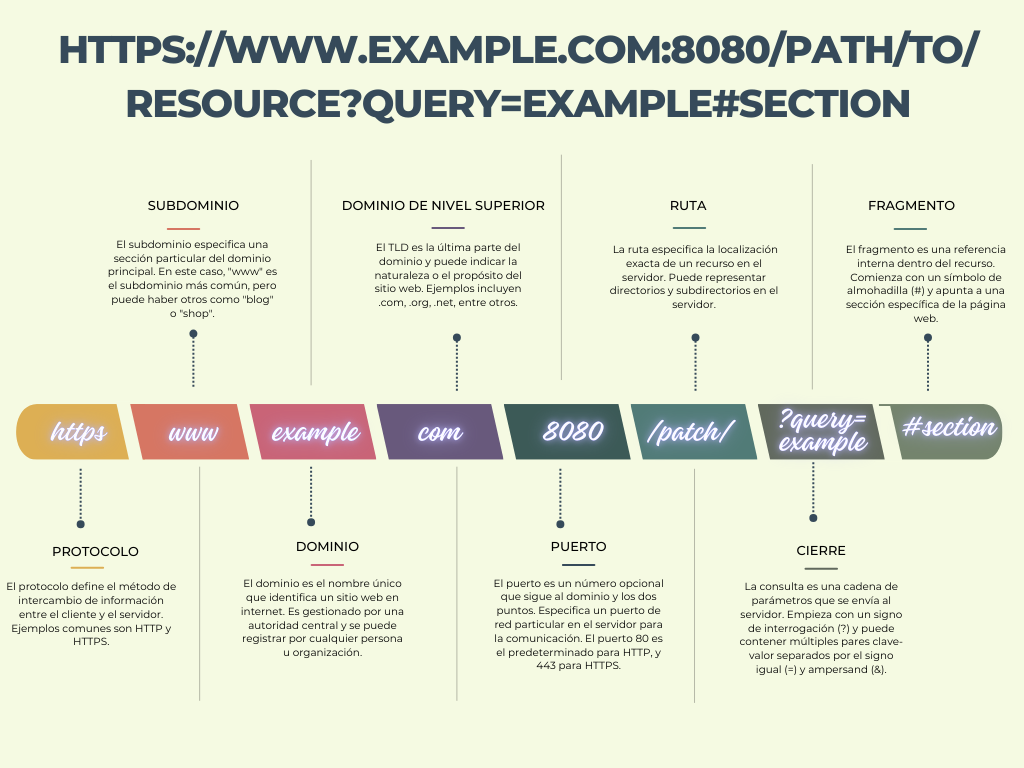
\includegraphics[width=0.8\textwidth]{urlPartes.png}
    \caption{Partes de una URL}
    \label{fig:partes_url}
\end{figure}

\begin{itemize}
    \item \textbf{Protocolo}: Define el método de intercambio de información entre el cliente y el servidor. Ejemplos comunes son HTTP y HTTPS.
    \item \textbf{Subdominio}: Especifica una sección particular del dominio principal.
    \item \textbf{Dominio}: Es el nombre único que identifica un sitio web en internet.
    \item \textbf{TLD (\gls{tld})}: Es el último segmento de un nombre de dominio.
    \item \textbf{Puerto}: Un número opcional que identifica una comunicación específica en el servidor.
    \item \textbf{Ruta}: Especifica la localización exacta de un recurso en el servidor.
    \item \textbf{Cierre}: Una cadena de parámetros que se envía al servidor.
    \item \textbf{Fragmento}: Una referencia interna dentro del recurso.
\end{itemize}

Una \textit{URL maliciosa} es una dirección web diseñada con la intención de engañar o perjudicar a los usuarios. Estas URLs son utilizadas por ciberdelincuentes para llevar a cabo ataques como \textit{\gls{phishing}}, distribución de malware, o redirección a sitios web fraudulentos. Las URLs maliciosas pueden parecer legítimas, imitando sitios web conocidos, o pueden tener componentes sospechosos como:

\begin{itemize}
    \item \textbf{Subdominios inusuales}: Para parecer confiables, algunas URLs maliciosas utilizan subdominios que imitan los legítimos.
    \item \textbf{TLDs no comunes}: Utilizan TLDs poco frecuentes para evadir filtros de seguridad.
    \item \textbf{Rutas y parámetros complejos}: Pueden incluir rutas o parámetros que parecen legítimos pero que redirigen a contenido malicioso.
    \item \textbf{Caracteres codificados}: Utilizan caracteres especiales o codificaciones que ocultan la verdadera intención de la URL.
\end{itemize}

La detección de URLs maliciosas es un desafío constante debido a la rapidez con la que estas pueden ser modificadas y la diversidad de técnicas utilizadas por los atacantes para evitar la detección. Nuestro estudio se enfoca en desarrollar métodos avanzados para identificar y mitigar estas amenazas a través de técnicas de \textit{machine learning} y análisis de características detalladas de las URLs.

                                                      
\subsection{Técnicas de Detección de URLs Maliciosas}
En esta subsección se describen las diferentes técnicas utilizadas para la detección de \glspl{url} maliciosas.

\subsubsection*{Análisis basado en listas negras}
El análisis basado en listas negras es uno de los métodos más comunes y efectivos para prevenir que los usuarios accedan a sitios web maliciosos. Este método implica el uso de una base de datos de \glspl{url} previamente identificadas como maliciosas. Cuando un usuario intenta acceder a una URL, esta se compara con la lista negra y, si hay una coincidencia, se bloquea el acceso.

Sun et al. propusieron un enfoque automatizado para la generación de listas negras de \glspl{url} utilizando una búsqueda por similitud\autocite{sun2016automating}. Otro enfoque de alto rendimiento para la búsqueda de \glspl{url} en sistemas de filtrado fue descrito por IEEE, destacando la eficiencia y utilización de memoria\autocite{ieee2010lookup}. Además, el sistema PhishNet utiliza técnicas predictivas para identificar nuevas \glspl{url} de phishing basadas en combinaciones simples de \glspl{url} conocidas\autocite{ieee2010phishnet}.

\subsubsection*{Análisis heurístico}
El análisis heurístico se basa en la utilización de reglas heurísticas para identificar \glspl{url} maliciosas. Estas reglas se derivan del análisis de características comunes en \glspl{url} maliciosas, como la longitud de la \gls{url}, la presencia de ciertos caracteres y patrones en el dominio.

Raja et al. propusieron un método para la detección de \glspl{url} maliciosas utilizando un enfoque basado en reglas heurísticas, destacando su efectividad en la generalización de \glspl{url} maliciosas\autocite{raja2022mudhr}. Por otro lado, Begum y Badugu realizaron un estudio comparativo de técnicas de detección de \glspl{url} maliciosas utilizando enfoques heurísticos y de aprendizaje automático\autocite{begum2019study}.

\subsubsection*{Análisis de contenido}
El análisis de contenido implica la inspección del contenido real de una página web para determinar si es maliciosa. Esto puede incluir el análisis de palabras clave, la inspección de scripts y el análisis del comportamiento de la página.

Un estudio sobre la detección de contenido web malicioso utilizando técnicas de aprendizaje automático fue presentado por IEEE, donde se desarrolló una extensión para Chrome para actuar como intermediario entre los usuarios y los sitios web maliciosos\autocite{ieee2017malicious}. Además, Xu et al. propusieron un enfoque de detección de sitios web maliciosos que analiza simultáneamente el tráfico de red y el contenido de la página web\autocite{xu2013cross}.

\subsubsection*{Métodos de machine learning}
Los métodos de aprendizaje automático han ganado popularidad en la detección de \glspl{url} maliciosas debido a su capacidad para aprender y adaptarse a nuevas amenazas. Estos métodos implican el uso de algoritmos de clasificación para identificar \glspl{url} maliciosas basándose en características extraídas de las \glspl{url}.






\subsection{Herramientas y Soluciones Existentes}
En esta subsección se realiza un análisis de las herramientas y soluciones actualmente disponibles en el mercado para la detección de \glspl{url} maliciosas. Se destacan sus características principales y se discuten sus limitaciones.

\subsubsection*{VirusTotal}
VirusTotal es un servicio gratuito que analiza archivos y \glspl{url} sospechosas, facilitando la detección rápida de virus, gusanos, troyanos y otros tipos de contenido malicioso. VirusTotal utiliza múltiples motores antivirus y herramientas de detección de malware para proporcionar resultados completos y detallados\autocite{peng2019opening}.

Una de las principales ventajas de VirusTotal es su capacidad para agregar resultados de múltiples motores de detección, lo que aumenta la probabilidad de identificar contenido malicioso. Sin embargo, también presenta limitaciones, como la posibilidad de falsos positivos y la falta de análisis en tiempo real para algunas amenazas emergentes\autocite{ieee2017automated}. Además, la variabilidad en los resultados entre diferentes motores de detección puede generar inconsistencias, lo que resalta la necesidad de metodologías más rigurosas para evaluar y utilizar los resultados obtenidos de VirusTotal\autocite{misquitta2024comparative}.

\subsubsection*{OpenPhish}
OpenPhish es un proveedor de servicios de inteligencia de amenazas que se especializa en la detección de \glspl{url} de phishing. Utiliza técnicas avanzadas de detección automatizada para identificar \glspl{url} maliciosas y proporciona una base de datos actualizada que puede integrarse con diversas soluciones de seguridad\cite{ieee2021comparative}.

OpenPhish destaca por su enfoque en la automatización y la actualización constante de su base de datos de \glspl{url} de phishing. Sin embargo, su eficacia puede verse limitada por la rapidez con la que se identifican y añaden nuevas \glspl{url} a la base de datos, así como por su enfoque específico en el phishing, dejando de lado otras formas de contenido malicioso.

\subsubsection*{DNS-Based Blackhole List (DNSBL)}
Las listas negras basadas en DNS (DNSBL) son un método para identificar y bloquear \glspl{url} maliciosas a nivel de sistema de nombres de dominio (DNS). Estas listas negras se utilizan comúnmente para filtrar correo electrónico no deseado y bloquear el acceso a sitios web maliciosos\autocite{fejrskov2021using}.

Las DNSBL son eficaces para bloquear una gran cantidad de \glspl{url} maliciosas conocidas. Sin embargo, presentan limitaciones, como la posibilidad de falsos positivos y la dependencia de actualizaciones constantes para mantener su efectividad contra nuevas amenazas. Además, el uso de DNSBL puede no ser suficiente para bloquear todo el tráfico malicioso, especialmente si los atacantes utilizan técnicas de evasión avanzadas.

\subsubsection*{Automated Threat Intelligence and Detection}
El uso de inteligencia artificial y aprendizaje automático en la detección automatizada de amenazas ha aumentado en los últimos años. Estas tecnologías pueden analizar grandes volúmenes de datos y detectar patrones de comportamiento malicioso, mejorando la capacidad de las organizaciones para identificar y responder a amenazas en tiempo real\autocite{ieee2020threat}.

La principal ventaja de la detección automatizada de amenazas es su capacidad para adaptarse y aprender de nuevas amenazas. Sin embargo, su eficacia depende de la calidad de los datos de entrenamiento y de los algoritmos utilizados, así como de la capacidad de la organización para implementar y gestionar estas tecnologías de manera efectiva. Un enfoque de clustering no supervisado, como el k-means, puede proporcionar valiosos conocimientos sobre las \glspl{url} maliciosas y ayudar a los operadores de red a tomar decisiones de política para mitigar los ciberataques\autocite{ieee2020threat}.

\subsubsection*{Comparativa de Herramientas de Detección de URLs Maliciosas}
La comparativa de herramientas de detección de \glspl{url} maliciosas revela que cada solución tiene sus propias fortalezas y debilidades. VirusTotal y OpenPhish son eficaces para identificar una amplia gama de amenazas, mientras que las listas negras basadas en DNS proporcionan un filtrado eficaz a nivel de red. La detección automatizada de amenazas ofrece una solución adaptable y escalable para organizaciones con grandes volúmenes de datos.

Sin embargo, todas estas herramientas comparten una limitación común: la necesidad de actualizaciones constantes y la posibilidad de falsos positivos y negativos. La integración de múltiples herramientas y enfoques puede mejorar la capacidad de detección general, pero también puede aumentar la complejidad y los costos de gestión.

\subsection{Limitaciones}

El sistema de detección de URLs maliciosas desarrollado presenta varias limitaciones que deben tenerse en cuenta:

\begin{itemize}
    \item \textbf{Dependencia de la Disponibilidad de la URL:} El \textit{extractor}, que es una clase en \textit{Python}, depende de que la URL esté en línea para extraer ciertas características, como la presencia de scripts o caracteres no decodificables. Si el servidor donde está alojada la URL está muy lejos, el tiempo de extracción de características puede aumentar significativamente.
    
    \item \textbf{Rapidez del Cambio de las URLs:} Las URLs maliciosas cambian rápidamente. Los atacantes crean clones muy buenos de sitios legítimos que son difíciles de detectar. Además, las URLs maliciosas activas son difíciles de encontrar porque suelen ser eliminadas rápidamente por las autoridades o los atacantes las mantienen en línea solo por un corto periodo para evitar ser rastreadas.

    \item \textbf{Contenido Dinámico y Malicioso:} Hay sitios web que inicialmente son benignos (como \textit{GitHub}), pero que pueden alojar contenido malicioso que los usuarios pueden descargar. Asimismo, sitios como \textit{Mil Anuncios} pueden tener anuncios que son fraudulentos, aunque el sitio en sí no lo sea.

    \item \textbf{Limitaciones del Modelo:} Los modelos de \textit{machine learning} utilizados son buenos para detectar URLs maliciosas basándose en sus características, pero no analizan el contenido dentro de la página ni las acciones de los scripts presentes. Esto significa que el sistema puede no detectar actividades maliciosas que ocurren una vez que se carga la página.

    \item \textbf{Disponibilidad de Datos Maliciosos:} Es difícil obtener un conjunto de datos suficientemente amplio y representativo de URLs maliciosas activas. Muchas de estas URLs son eliminadas rápidamente, lo que dificulta su recopilación y análisis en tiempo real.
\end{itemize}
                                     %$$
                                                                         %$$
                              %$$
                                                                         %$$
%************************************************************************%$$
%                                                                        %$$
%                      FIN de Estado del arte                            %$$
%                                                                        %$$
%========================================================================%$$

\newpage

%========================================================================%$$
%                                                                        %$$
%                                Bacula                                  %$$
%                                                                        %$$
%========================================================================%$$
                                                                         %$$
\section{Metodología}                                                         %$$
\subsection{Enfoque}

\subsection{Enfoque}

Este proyecto se ha organizado en cuatro fases principales, cada una de las cuales está alineada con las asignaturas del máster en Ciencia de Datos y Big Data. A continuación se detallan las fases y las asignaturas involucradas en cada una:
\begin{figure}[H]
    \centering
    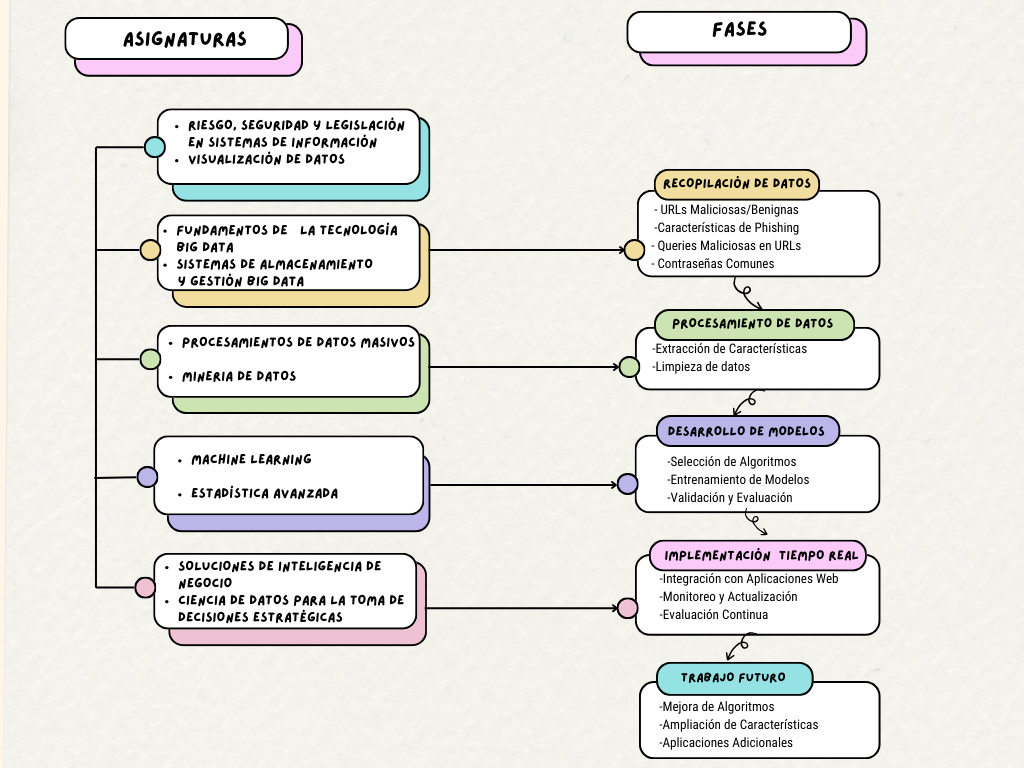
\includegraphics[width=0.8\textwidth]{imagenn1.png}
    \caption{Fases del Proyecto y Asignaturas del Máster}
\end{figure}
\begin{enumerate}
    \item \textbf{Recopilación de Datos}: 
    \begin{itemize}
        \item Asignaturas: Fundamentos de la Tecnología Big Data, Sistemas de Almacenamiento y Gestión Big Data.
        \item Actividades: Recolección de URLs maliciosas y benignas, características de phishing, queries maliciosas en URLs y contraseñas comunes.
    \end{itemize}

    \item \textbf{Procesamiento de Datos}:
    \begin{itemize}
        \item Asignaturas: Procesamientos de Datos Masivos, Minería de Datos.
        \item Actividades: Extracción de características y limpieza de datos.
    \end{itemize}

    \item \textbf{Desarrollo de Modelos}:
    \begin{itemize}
        \item Asignaturas: Machine Learning, Estadística Avanzada.
        \item Actividades: Selección de algoritmos, entrenamiento de modelos, validación y evaluación.
    \end{itemize}

    \item \textbf{Implementación en Tiempo Real}:
    \begin{itemize}
        \item Asignaturas: Soluciones de Inteligencia de Negocio, Ciencia de Datos para la Toma de Decisiones Estratégicas.
        \item Actividades: Integración con aplicaciones web, monitoreo y actualización, evaluación continua.
    \end{itemize}
\end{enumerate}

El sistema desarrollado consta de varios componentes clave, como se ilustra en las figuras a continuacion. A continuación se describe el flujo del sistema:
\begin{figure}[H]
    \centering
    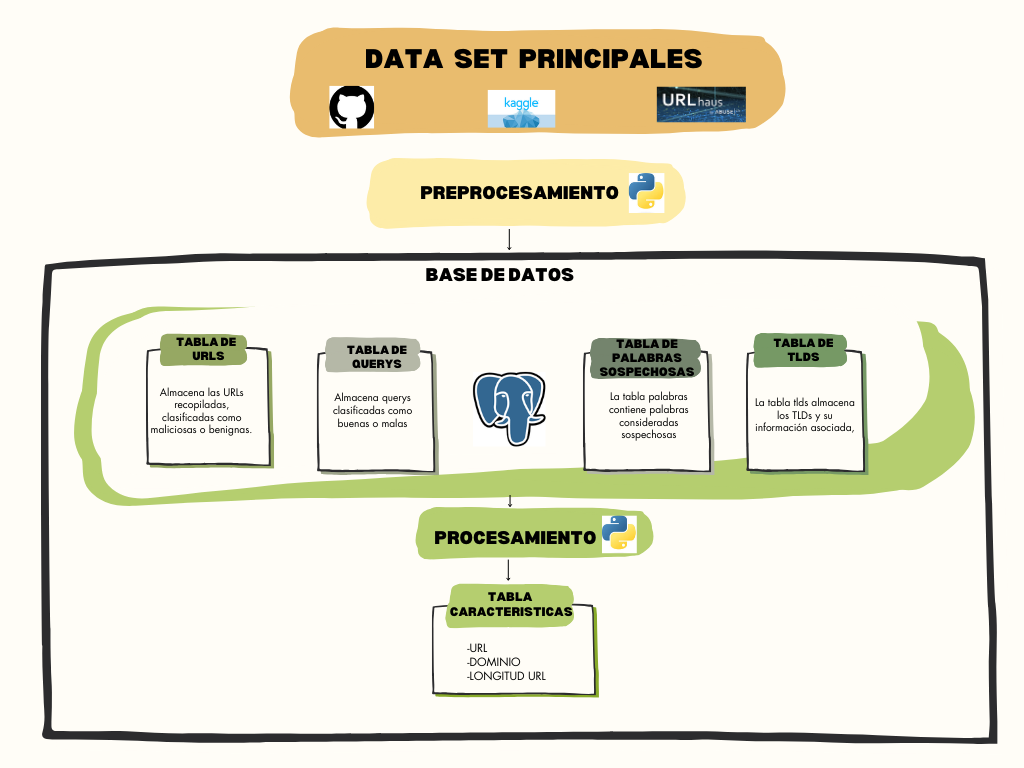
\includegraphics[width=0.8\textwidth]{imagenn2.png}
    \caption{Arquitectura del Sistema: Dataset, Preprocesamiento y Base de Datos}
\end{figure}

\begin{figure}[H]
    \centering
    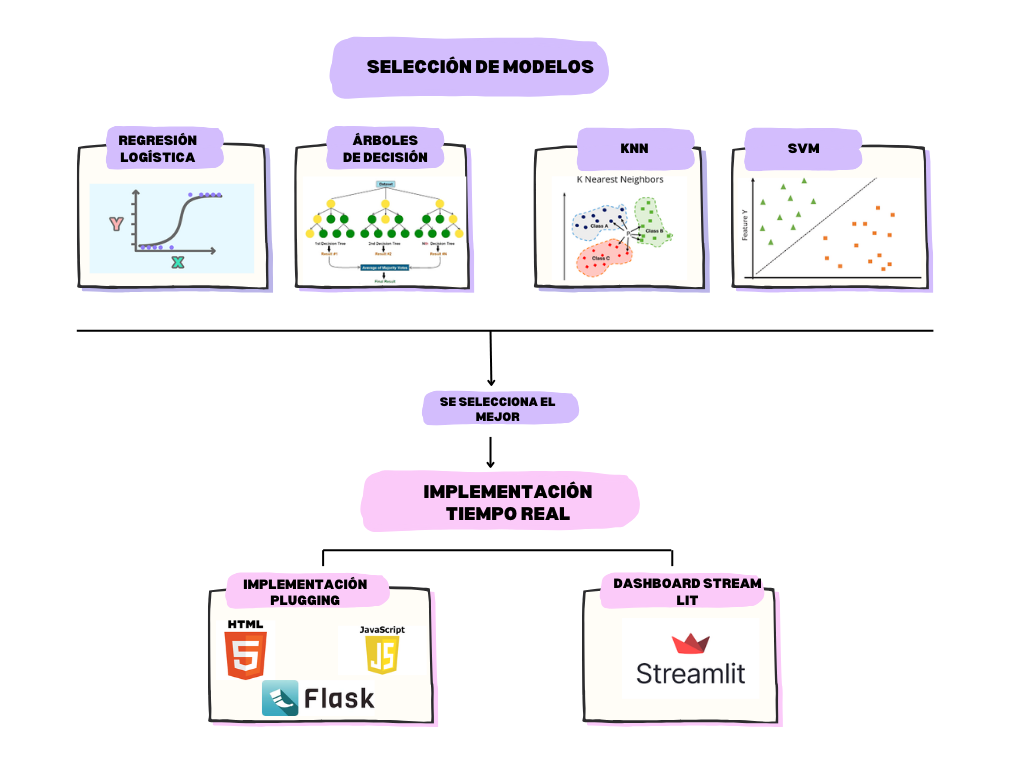
\includegraphics[width=0.8\textwidth]{imagenn3.png}
    \caption{Selección de Modelos e Implementación en Tiempo Real}
\end{figure}

\begin{itemize}
    \item \textbf{Dataset Principal y Preprocesamiento}: 
    Los datos recopilados de fuentes como Kaggle, GitHub y URLhaus son preprocesados usando Python y almacenados en una base de datos estructurada (Figura 2).
    
    \item \textbf{Base de Datos y Tablas de Características}: 
    La base de datos contiene tablas para almacenar URLs, queries, palabras sospechosas y TLDs. Las características extraídas de las URLs se almacenan en una tabla específica de características (Figura 2).
    
    \item \textbf{Selección y Entrenamiento de Modelos}: 
    Se evaluaron varios algoritmos de machine learning, incluyendo regresión logística, árboles de decisión, KNN y SVM, para seleccionar el mejor modelo para la detección de URLs maliciosas (Figura 3).
    
    \item \textbf{Implementación en Tiempo Real}: 
    El modelo seleccionado se implementó en un plugin usando HTML, JavaScript y Flask, y se desarrolló un dashboard interactivo con Streamlit para la visualización y análisis de datos (Figura 3).
\end{itemize}

Las herramientas utilizadas en este proyecto incluyen Python para el procesamiento de datos y desarrollo de modelos, Google Documents y GitHub para la documentación y gestión de versiones, Trello para la gestión del proyecto, Visual Studio para el desarrollo de código, Overleaf para la escritura de LaTeX, PowerPoint para las presentaciones, y Streamlit para el desarrollo del dashboard.




\subsection{Recopilación de Datos}

Los datos necesarios para este trabajo se han extraído utilizando \glspl{script} en Python y se han almacenado en una base de datos PostgreSQL. Los \glspl{script} que muestran cómo se obtienen estos datos están disponibles en mi repositorio de GitHub: \url{https://github.com/Fernando-Ares-Robledo/URL-detection}.

Esta base de datos PostgreSQL contiene varias tablas que se han poblado con diferentes fuentes de datos:

\subsubsection*{Tabla de URLs}
La tabla \texttt{urls} almacena las \glspl{url} recopiladas, clasificadas como maliciosas o benignas. Los datos para esta tabla provienen de las siguientes fuentes:
\begin{itemize}
    \item URLhaus - Malware URL exchange (\url{https://urlhaus.abuse.ch/}).
    \item Radek Hranický, et al. (2023). \textit{Phishing and Benign Domain Dataset (DNS, IP, WHOIS/RDAP, TLS, GeoIP)} (\url{https://doi.org/10.5281/zenodo.8364668}).
    \item 15 million Domain Names Dataset (\url{https://www.kaggle.com/datasets/aayushah19/dga-or-benign-domain-names?resource=download}).
\end{itemize}

La estructura de esta tabla es la siguiente:
\begin{itemize}
    \item \texttt{url} (text, no nulo): Almacena la \gls{url} completa.
    \item \texttt{maligna} (boolean, no nulo): Indica si la \gls{url} es maliciosa (true) o benigna (false).
    \item \texttt{tipo} (text, no nulo): Especifica el tipo de \gls{url}, por ejemplo, \texttt{phishing} o \texttt{benigna}.
\end{itemize}

\subsubsection*{Tabla de Queries}
La tabla \texttt{queries} almacena \glspl{query} clasificadas como buenas o malas, con datos provenientes de:
\begin{itemize}
    \item Faizann. \textit{GitHub - faizann24/Fwaf-Machine-Learning-driven-Web-Application-Firewall} (\url{https://github.com/faizann24/Fwaf-Machine-Learning-driven-Web-Application-Firewall}).
\end{itemize}

La estructura de esta tabla es la siguiente:
\begin{itemize}
    \item \texttt{id} (integer, no nulo, clave primaria, autoincremental): Identificador único para cada \gls{query}.
    \item \texttt{query} (text, no nulo): Almacena la \gls{query}.
    \item \texttt{buena} (boolean, no nulo): Indica si la \gls{query} es buena (true) o mala (false).
\end{itemize}

\subsubsection*{Tabla de Palabras Sospechosas}
La tabla \texttt{palabras} contiene palabras consideradas sospechosas, obtenidas de las siguientes fuentes:
\begin{itemize}
    \item Danielmiessler. \textit{SecLists/Discovery/Web-Content/raft-large-words.txt} (\url{https://github.com/danielmiessler/SecLists/blob/master/Discovery/Web-Content/raft-large-words.txt}).
    \item Danielmiessler. \textit{SecLists/Passwords/Common-Credentials/10k-most-common.txt} (\url{https://github.com/danielmiessler/SecLists/blob/master/Passwords/Common-Credentials/10k-most-common.txt}).
\end{itemize}

La estructura de esta tabla es la siguiente:
\begin{itemize}
    \item \texttt{id} (integer, no nulo, clave primaria, autoincremental): Identificador único para cada palabra.
    \item \texttt{palabra} (text, no nulo): Almacena la palabra sospechosa.
    \item \texttt{tipo} (text, no nulo): Especifica el tipo de palabra, por ejemplo, \texttt{común} o \texttt{contenido web}.
\end{itemize}

\subsubsection*{Tabla de TLDs}
La tabla \texttt{tlds} almacena los \glspl{tld} y su información asociada, con datos obtenidos de:
\begin{itemize}
    \item Root Zone Database (\url{https://www.iana.org/domains/root/db}).
\end{itemize}

La estructura de esta tabla es la siguiente:
\begin{itemize}
    \item \texttt{id} (integer, no nulo, clave primaria, autoincremental): Identificador único para cada \gls{tld}.
    \item \texttt{domain} (text, no nulo): Almacena el \gls{tld}, por ejemplo, \texttt{.com} o \texttt{.org}.
    \item \texttt{type} (text, opcional): Especifica el tipo de \gls{tld}, como \texttt{genérico} o \texttt{código de país}.
    \item \texttt{tld\_manager} (text, opcional): Indica la organización responsable de la gestión del \gls{tld}.
\end{itemize}

Estas tablas serán utilizadas para crear una nueva tabla con las características de las \glspl{url}, la cual se definirá en la siguiente sección.

\subsection{Extracción de Características}

La extracción de características de las \glspl{url} se realiza mediante un \gls{script} en Python, el cual está disponible en el repositorio de GitHub (\url{https://github.com/Fernando-Ares-Robledo/URL-detection}). Este \gls{script} se encarga de procesar cada \gls{url} y almacenar las características extraídas en una tabla llamada \texttt{CaracteristicasURLs} en la base de datos PostgreSQL. A continuación, se describen las principales funcionalidades del \gls{script} y las características extraídas.

\subsubsection*{Descripción del Script}

El \gls{script} realiza las siguientes acciones:

\begin{enumerate}
    \item Conexión a la base de datos PostgreSQL y creación de la tabla \texttt{CaracteristicasURLs} si no existe.
    \item Procesamiento de cada \gls{url}, asegurando que comiencen con \texttt{http://} o \texttt{https://}.
    \item Extracción de características relacionadas con la longitud de la \gls{url}, la cantidad de ciertos caracteres, y otras propiedades léxicas.
    \item Resolución del dominio a una dirección IP y obtención de su ubicación geográfica.
    \item Verificación de la presencia de palabras sospechosas, cadenas hexadecimales y redirecciones.
    \item Extracción de información de \gls{whois} y verificación del estado del dominio.
    \item Verificación de si la \gls{url} está indexada en Google y si contiene scripts o caracteres no decodificables.
    \item Inserción de las características extraídas en la tabla \texttt{CaracteristicasURLs}.
\end{enumerate}

\subsubsection*{Características Extraídas}

A continuación, se describen las características extraídas por el \gls{script}:

\begin{itemize}
    \item \texttt{url} (text): La \gls{url} completa.
    \item \texttt{longitud} (integer): Longitud de la \gls{url}.
    \item \texttt{cantidad\_digitos} (integer): Cantidad de dígitos en la \gls{url}.
    \item \texttt{cantidad\_letras} (integer): Cantidad de letras en la \gls{url}.
    \item \texttt{count\_punto} (integer): Cantidad de puntos (\texttt{.}) en la \gls{url}.
    \item \texttt{count\_guion} (integer): Cantidad de guiones (\texttt{-}) en la \gls{url}.
    \item \texttt{count\_guion\_bajo} (integer): Cantidad de guiones bajos (\texttt{\_}) en la \gls{url}.
    \item \texttt{count\_slash} (integer): Cantidad de barras (\texttt{/}) en la \gls{url}.
    \item \texttt{count\_interrogacion} (integer): Cantidad de signos de interrogación (\texttt{?}) en la \gls{url}.
    \item \texttt{count\_igual} (integer): Cantidad de signos de igual (\texttt{=}) en la \gls{url}.
    \item \texttt{count\_arroba} (integer): Cantidad de arrobas (\texttt{@}) en la \gls{url}.
    \item \texttt{count\_ampersand} (integer): Cantidad de ampersands (\texttt{\&}) en la \gls{url}.
    \item \texttt{count\_exclamacion} (integer): Cantidad de signos de exclamación (\texttt{!}) en la \gls{url}.
    \item \texttt{count\_espacio} (integer): Cantidad de espacios (\texttt{ }) en la \gls{url}.
    \item \texttt{count\_tilde} (integer): Cantidad de tildes (\texttt{\textasciitilde}) en la \gls{url}.
    \item \texttt{count\_coma} (integer): Cantidad de comas (\texttt{,}) en la \gls{url}.
    \item \texttt{count\_mas} (integer): Cantidad de signos de más (\texttt{+}) en la \gls{url}.
    \item \texttt{count\_asterisco} (integer): Cantidad de asteriscos (\texttt{*}) en la \gls{url}.
    \item \texttt{count\_numeral} (integer): Cantidad de numerales (\texttt{\#}) en la \gls{url}.
    \item \texttt{count\_dolar} (integer): Cantidad de signos de dólar (\texttt{\$}) en la \gls{url}.
    \item \texttt{count\_porcentaje} (integer): Cantidad de signos de porcentaje (\texttt{\%}) en la \gls{url}.
    \item \texttt{domain} (text): Dominio de la \gls{url}.
    \item \texttt{domain\_length} (integer): Longitud del dominio.
    \item \texttt{cantidad\_vocales\_dominio} (integer): Cantidad de vocales en el dominio.
    \item \texttt{dominio\_resuelve\_a\_ip} (boolean): Indica si el dominio se resuelve a una dirección IP.
    \item \texttt{directory} (text): Directorio de la \gls{url}.
    \item \texttt{directory\_length} (integer): Longitud del directorio.
    \item \texttt{file} (text): Archivo de la \gls{url}.
    \item \texttt{file\_length} (integer): Longitud del archivo.
    \item \texttt{parameters} (text): Parámetros de la \gls{url}.
    \item \texttt{parameters\_length} (integer): Longitud de los parámetros.
    \item \texttt{tld} (text): \gls{tld} del dominio.
    \item \texttt{tld\_present} (boolean): Indica si el \gls{tld} está presente en la base de datos.
    \item \texttt{numero\_parametros} (integer): Número de parámetros en la \gls{url}.
    \item \texttt{email\_presente} (boolean): Indica si hay un correo electrónico en la \gls{url}.
    \item \texttt{tls\_version} (text): Versión de \gls{tls} utilizada.
    \item \texttt{tld\_type} (text): Tipo de \gls{tld}.
    \item \texttt{tld\_manager} (text): Administrador del \gls{tld}.
    \item \texttt{whois\_registrar} (text): Registrador de \gls{whois}.
    \item \texttt{whois\_creation\_date} (timestamp): Fecha de creación de \gls{whois}.
    \item \texttt{whois\_expiration\_date} (timestamp): Fecha de expiración de \gls{whois}.
    \item \texttt{whois\_updated\_date} (timestamp): Fecha de actualización de \gls{whois}.
    \item \texttt{whois\_status} (text): Estado de \gls{whois}.
    \item \texttt{es\_acortada} (boolean): Indica si la \gls{url} está acortada.
    \item \texttt{numero\_subdominios} (integer): Número de subdominios.
    \item \texttt{entropia\_sld} (float): Entropía del \gls{sld}.
    \item \texttt{ciudad} (text): Ciudad de la IP.
    \item \texttt{pais} (text): País de la IP.
    \item \texttt{lon}(float): longitud.
    \item \texttt{lat}(float): latitud.
    \item \texttt{dominio\_benigno} (integer): Indica si el dominio es benigno (1), malicioso (-1) o desconocido (0).
    \item \texttt{tiene\_palabras\_sospechosas} (boolean): Indica si contiene palabras sospechosas.
    \item \texttt{palabras\_detectadas} (text): Palabras sospechosas detectadas.
    \item \texttt{tiene\_hexadecimal} (boolean): Indica si contiene cadenas hexadecimales.
    \item \texttt{redirige} (boolean): Indica si la \gls{url} redirige.
    \item \texttt{esta\_registrada} (boolean): Indica si el dominio está registrado.
    \item \texttt{esta\_online} (boolean): Indica si la \gls{url} está en línea.
    \item \texttt{tiene\_directorios} (boolean): Indica si contiene directorios.
    \item \texttt{tiene\_file} (boolean): Indica si contiene un archivo.
    \item \texttt{edad\_dominio} (integer): Edad del dominio en días.
    \item \texttt{tiempo\_restante} (integer): Tiempo restante hasta la expiración del dominio en días.
    \item \texttt{queries\_buenas} (boolean): Indica si contiene \glspl{query} buenas.
    \item \texttt{queries\_malas} (boolean): Indica si contiene \glspl{query} malas.
    \item \texttt{maligna} (boolean): Indica si la \gls{url} es maliciosa.
    \item \texttt{tiene\_puerto} (boolean): Indica si contiene un puerto.
    \item \texttt{dominio\_es\_ip} (boolean): Indica si el dominio es una IP.
    \item \texttt{usa\_https} (boolean): Indica si usa HTTPS.
    \item \texttt{indexada\_en\_google} (boolean): Indica si está indexada en Google.
    \item \texttt{tiene\_tls} (boolean): Indica si tiene \gls{tls}.
    \item \texttt{dominio\_registrado} (boolean): Indica si el dominio está registrado.
    \item \texttt{contiene\_scripts} (boolean): Indica si contiene scripts.
    \item \texttt{contiene\_caracteres\_no\_decodificables} (boolean): Indica si contiene caracteres no decodificables.
    \item \texttt{tiene\_iframe}(bolean): Indica si contiene un iframe en la web.
    \item \texttt{tiempo\_respuesta}(float): Indica el tiempo respuesta entre servidor y cliente.
    \item \texttt{tiene\_redes\_sociales}(bolean): Indica tiene alguna red social.
\end{itemize}

La tabla \texttt{CaracteristicasURLs} almacena todas estas características para cada \gls{url} procesada. Estas características serán utilizadas en las siguientes fases del proyecto para el entrenamiento y evaluación de modelos de \textit{machine learning}.

\subsection{Desarrollo del Modelo}

\subsubsection*{Descripción de los algoritmos de \textit{Machine Learning} utilizados}
En este proyecto, se emplearon múltiples algoritmos de \textit{machine learning} para la detección de \glspl{url} maliciosas. Los algoritmos utilizados fueron:

\begin{itemize}
    \item \textbf{Árbol de Decisión}: 
    \begin{itemize}
        \item Búsqueda Aleatoria de Hiperparámetros (Random Search)
        \item Búsqueda Exhaustiva de Hiperparámetros (Grid Search)
    \end{itemize}
    \item \textbf{Bosque Aleatorio (\textit{Random Forest})}: 
    \begin{itemize}
        \item Búsqueda Aleatoria de Hiperparámetros (Random Search)
        \item Búsqueda Exhaustiva de Hiperparámetros (Grid Search)
    \end{itemize}
    \item \textbf{K-Vecinos más Cercanos (\textit{K-Nearest Neighbors, KNN})}: 
    \begin{itemize}
        \item Búsqueda Aleatoria de Hiperparámetros (Random Search)
        \item Búsqueda Exhaustiva de Hiperparámetros (Grid Search)
    \end{itemize}
    \item \textbf{XGBoost}: 
    \begin{itemize}
        \item Búsqueda Aleatoria de Hiperparámetros (Random Search)
        \item Búsqueda Exhaustiva de Hiperparámetros (Grid Search)
    \end{itemize}
    \item \textbf{Máquina de Soporte Vectorial (\textit{Support Vector Machine, SVM})}
    \item \textbf{LightGBM (\textit{Light Gradient Boosting Machine})}: 
    \begin{itemize}
        \item Búsqueda Aleatoria de Hiperparámetros (Random Search)
        \item Búsqueda Exhaustiva de Hiperparámetros (Grid Search)
    \end{itemize}
    \item \textbf{Gradient Boosting}: 
    \begin{itemize}
        \item Búsqueda Aleatoria de Hiperparámetros (Random Search)
        \item Búsqueda Exhaustiva de Hiperparámetros (Grid Search)
    \end{itemize}
    \item \textbf{AdaBoost}: 
    \begin{itemize}
        \item Búsqueda Aleatoria de Hiperparámetros (Random Search)
        \item Búsqueda Exhaustiva de Hiperparámetros (Grid Search)
    \end{itemize}
    \item \textbf{Regresión Logística}: 
    \begin{itemize}
        \item Búsqueda Aleatoria de Hiperparámetros (Random Search)
    \end{itemize}
\end{itemize}



\subsubsection{Modelos de Stacking Utilizados}

En el proyecto se implementaron dos modelos de \textit{stacking} para mejorar la precisión y robustez de la detección de \glspl{url} maliciosas. 

\textbf{Primer Modelo de Stacking}
El primer modelo de \textit{stacking} combina las predicciones de todos los modelos base mencionados anteriormente. Este enfoque permite aprovechar las fortalezas de diferentes algoritmos y minimizar sus debilidades individuales. Se utilizó un meta-modelo de \textit{Logistic Regression} para combinar las predicciones de los modelos base y generar la predicción final.

\textbf{Segundo Modelo de Stacking}
El segundo modelo de \textit{stacking} aplica un enfoque más avanzado que considera diferentes subconjuntos de características y algoritmos para optimizar el rendimiento. Este modelo se construye de la siguiente manera:

\begin{enumerate}
    \item \textbf{Selección de Subconjuntos de Características}: Se crearon cuatro subconjuntos de características:
    \begin{itemize}
        \item \textbf{Conjunto 1}: Incluye las características \texttt{usa\_https}, \texttt{esta\_registrada}, \texttt{cantidad\_letras} y otras características restantes.
        \item \textbf{Conjunto 2}: Incluye todas las características excepto \texttt{usa\_https}.
        \item \textbf{Conjunto 3}: Incluye todas las características excepto \texttt{esta\_registrada}.
        \item \textbf{Conjunto 4}: Incluye todas las características excepto \texttt{cantidad\_letras}.
    \end{itemize}

    \item \textbf{Entrenamiento de Modelos Base}: Para cada subconjunto de características, se entrenaron los siguientes modelos:
    \begin{itemize}
        \item \textbf{Random Forest}
        \item \textbf{Logistic Regression}
        \item \textbf{XGBoost}
    \end{itemize}

    \item \textbf{Generación de Predicciones}: Las predicciones de cada modelo base se generaron para el conjunto de validación y prueba.

    \item \textbf{Entrenamiento del Meta-Modelo}: Un meta-modelo de \textit{Logistic Regression} se entrenó utilizando las predicciones generadas por los modelos base en el conjunto de validación. Este meta-modelo combina las predicciones para producir la predicción final.

    \item \textbf{Evaluación del Modelo}: El modelo de \textit{stacking} se evaluó utilizando las predicciones del conjunto de prueba para medir su precisión, falsos positivos y falsos negativos.
\end{enumerate}

El segundo modelo de \textit{stacking} es particularmente efectivo porque permite capturar interacciones complejas entre diferentes características y modelos base.




\subsubsection*{Detalles sobre el entrenamiento y la validación del modelo}
El proceso de entrenamiento y validación se llevó a cabo siguiendo estos pasos:

\begin{enumerate}
    \item \textbf{División del Conjunto de Datos}: 
    \begin{itemize}
        \item El conjunto de datos se dividió en tres subconjuntos: entrenamiento (60\%), validación (20\%) y prueba (20\%).
    \end{itemize}
    \item \textbf{Selección de Características}: 
    \begin{itemize}
        \item Se crearon diferentes subconjuntos de características para explorar cómo diferentes combinaciones afectan el rendimiento de los modelos.
    \end{itemize}
    \item \textbf{Entrenamiento de Modelos}: 
    \begin{itemize}
        \item Se entrenaron múltiples modelos utilizando diferentes algoritmos de \textit{machine learning} y se optimizaron los hiperparámetros utilizando búsquedas aleatorias y exhaustivas.
    \end{itemize}
    \item \textbf{Validación Cruzada}: 
    \begin{itemize}
        \item Se utilizó validación cruzada de 3 pliegues para asegurar que los modelos no estén sobreajustados y generalicen bien en datos no vistos.
    \end{itemize}
    \item \textbf{Evaluación del Meta-Modelo}: 
    \begin{itemize}
        \item Los meta-modelos de \textit{stacking} se entrenaron utilizando las predicciones de los modelos base en el conjunto de validación y se evaluaron tanto en el conjunto de validación como en el de prueba.
    \end{itemize}
\end{enumerate}

\subsubsection*{Métricas de evaluación empleadas}

Para evaluar el rendimiento de los modelos de \textit{machine learning} en la detección de \glspl{url} maliciosas, hemos seleccionado tres métricas clave: precisión, falsos positivos y falsos negativos. La elección de estas métricas se justifica por las siguientes razones:

\begin{itemize}
    \item \textbf{Precisión}: La precisión es una métrica fundamental en problemas de clasificación, especialmente en el contexto de la detección de \glspl{url} maliciosas. Se define como la proporción de verdaderos positivos (URLs maliciosas correctamente identificadas) entre el total de predicciones positivas (URLs predichas como maliciosas). La precisión es crucial porque queremos asegurarnos de que las URLs identificadas como maliciosas sean efectivamente maliciosas, minimizando las falsas alarmas.

    \item \textbf{Falsos Positivos (FP)}: Los falsos positivos ocurren cuando una URL benigna se clasifica incorrectamente como maliciosa. Esta métrica es esencial para evaluar porque un alto número de falsos positivos puede generar desconfianza en el sistema y causar interrupciones innecesarias. En un entorno real, un número elevado de falsos positivos podría resultar en la pérdida de acceso a recursos legítimos y generar alertas innecesarias, disminuyendo la usabilidad del sistema.

    \item \textbf{Falsos Negativos (FN)}: Los falsos negativos se producen cuando una URL maliciosa no es detectada y se clasifica erróneamente como benigna. Esta métrica es crítica porque un falso negativo implica que una amenaza potencial no ha sido identificada, lo que podría llevar a una brecha de seguridad. Minimizar los falsos negativos es vital para garantizar que el sistema de detección sea efectivo en la protección contra \gls{phishing} y otros ataques cibernéticos.

\end{itemize}

Aunque existen muchas otras métricas de evaluación en el campo del \textit{machine learning} (como \textit{recall}, \textit{F1 score}, área bajo la curva ROC, entre otras), la precisión, los falsos positivos y los falsos negativos han sido seleccionados debido a su relevancia directa en el contexto de la detección de \glspl{url} maliciosas. Estas métricas proporcionan una visión equilibrada del rendimiento del modelo, asegurando que las predicciones sean tanto precisas como fiables, mientras se minimizan los errores críticos que podrían comprometer la seguridad del sistema.
\subsection{Implementación en Tiempo Real}

Para la implementación en tiempo real del sistema de detección de \glspl{url} maliciosas, se ha desarrollado un \gls{plugin} para navegadores web utilizando \textit{JavaScript} y \textit{HTML}. Este \gls{plugin} se comunica con un servidor \textit{Flask} implementado en \textit{Python}, el cual aloja el modelo de \textit{machine learning} entrenado.

\subsubsection*{Arquitectura del Sistema}

La arquitectura del sistema se compone de los siguientes elementos:

\begin{itemize}
    \item \textbf{Plugin del Navegador}: Implementado en \textit{JavaScript} y \textit{HTML}, este \gls{plugin} intercepta las solicitudes de navegación del usuario. Cada vez que se accede a una nueva \gls{url}, el \gls{plugin} envía una solicitud al servidor \textit{Flask} para evaluar la \gls{url}.

    \item \textbf{Servidor \textit{Flask}}: Este servidor, implementado en \textit{Python}, recibe las solicitudes del \gls{plugin} del navegador y utiliza el mejor modelo de \textit{machine learning} para predecir si la \gls{url} es maligna o benigna. El servidor \textit{Flask} devuelve la predicción al \gls{plugin} del navegador en tiempo real.

    \item \textbf{Modelo de \textit{Machine Learning}}: El modelo entrenado y optimizado se aloja en el servidor \textit{Flask}. Este modelo ha sido seleccionado a partir de un exhaustivo proceso de evaluación y optimización, garantizando la máxima precisión y confiabilidad en la detección de \glspl{url} maliciosas.
\end{itemize}

\subsubsection*{Proceso de Detección en Tiempo Real}

El proceso de detección en tiempo real sigue los siguientes pasos:

\begin{enumerate}
    \item \textbf{Interceptación de la URL}: Cuando el usuario navega a una nueva \gls{url}, el \gls{plugin} del navegador intercepta la solicitud y captura la \gls{url} a ser visitada.

    \item \textbf{Envío de la Solicitud}: El \gls{plugin} envía la \gls{url} interceptada al servidor \textit{Flask} mediante una solicitud \textit{HTTP POST}.

    \item \textbf{Evaluación de la URL}: El servidor \textit{Flask} recibe la \gls{url} y utiliza el modelo de \textit{machine learning} para predecir si la \gls{url} es maligna o benigna.

    \item \textbf{Respuesta del Servidor}: El servidor \textit{Flask} devuelve la predicción al \gls{plugin} del navegador, indicando si la \gls{url} es segura o no.

    \item \textbf{Notificación al Usuario}: El \gls{plugin} del navegador muestra una notificación al usuario basada en la predicción del modelo. Si la \gls{url} es considerada maligna, el usuario recibe una advertencia y puede optar por no continuar a la página.
\end{enumerate}

\subsubsection*{Beneficios de la Implementación en Tiempo Real}

La implementación en tiempo real proporciona varios beneficios:

\begin{itemize}
    \item \textbf{Seguridad Inmediata}: Los usuarios reciben advertencias inmediatas sobre \glspl{url} potencialmente maliciosas, protegiéndolos de \gls{phishing} y otras amenazas en línea.

    \item \textbf{Experiencia de Usuario Mejorada}: Al integrar la detección directamente en el navegador, la experiencia del usuario es fluida y no intrusiva.

    \item \textbf{Actualización Dinámica}: El servidor \textit{Flask} permite actualizar y mejorar el modelo de \textit{machine learning} sin necesidad de modificar el \gls{plugin} del navegador, asegurando que el sistema se mantenga actualizado frente a nuevas amenazas.
\end{itemize}
\subsection{Implementación del \textit{Dashboard}}

Para la implementación del \gls{dashboard} se ha utilizado \textit{Streamlit}, una herramienta de código abierto que facilita la creación de aplicaciones web interactivas para el análisis de datos. Este \gls{dashboard} está diseñado para proporcionar dos funcionalidades principales: la evaluación en tiempo real de \glspl{url} introducidas por el usuario y el análisis de las características de las \glspl{url} almacenadas en la base de datos.

\subsubsection*{Funcionalidades del \textit{Dashboard}}

El \gls{dashboard} desarrollado en \textit{Streamlit} consta de dos partes principales:

\begin{itemize}
    \item \textbf{Evaluación en Tiempo Real de URLs}: Esta sección permite al usuario introducir una \gls{url} y obtener instantáneamente un análisis detallado de sus características y una predicción sobre si la \gls{url} es maligna o no. El proceso de evaluación incluye la extracción de características de la \gls{url} y la consulta al modelo de \textit{machine learning} alojado en el servidor \textit{Flask}.

    \item \textbf{Análisis de Características de URLs Almacenadas}: Esta sección del \gls{dashboard} proporciona una visualización interactiva de las características de las \glspl{url} almacenadas en la base de datos \textit{PostgreSQL}. Los usuarios pueden explorar diversas métricas y estadísticas clave, como la distribución geográfica de las \glspl{url}, la proporción de \glspl{url} benignas y malignas, y otros patrones relevantes.
\end{itemize}

\subsubsection*{Implementación del \textit{Dashboard} en \textit{Streamlit}}

La implementación del \gls{dashboard} en \textit{Streamlit} se realiza mediante un conjunto de scripts en \textit{Python} que integran diversas librerías de análisis de datos y visualización. A continuación, se describen los componentes clave del \gls{dashboard}:

\begin{itemize}
    \item \textbf{Interfaz de Usuario}: Utilizando \textit{Streamlit}, se ha diseñado una interfaz intuitiva y amigable que permite a los usuarios introducir \glspl{url} y visualizar los resultados del análisis. Los formularios y botones interactivos facilitan la navegación y el acceso a las diferentes funcionalidades del \gls{dashboard}.

    \item \textbf{Extracción de Características}: Al introducir una \gls{url}, el \gls{dashboard} realiza una solicitud al servidor \textit{Flask} para extraer las características de la \gls{url} y obtener una predicción sobre su naturaleza (benigna o maligna). Los resultados se presentan en un formato claro y comprensible para el usuario.

    \item \textbf{Visualización de Datos}: La sección de análisis de características utiliza librerías como \textit{Matplotlib} y \textit{Seaborn} para generar gráficos interactivos que muestran las estadísticas clave de las \glspl{url} almacenadas. Estas visualizaciones incluyen gráficos de barras, histogramas, mapas de calor y gráficos geográficos, proporcionando una comprensión profunda de los datos.

    \item \textbf{Conexión a la Base de Datos}: La integración con la base de datos \textit{PostgreSQL} permite al \gls{dashboard} acceder a las \glspl{url} almacenadas y sus características. Las consultas a la base de datos se realizan de manera eficiente para garantizar una experiencia de usuario fluida y rápida.
\end{itemize}

\subsubsection*{Beneficios del \textit{Dashboard}}

El \gls{dashboard} desarrollado proporciona varios beneficios significativos:

\begin{itemize}
    \item \textbf{Evaluación Instantánea}: Permite a los usuarios evaluar la seguridad de las \glspl{url} en tiempo real, proporcionando una herramienta valiosa para la protección contra \gls{phishing} y otras amenazas en línea.

    \item \textbf{Análisis Profundo}: Ofrece una visión detallada de las características y patrones de las \glspl{url} almacenadas, facilitando la identificación de tendencias y comportamientos sospechosos.

    \item \textbf{Interactividad y Usabilidad}: La interfaz intuitiva y las visualizaciones interactivas hacen que el \gls{dashboard} sea accesible y fácil de usar, incluso para usuarios sin experiencia técnica.
\end{itemize}

                                                                         %$$
%************************************************************************%$$
%                                                                        %$$
%                          FIN de Bacula                                 %$$
%                                                                        %$$
%========================================================================%$$







\newpage


\section{Resultados y Discusión}
\subsection{Resultados de la Extracción de Características}

En esta sección se presentan los resultados obtenidos de la extracción de características de las \glspl{url} analizadas. La extracción de características es un paso fundamental en el proceso de creación del modelo de detección de \gls{phishing} y otras amenazas web, ya que permite transformar las \glspl{url} en un conjunto de datos estructurados que pueden ser utilizados por los algoritmos de \textit{machine learning} para el entrenamiento y la predicción.

\subsubsection*{Estadísticas Descriptivas}

Las características extraídas y sus respectivas estadísticas descriptivas se resumen en los siguientes puntos:

\begin{itemize}
    \item \textbf{Longitud de la \gls{url}}: 
    La longitud de las \glspl{url} analizadas presenta una media que indica que la mayoría de las \glspl{url} son relativamente cortas, concentrándose entre 10 y 50 caracteres. Esto sugiere que las \glspl{url} en general tienden a ser más concisas.

    \item \textbf{Cantidad de Dígitos en la \gls{url}}: 
    La cantidad de dígitos en las \glspl{url} muestra una distribución sesgada hacia la izquierda, con la mayoría de las \glspl{url} conteniendo pocos dígitos. Esto puede estar relacionado con el intento de los atacantes de hacer las \glspl{url} más legítimas.

    \item \textbf{Cantidad de Letras en la \gls{url}}: 
    La distribución de la cantidad de letras en las \glspl{url} también está sesgada hacia la izquierda, indicando que la mayoría de las \glspl{url} contienen una cantidad moderada de letras, lo que puede ayudar a evitar la detección por parte de los usuarios.

    \item \textbf{Cantidad de Caracteres Especiales en la \gls{url}}: 
    Los caracteres especiales como puntos, guiones y guiones bajos son relativamente pocos en la mayoría de las \glspl{url}. Esto sugiere que las \glspl{url} maliciosas intentan mantener una apariencia simple para evitar la detección.

    \item \textbf{Longitud del Dominio}: 
    La longitud de los dominios en las \glspl{url} analizadas varía, pero la mayoría son relativamente cortos. Esto podría deberse a que los dominios más cortos son más fáciles de recordar y parecen más legítimos.

    \item \textbf{Cantidad de Vocales en el Dominio}: 
    La cantidad de vocales en el dominio varía considerablemente, lo que puede indicar que los atacantes utilizan una mezcla de nombres de dominio complejos y simples para evitar la detección.

    \item \textbf{Longitud del Directorio}: 
    La longitud del directorio en las \glspl{url} muestra una distribución sesgada hacia la izquierda, indicando que la mayoría de los directorios son cortos. Esto sugiere que las \glspl{url} maliciosas tienden a no profundizar en la estructura del sitio.

    \item \textbf{Número de Parámetros}: 
    La mayoría de las \glspl{url} tienen pocos parámetros, lo que sugiere que los atacantes prefieren mantener las \glspl{url} simples y fáciles de manejar.

    \item \textbf{Número de Subdominios}: 
    La cantidad de subdominios en las \glspl{url} es generalmente baja, lo que indica que los atacantes no suelen utilizar estructuras de dominio complejas.

    \item \textbf{Entropía del \gls{sld}}: 
    La entropía del \gls{sld} varía significativamente entre las \glspl{url}, lo que sugiere una diversidad en la complejidad de los nombres de los dominios utilizados en las \glspl{url} maliciosas.

    \item \textbf{Edad del Dominio (días)}: 
    La edad de los dominios varía ampliamente, con algunos dominios muy antiguos y otros muy recientes. Esto puede indicar que los atacantes utilizan tanto dominios nuevos como antiguos para sus ataques.

    \item \textbf{Tiempo Restante para la Expiración (días)}: 
    Similar a la edad del dominio, el tiempo restante para la expiración también varía ampliamente, lo que sugiere que los atacantes no tienen una preferencia clara en cuanto al tiempo de vida restante de un dominio.
\end{itemize}

\subsubsection*{Distribuciones de Características}

Las distribuciones de las características principales se representan en los siguientes histogramas:

\begin{figure}[H]
    \centering
    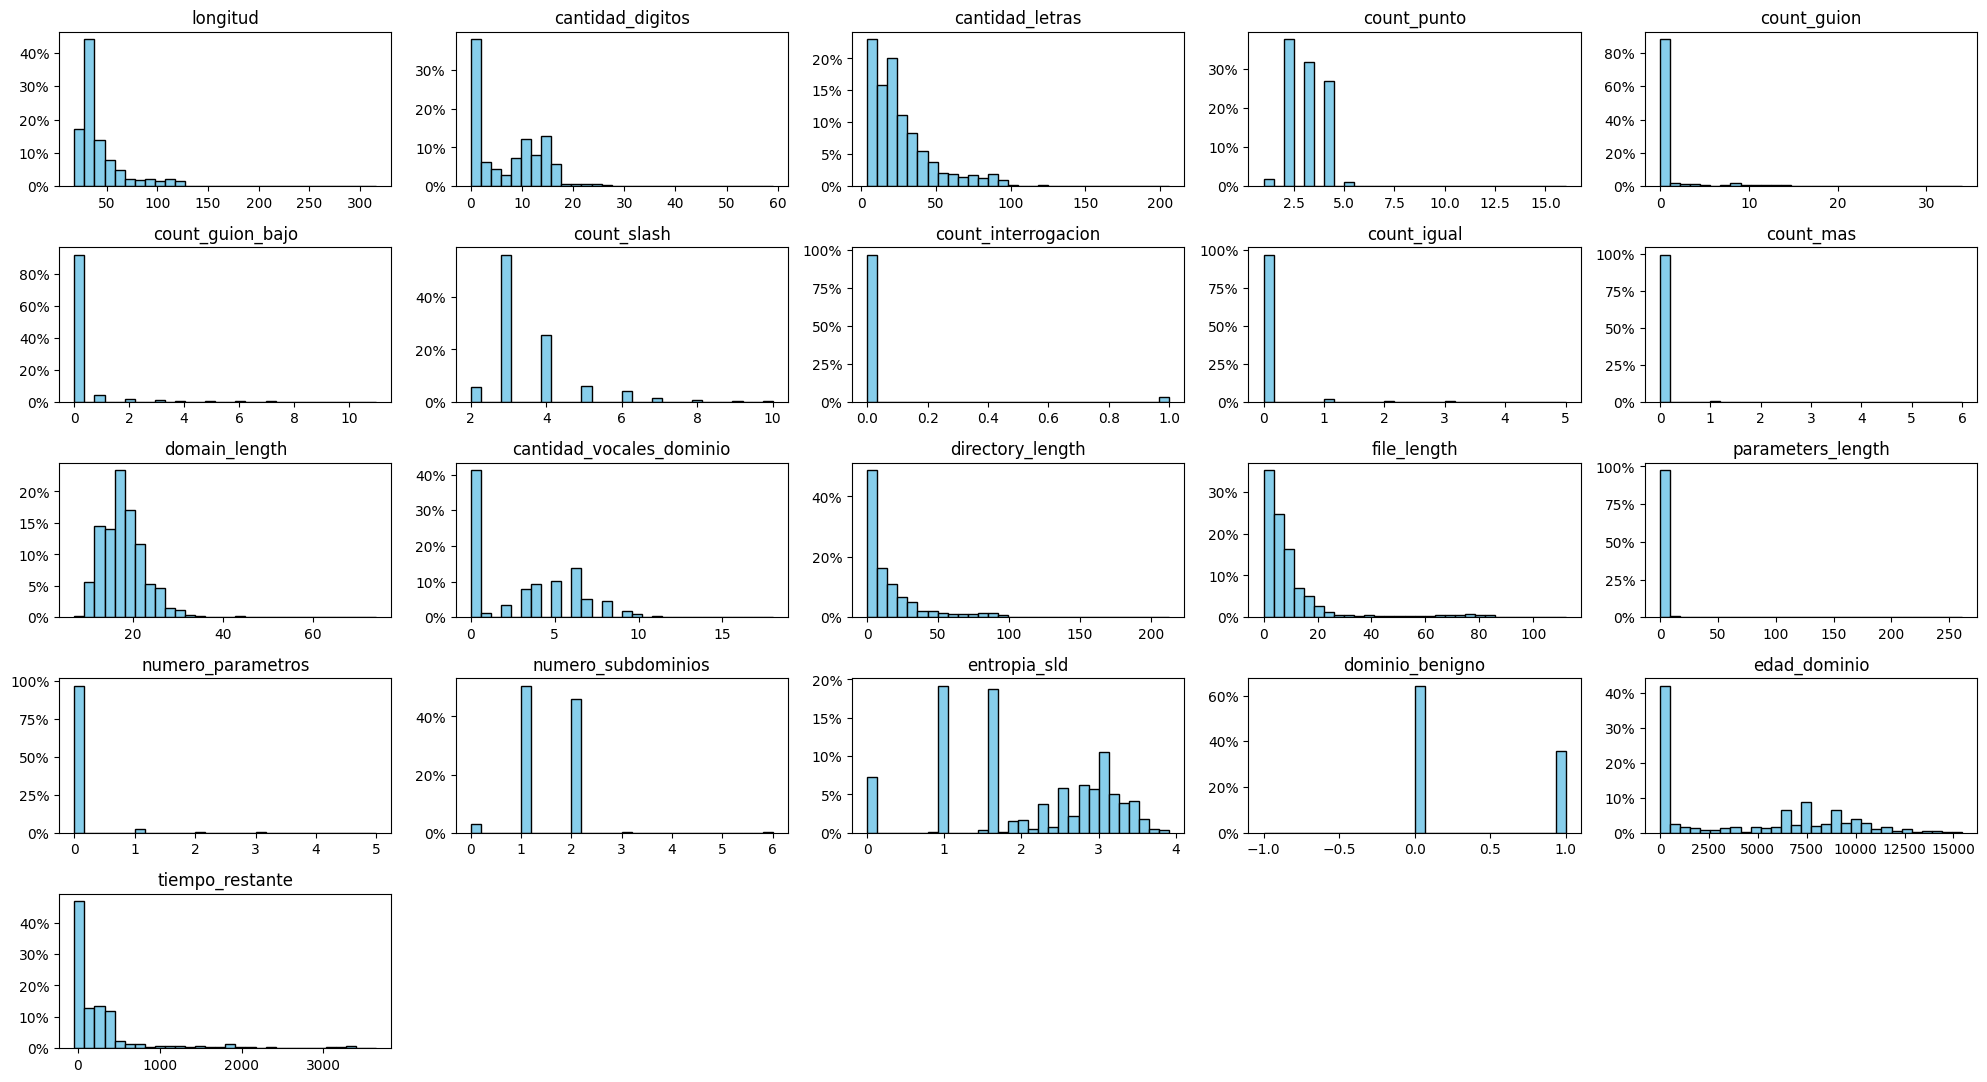
\includegraphics[width=\textwidth]{histogram1.png}
    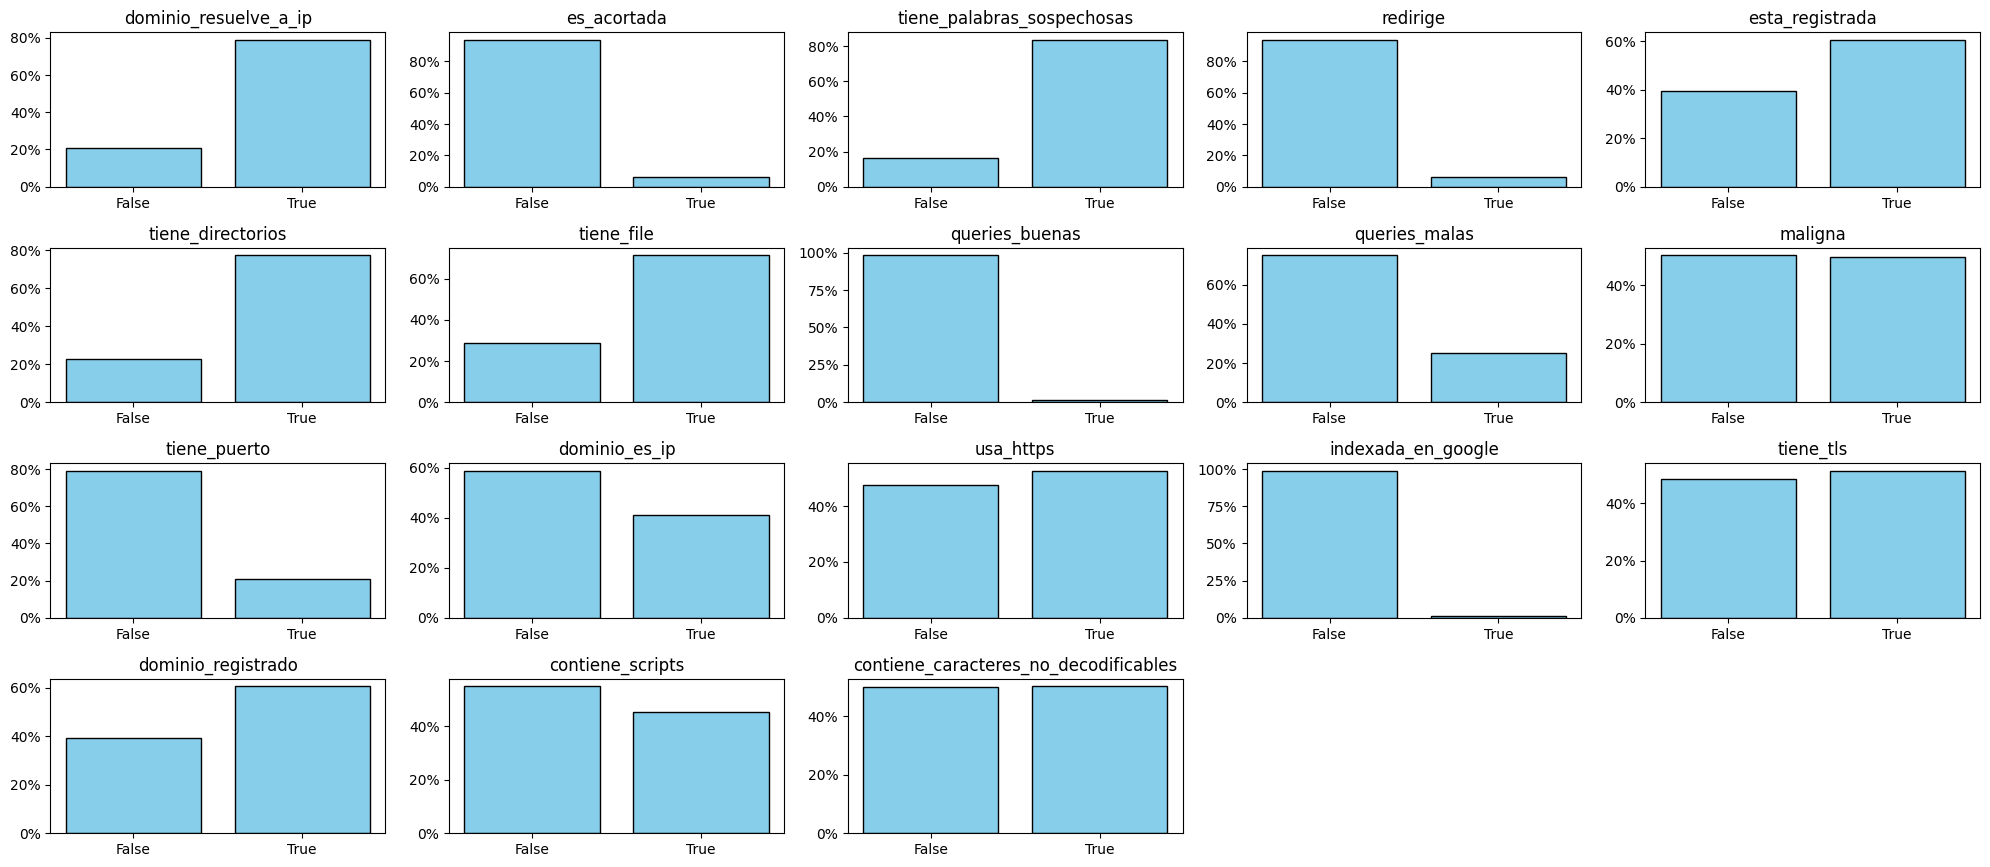
\includegraphics[width=\textwidth]{histogram2.png}
    \caption{Distribuciones de las características principales de las \glspl{url}.}
    \label{fig:histograms}
\end{figure}

\subsubsection*{Análisis de Correlación}

El análisis de correlación entre las características revela relaciones interesantes:

\begin{itemize}
    \item \textbf{Correlaciones Altas}: 
    Se observan correlaciones significativas entre características como si la \gls{url} esta registrada, la cantidad de letras y el uso de \gls{https}. Esto puede indicar que las \glspl{url} más largas y con más letras tienden a usar \gls{https}, lo cual puede estar relacionado con la seguridad de la \gls{url}.

    \item \textbf{Redundancia de Características}: 
    Algunas características muestran una alta correlación, lo que sugiere redundancia. Por ejemplo, la característica de uso de \gls{https} está altamente correlacionada con la longitud de la \gls{url} y la cantidad de letras, lo que llevó a la decisión de eliminar estas características en algunos modelos para evitar la multicolinealidad.
\end{itemize}

\begin{figure}[H]
    \centering
    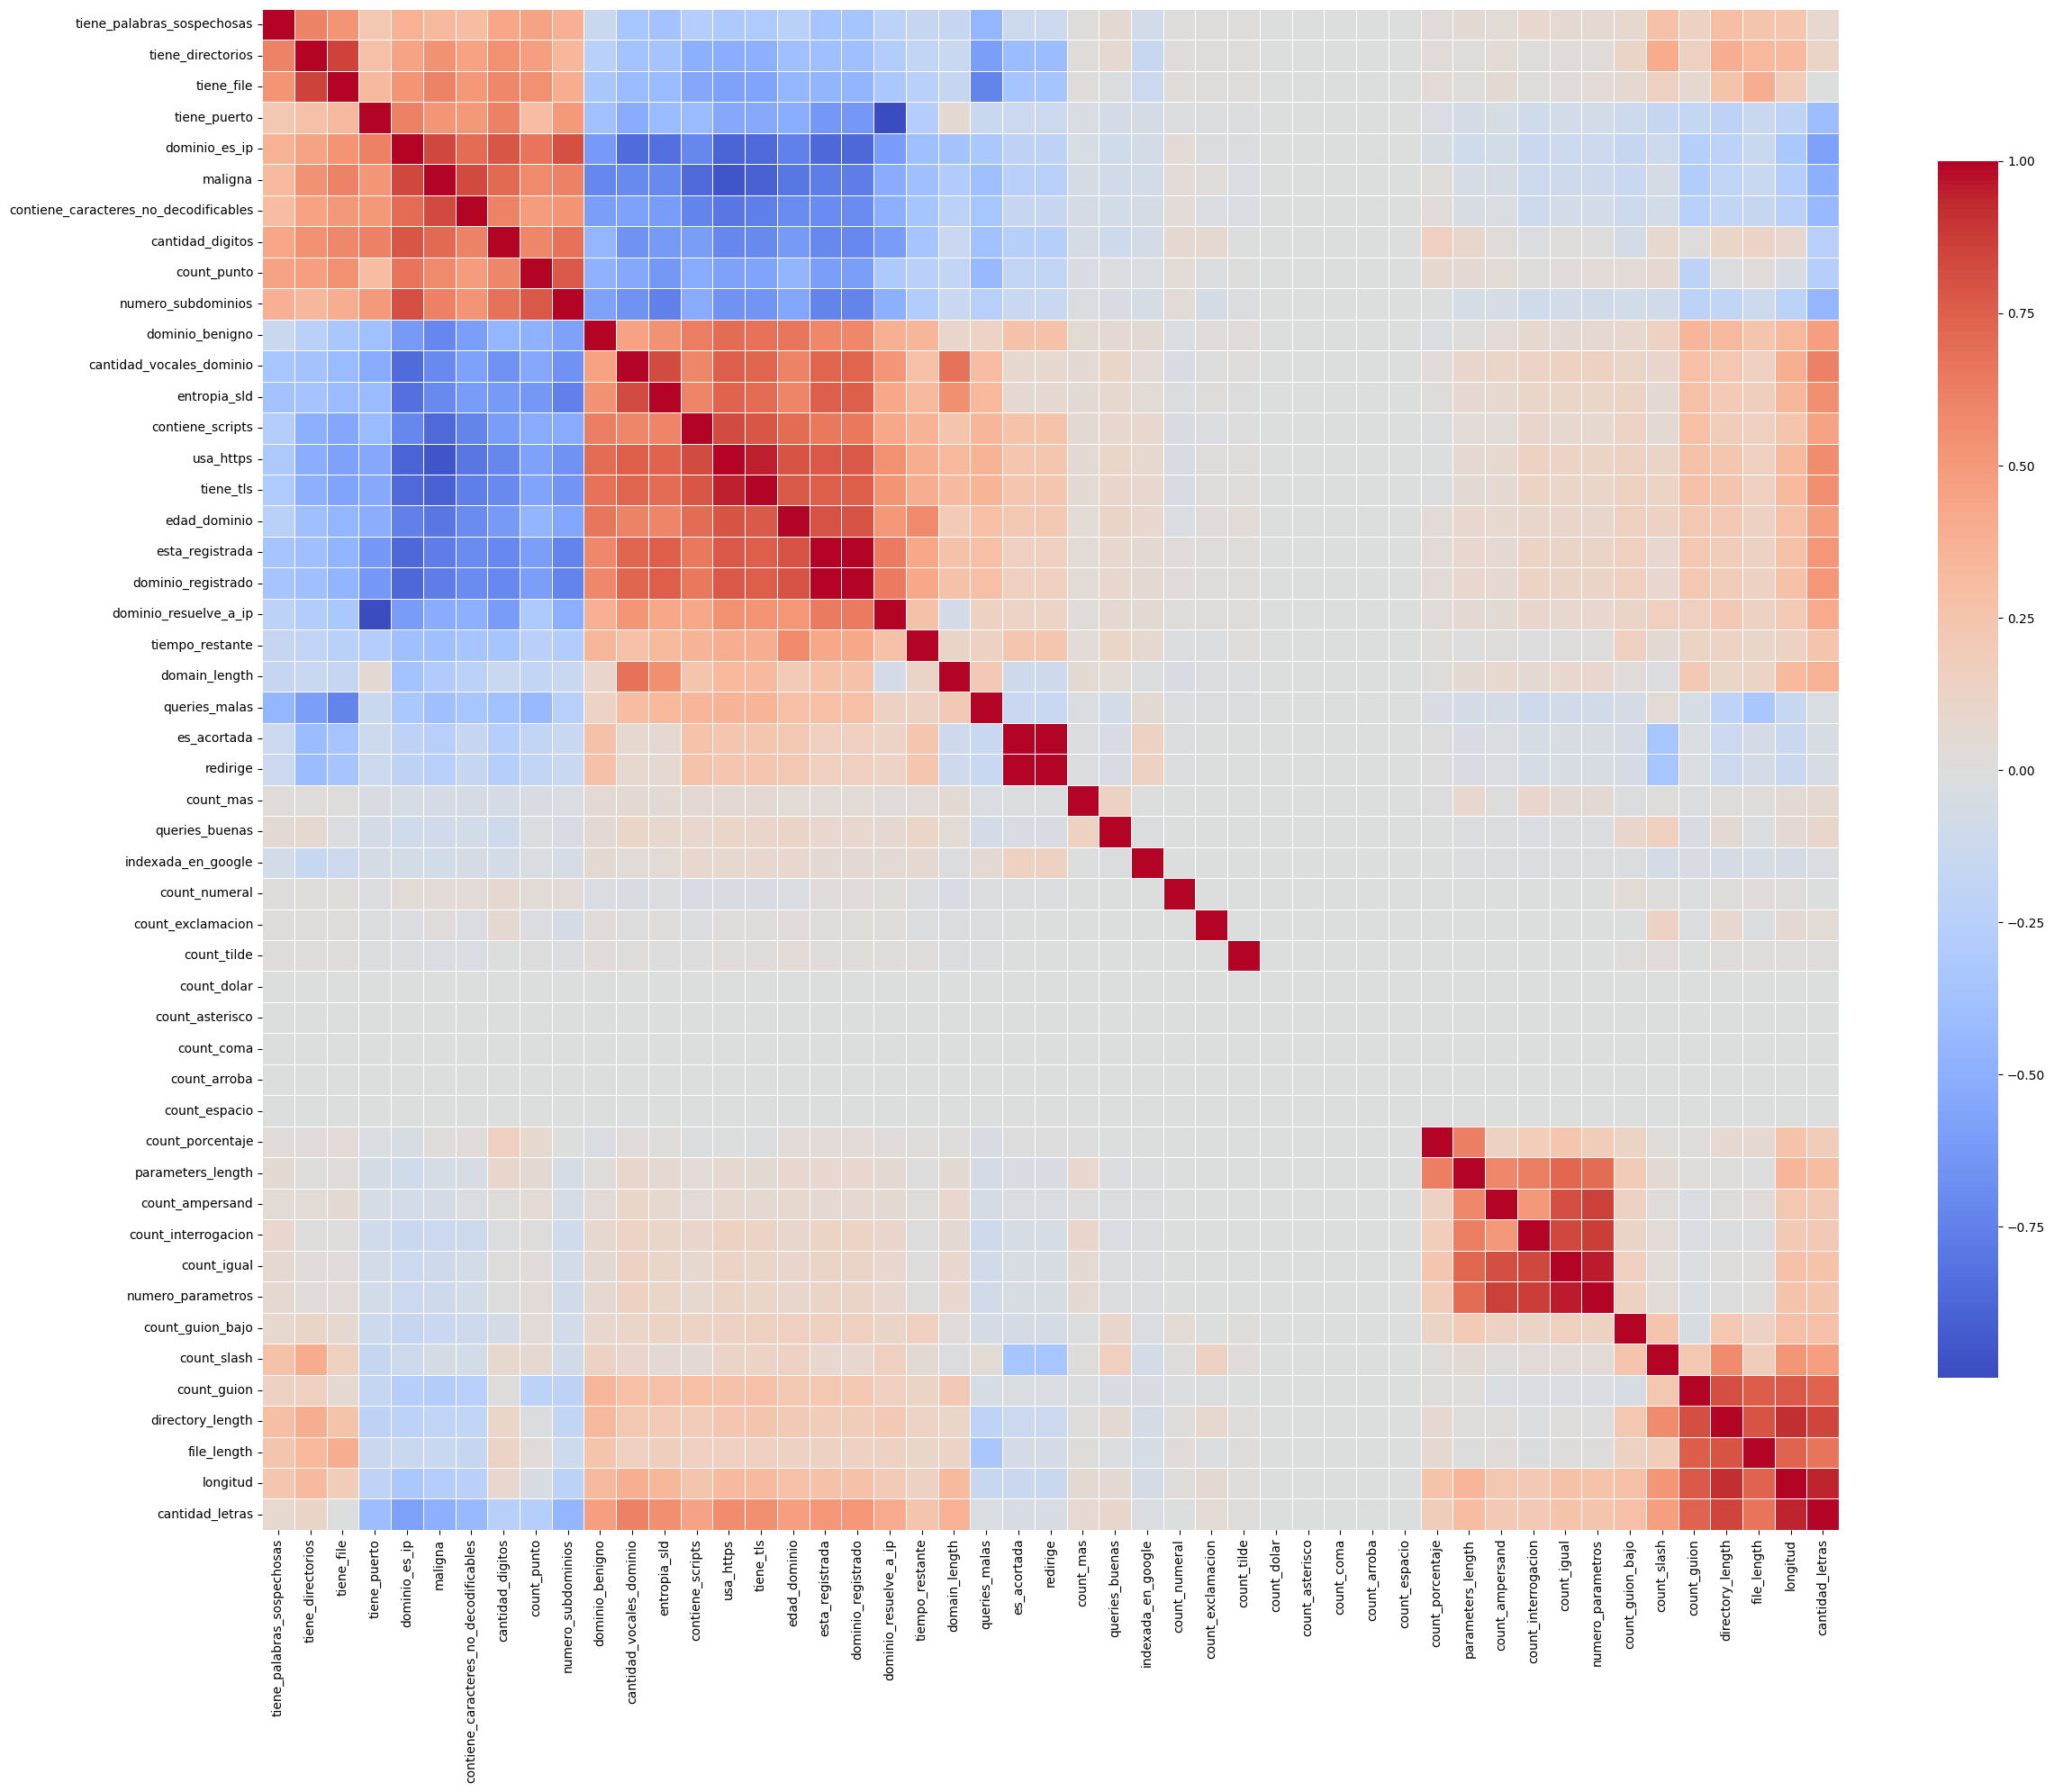
\includegraphics[width=\textwidth]{heatmap.png}
    \caption{Mapa de correlación entre las características extraídas de las \glspl{url}.}
    \label{fig:correlation_matrix}
\end{figure}












\subsection{Desempeño del Modelo de \textit{machine learning}}

En esta sección se presentan los resultados obtenidos de los diferentes modelos de \textit{machine learning} utilizados para la clasificación de \glspl{url} maliciosas y benignas, así como el análisis de su desempeño basado en las métricas de evaluación empleadas.

\subsubsection*{Modelos Evaluados}
Se evaluaron varios modelos de \textit{machine learning} utilizando la búsqueda de hiperparámetros con \textit{Grid Search} y \textit{Random Search}. Los modelos considerados incluyen:
\begin{itemize}
    \item Árbol de decisión
    \item \textit{Random Forest}
    \item \textit{K-Nearest Neighbors} (KNN)
    \item \textit{XGBoost}
    \item Máquina de Soporte Vectorial (SVM)
    \item \textit{LightGBM}
    \item \textit{Gradient Boosting}
    \item \textit{AdaBoost}
    \item Regresión Logística
\end{itemize}

Además, se utilizaron dos modelos de \textit{stacking} para combinar los resultados de múltiples clasificadores y mejorar el desempeño general.

\subsection{Métricas de Evaluación}
Las métricas de evaluación utilizadas fueron la precisión, el porcentaje de falsos positivos (FP) y el porcentaje de falsos negativos (FN). Estas métricas fueron seleccionadas debido a su importancia en la evaluación de modelos de clasificación, especialmente en el contexto de detección de \textit{phishing} y \glspl{url} maliciosas, donde es crucial minimizar tanto los falsos positivos como los falsos negativos.

\subsubsection*{Resultados de Validación y Prueba}

Las figuras \ref{fig:precision_validacion} y \ref{fig:precision_prueba} muestran la precisión de validación y prueba para los diferentes modelos evaluados. Los modelos \textit{Gradient boost} con \textit{Grid Search} y \textit{Random Search} demostraron ser los más precisos.

\begin{figure}[H]
    \centering
    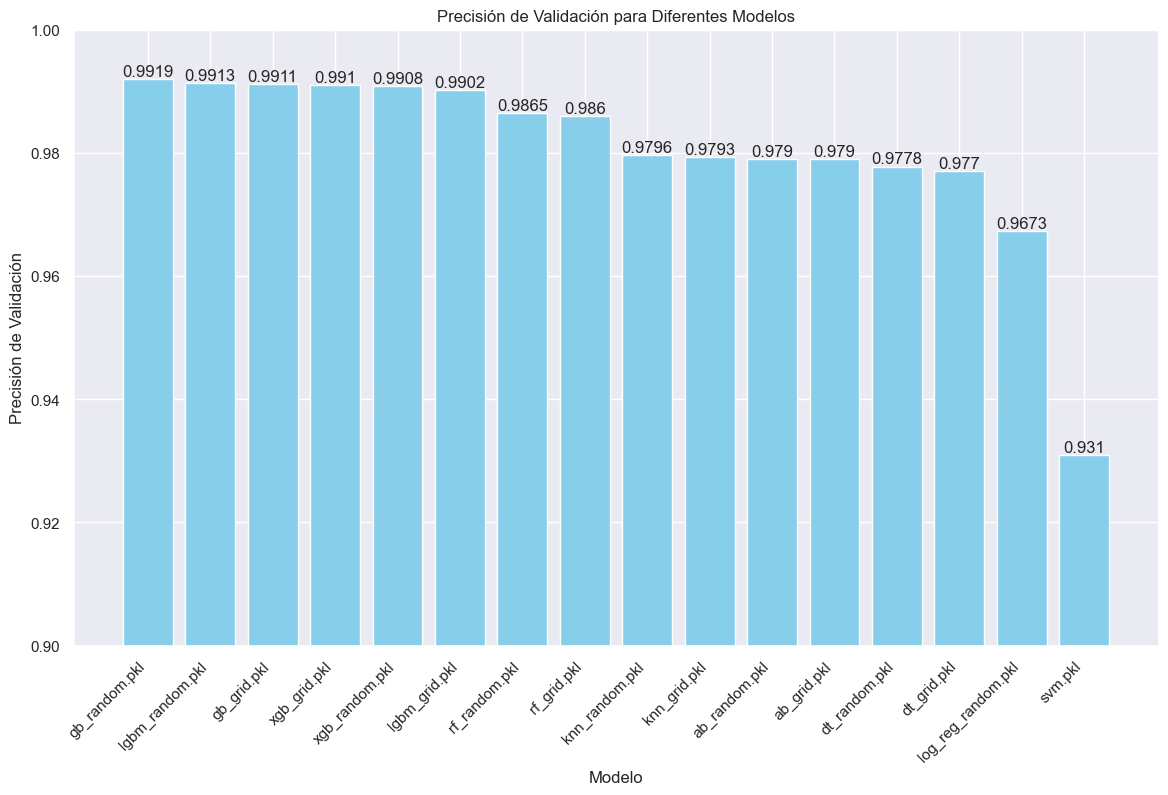
\includegraphics[width=0.8\textwidth]{precisionValidacion.png}
    \caption{Precisión de Validación para Diferentes Modelos}
    \label{fig:precision_validacion}
\end{figure}

\begin{figure}[H]
    \centering
    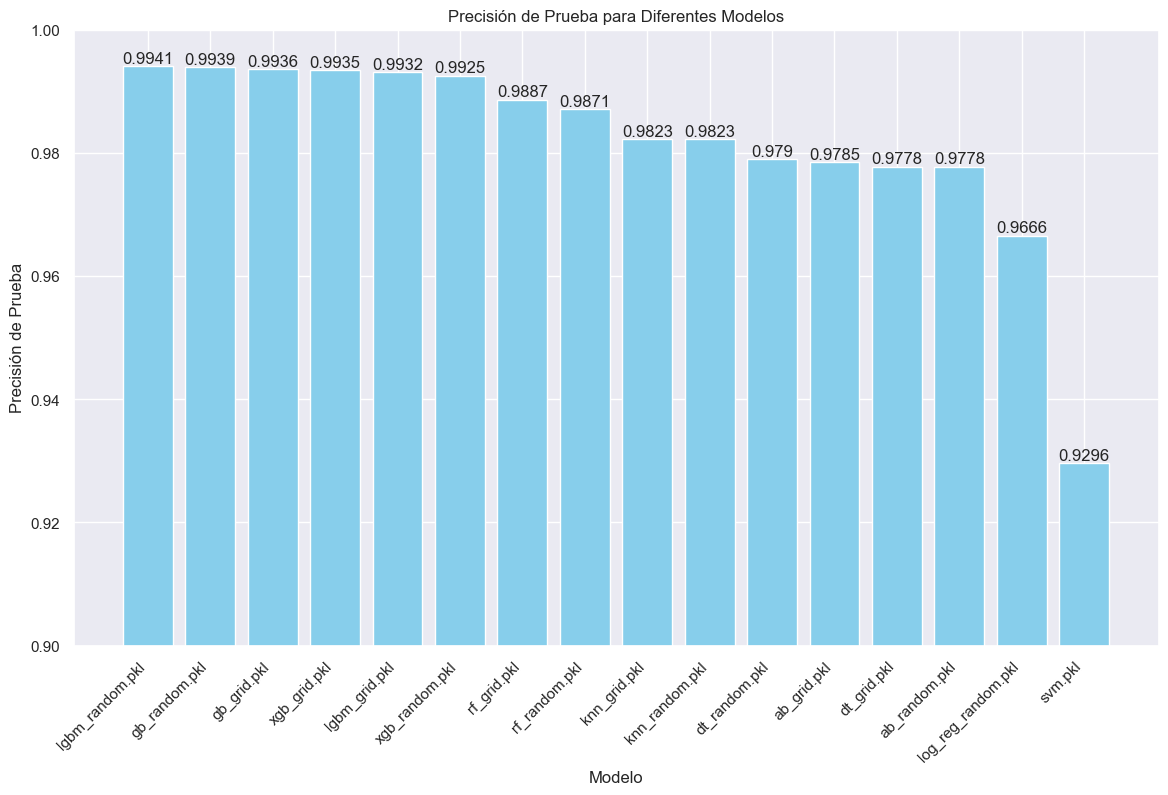
\includegraphics[width=0.8\textwidth]{precisionPrueba.png}
    \caption{Precisión de Prueba para Diferentes Modelos}
    \label{fig:precision_prueba}
\end{figure}

Las figuras \ref{fig:fp_validacion} y \ref{fig:fp_prueba} muestran el porcentaje de falsos positivos en validación y prueba, mientras que las figuras \ref{fig:fn_validacion} y \ref{fig:fn_prueba} muestran el porcentaje de falsos negativos en validación y prueba. Es evidente que el modelo SVM tuvo el mayor porcentaje de falsos positivos y negativos, mientras que los modelos basados en \textit{boosting} presentaron un mejor desempeño en términos de estas métricas.

\begin{figure}[H]
    \centering
    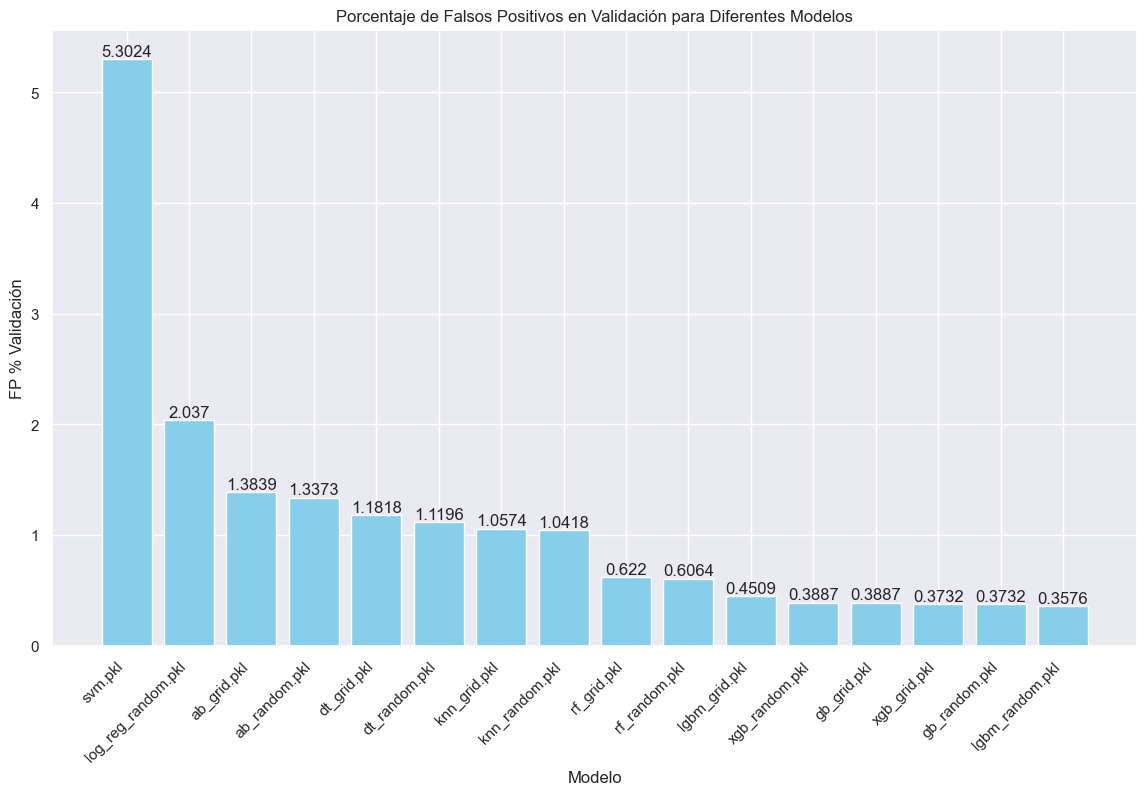
\includegraphics[width=0.8\textwidth]{positivosValidacion.png}
    \caption{Porcentaje de Falsos Positivos en Validación para Diferentes Modelos}
    \label{fig:fp_validacion}
\end{figure}

\begin{figure}[H]
    \centering
    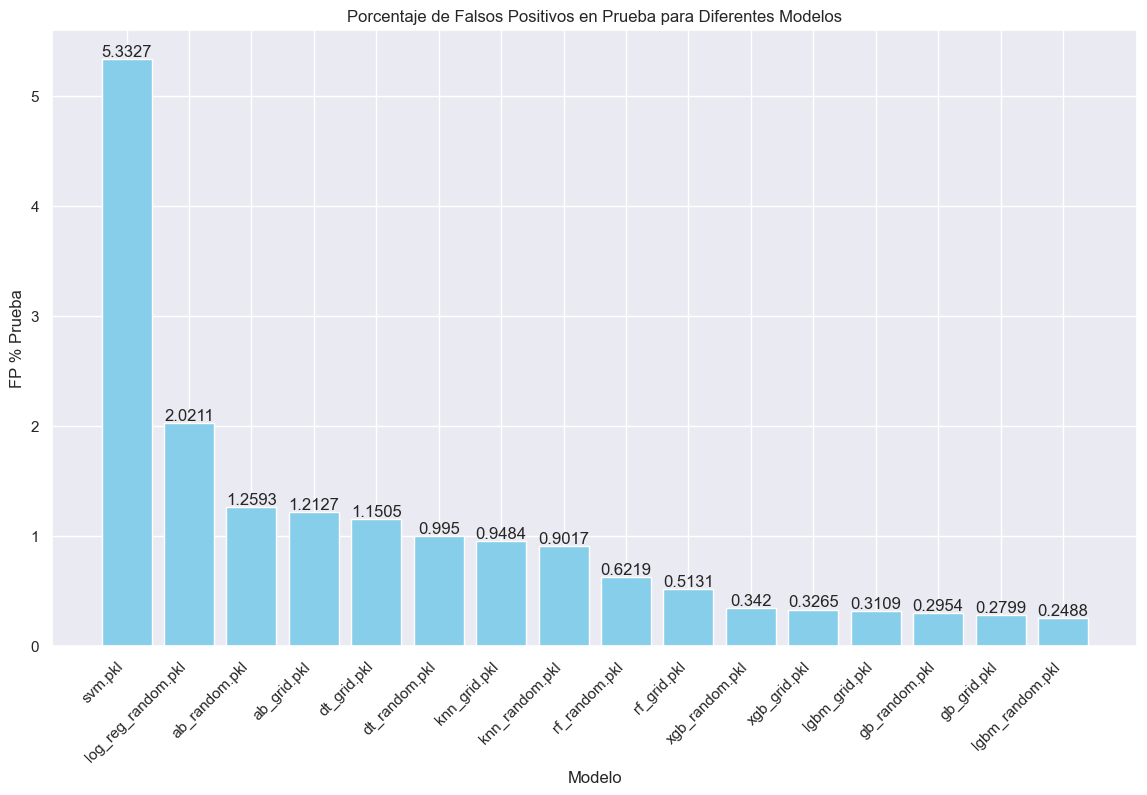
\includegraphics[width=0.8\textwidth]{positivosPrueba.png}
    \caption{Porcentaje de Falsos Positivos en Prueba para Diferentes Modelos}
    \label{fig:fp_prueba}
\end{figure}

\begin{figure}[H]
    \centering
    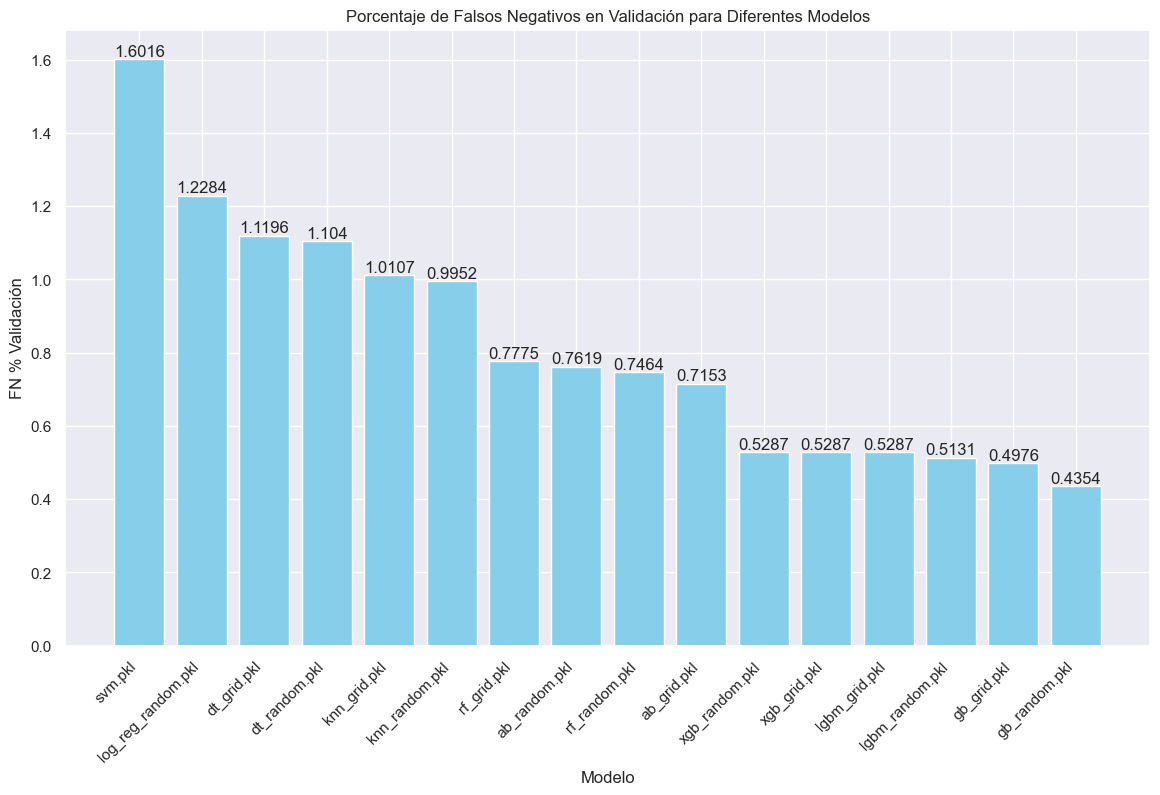
\includegraphics[width=0.8\textwidth]{negativosValidacion.png}
    \caption{Porcentaje de Falsos Negativos en Validación para Diferentes Modelos}
    \label{fig:fn_validacion}
\end{figure}

\begin{figure}[H]
    \centering
    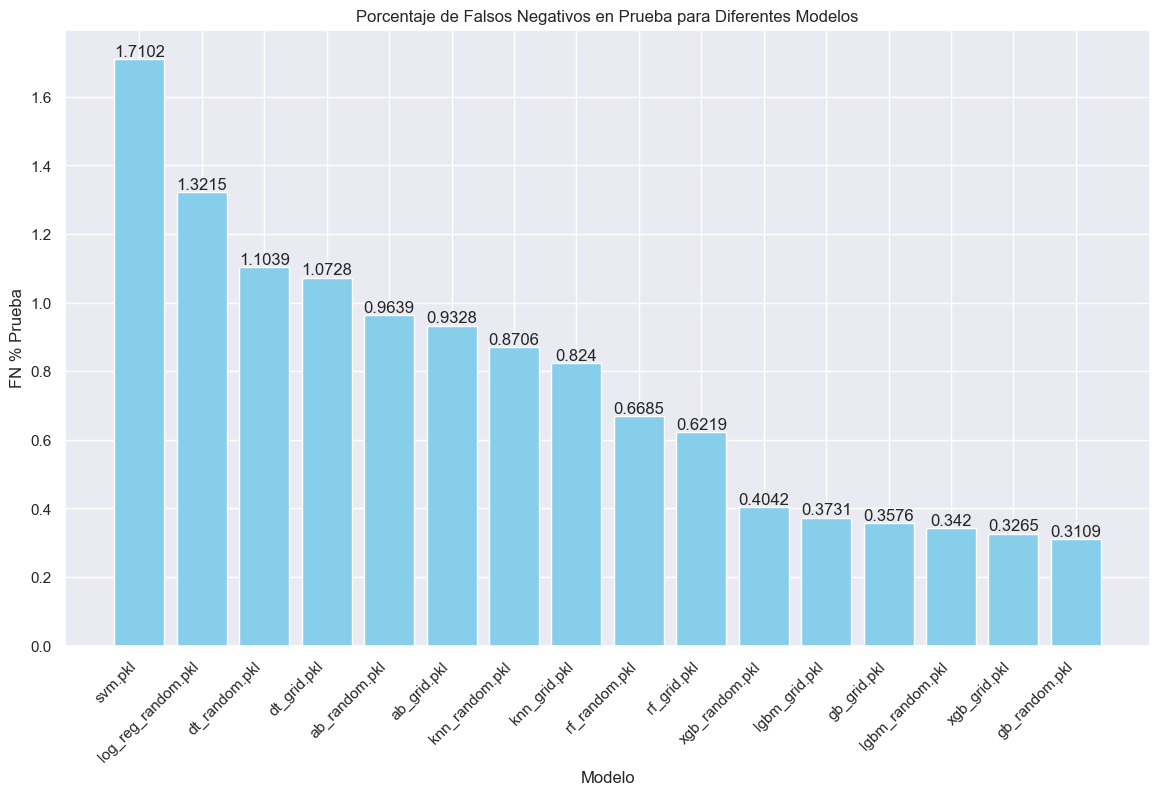
\includegraphics[width=0.8\textwidth]{negativosPrueba.png}
    \caption{Porcentaje de Falsos Negativos en Prueba para Diferentes Modelos}
    \label{fig:fn_prueba}
\end{figure}

\subsubsection*{Modelos de \textit{Stacking}}

El primer modelo de \textit{stacking} combinado mostró una precisión de validación del 98.78\% y una precisión de prueba del 99.00\%, con falsos positivos y falsos negativos inferiores al 0.6\%. El segundo modelo de \textit{stacking}, que utilizó un conjunto diferente de características y clasificadores base, logró una precisión de validación y prueba del 99.17 y 99.28\% respectivamente, con falsos positivos y negativos de apenas 0.40\%.

\begin{table}[H]
    \centering
    \begin{tabular}{lcc}
        \hline
        \textbf{Modelo} & \textbf{Precisión Validación (\%)} & \textbf{Precisión Prueba (\%)} \\
        \hline
        \textit{Stacking 1} & 98.78 & 99.00 \\
        \textit{Stacking 2} & 99.17 & 99.28 \\
        \hline
    \end{tabular}
    \caption{Resultados de Precisión para los Modelos de \textit{Stacking}}
    \label{tab:stacking_results}
\end{table}

El alto desempeño de los modelos de \textit{stacking} destaca su capacidad para combinar las fortalezas de múltiples clasificadores, resultando en un sistema más robusto y preciso para la detección de \glspl{url} maliciosas.


A continuación, se presenta una tabla comparativa de los modelos ordenados por su precisión en el conjunto de prueba:

\begin{table}[H]
    \centering
    \begin{tabular}{lccc}
        \hline
        \textbf{Modelo} & \textbf{Precisión Prueba (\%)} & \textbf{FP Prueba (\%)} & \textbf{FN Prueba (\%)} \\
        \hline
        \textit{Stacking 2} & 99.28 & 0.40 & 0.31 \\
        \textit{Stacking 1} & 99.00 & 0.42 & 0.58 \\
        \textit{xgb\_grid} & 98.94 & 0.46 & 0.6 \\
        \textit{xgb\_random} & 98.83 & 0.50 & 0.66 \\
        \textit{gb\_random} & 99.04 & 0.46 & 0.50 \\
        \textit{gb\_grid} & 98.92 & 0.46 & 0.62 \\
        \textit{log\_reg\_random} & 96.89 & 1.72 & 1.39 \\
        \textit{rf\_grid} & 98.86 & 0.51 & 0.62 \\
        \textit{rf\_random} & 98.70 & 0.62 & 0.67 \\
        \textit{lgbm\_random} & 98.96 & 0.46 & 0.58 \\
        \textit{lgbm\_grid} & 98.88 & 0.52 & 0.60 \\
        \textit{dt\_grid} & 97.77 & 1.15 & 1.07 \\ 
        \textit{dt\_random} & 97.90 & 1.00 & 1.10 \\ 
        \textit{knn\_random} & 97.22 & 1.29 & 1.49 \\
        \textit{knn\_grid} & 97.22 & 1.33 & 1.45 \\
        \textit{ab\_grid} & 98.09 & 1.04 & 0.87 \\
        \textit{ab\_random} & 98.00 & 1.16 & 0.83 \\
        \textit{svm} &  93.01& 5.22 & 1.76 \\
        \hline
    \end{tabular}
    \caption{Comparación de Modelos Ordenados por Precisión en Prueba}
    \label{tab:model_comparison}
\end{table}
\subsection{Resultados de la implementación en tiempo real}

\subsection*{Evaluación del Plugin}

\subsubsection*{Descripción General}
El plugin desarrollado, denominado \textit{URL Analyzer}, tiene como objetivo identificar y notificar a los usuarios sobre la naturaleza maliciosa o benigna de las \glspl{url} que visitan. Se activa automáticamente al ingresar a una página web y ofrece la opción de análisis manual a través de un botón en la extensión.

\subsubsection*{Funcionamiento}
El plugin realiza un análisis enviando una solicitud POST a un servidor Flask que aloja un modelo de \textit{Machine Learning} previamente entrenado. Este modelo evalúa las características de la \gls{url} y determina si es maliciosa o benigna. El resultado del análisis se muestra en un popup que informa al usuario sobre la seguridad de la \gls{url}, incluyendo una estimación de la probabilidad de que la \gls{url} sea maliciosa. El tiempo promedio de respuesta del análisis es de aproximadamente 5 segundos.

\subsubsection*{Pruebas de Evaluación}
Para evaluar la eficacia del plugin, se realizaron pruebas en diferentes escenarios con \glspl{url} benignas y maliciosas. A continuación, se presentan los resultados de estas pruebas.

\subsubsection*{Caso de Prueba 1: URL Benigna (Facebook)}
\textbf{Descripción:}
El plugin fue evaluado utilizando la \gls{url} de Facebook, una plataforma de redes sociales ampliamente reconocida y segura.



\textbf{Resultado:}
El análisis indicó que la \gls{url} \url{https://www.facebook.com/} es benigna, con una probabilidad del 0.33\% de ser maliciosa.

\begin{figure}[H]
    \centering
    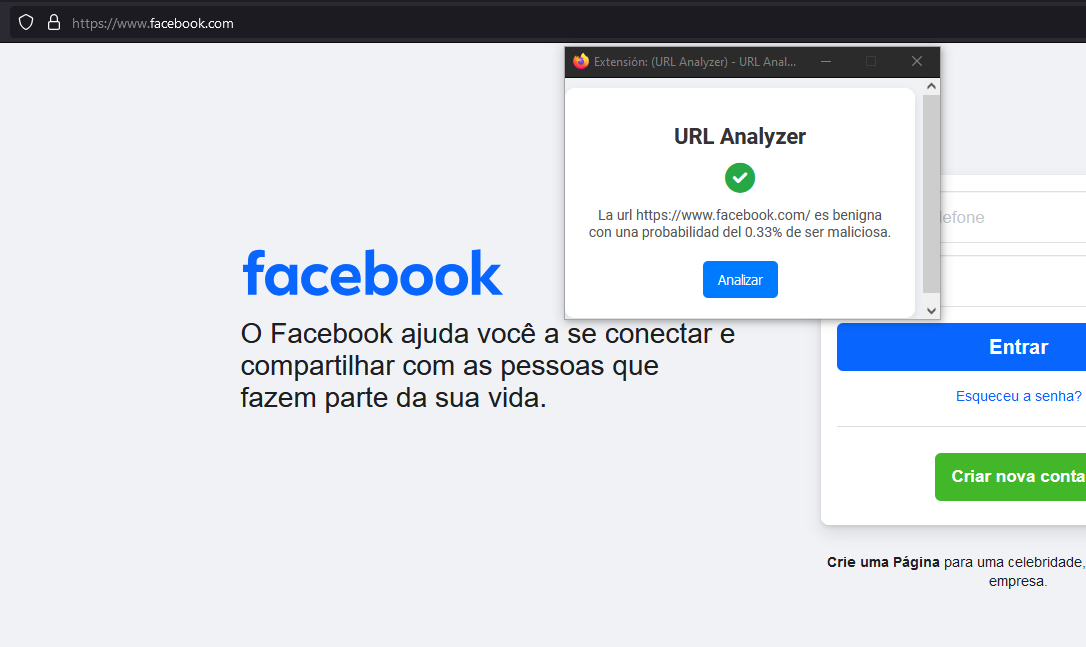
\includegraphics[width=0.7\textwidth]{image1.png}
    \caption{Análisis de la URL de Facebook.}
    \label{fig:facebook}
\end{figure}

\subsubsection*{Caso de Prueba 2: URL Maliciosa (Clon de Discord)}
\textbf{Descripción:}
Se utilizó una \gls{url} que imita la página de Discord, diseñada para engañar a los usuarios.

\textbf{Resultado:}
El análisis mostró que la \gls{url} \url{https://discord.zhangxinhe.com/} es maliciosa, con una probabilidad del 87.31\% de ser maliciosa.



\begin{figure}[H]
    \centering
    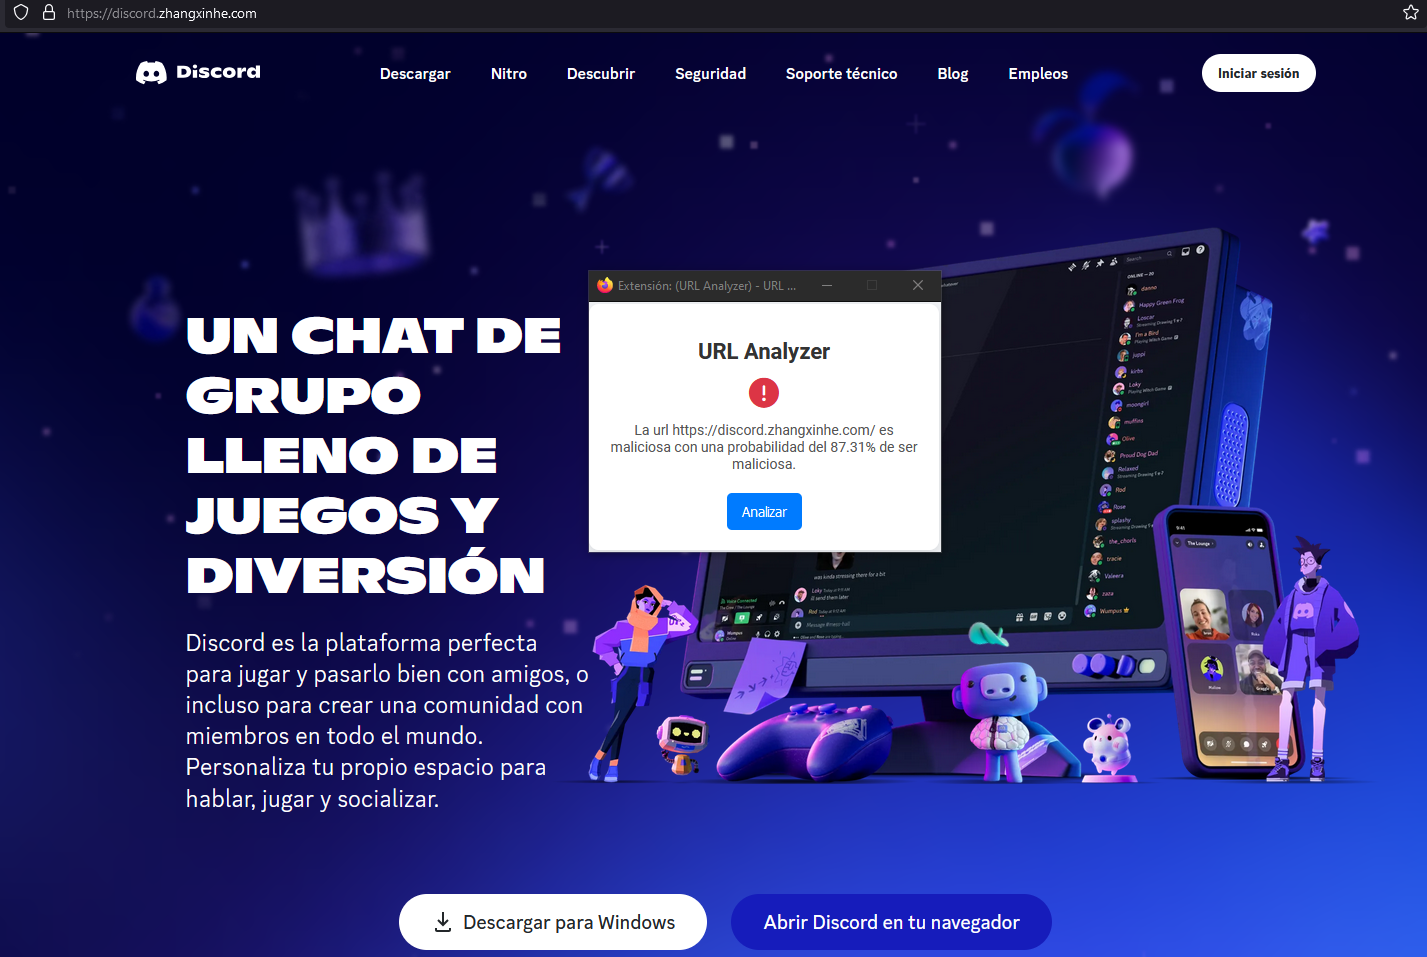
\includegraphics[width=0.7\textwidth]{image2.png}
    \caption{Análisis de una URL maliciosa clon de Discord.}
    \label{fig:discord_malicious}
\end{figure}

\subsubsection*{Caso de Prueba 3: URL Benigna (Discord)}
\textbf{Descripción:}
El plugin fue evaluado con la \gls{url} oficial de Discord, un servicio legítimo de chat y comunicación.

\textbf{Resultado:}
El análisis indicó que la \gls{url} \url{https://discord.com/} es benigna, con una probabilidad del 0.33\% de ser maliciosa.

\begin{figure}[H]
    \centering
    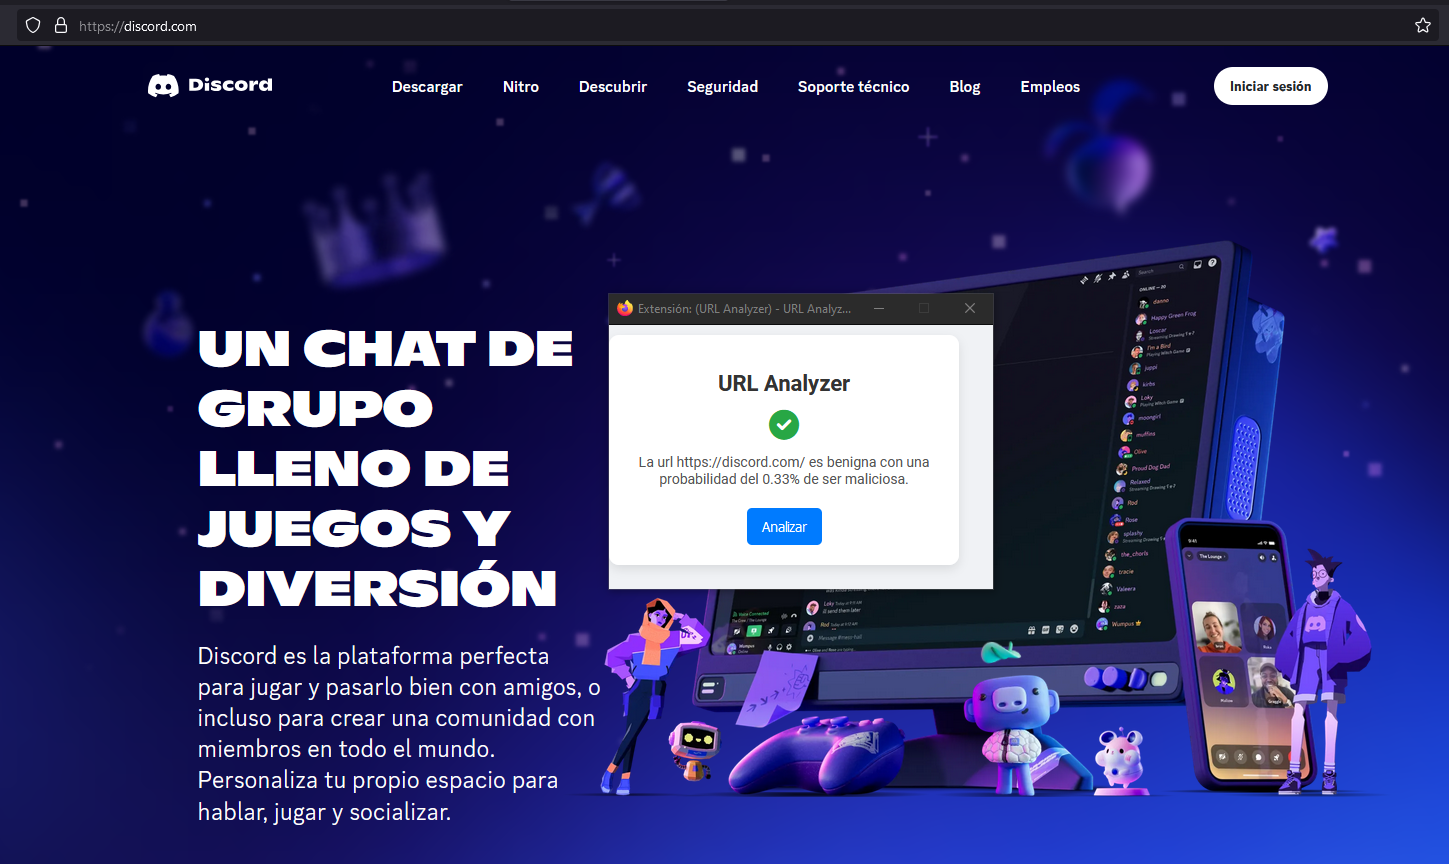
\includegraphics[width=0.7\textwidth]{image3.png}
    \caption{Análisis de la URL oficial de Discord.}
    \label{fig:discord}
\end{figure}

\subsubsection*{Caso de Prueba 4: URL Benigna (YouTube)}
\textbf{Descripción:}
Se probó el plugin con la \gls{url} de YouTube, una plataforma de videos conocida y segura.

\textbf{Resultado:}
El análisis mostró que la \gls{url} \url{https://www.youtube.com/} es benigna, con una probabilidad del 0.33\% de ser maliciosa.

\begin{figure}[H]
    \centering
    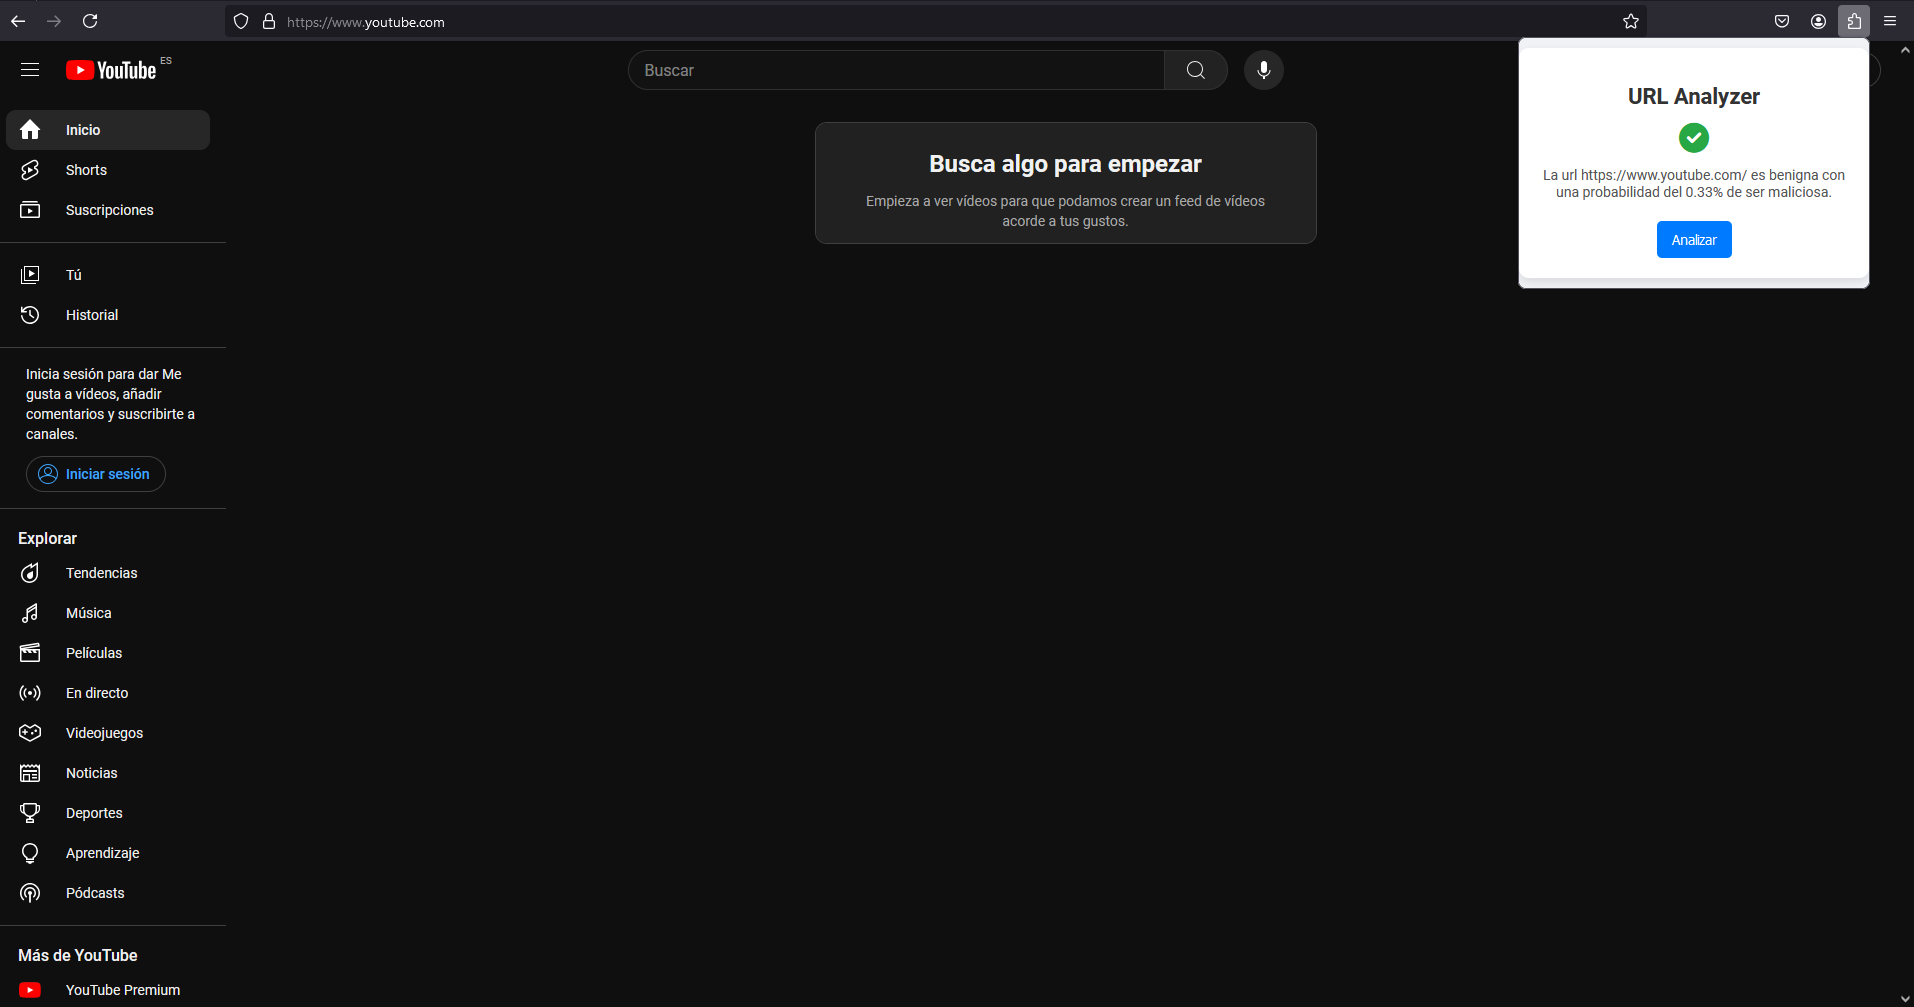
\includegraphics[width=0.7\textwidth]{image4.png}
    \caption{Análisis de la URL de YouTube.}
    \label{fig:youtube}
\end{figure}

\subsubsection*{Caso de Prueba 5: URL Maliciosa (Proxy de Discord)}
\textbf{Descripción:}
Se utilizó una \gls{url} que actúa como un proxy de Discord, diseñada para engañar a los usuarios.

\textbf{Resultado:}
El análisis indicó que la \gls{url} \url{https://discord-proxy.tassadar2002.workers.dev/} es maliciosa, con una probabilidad del 91.77\% de ser maliciosa.

\begin{figure}[H]
    \centering
    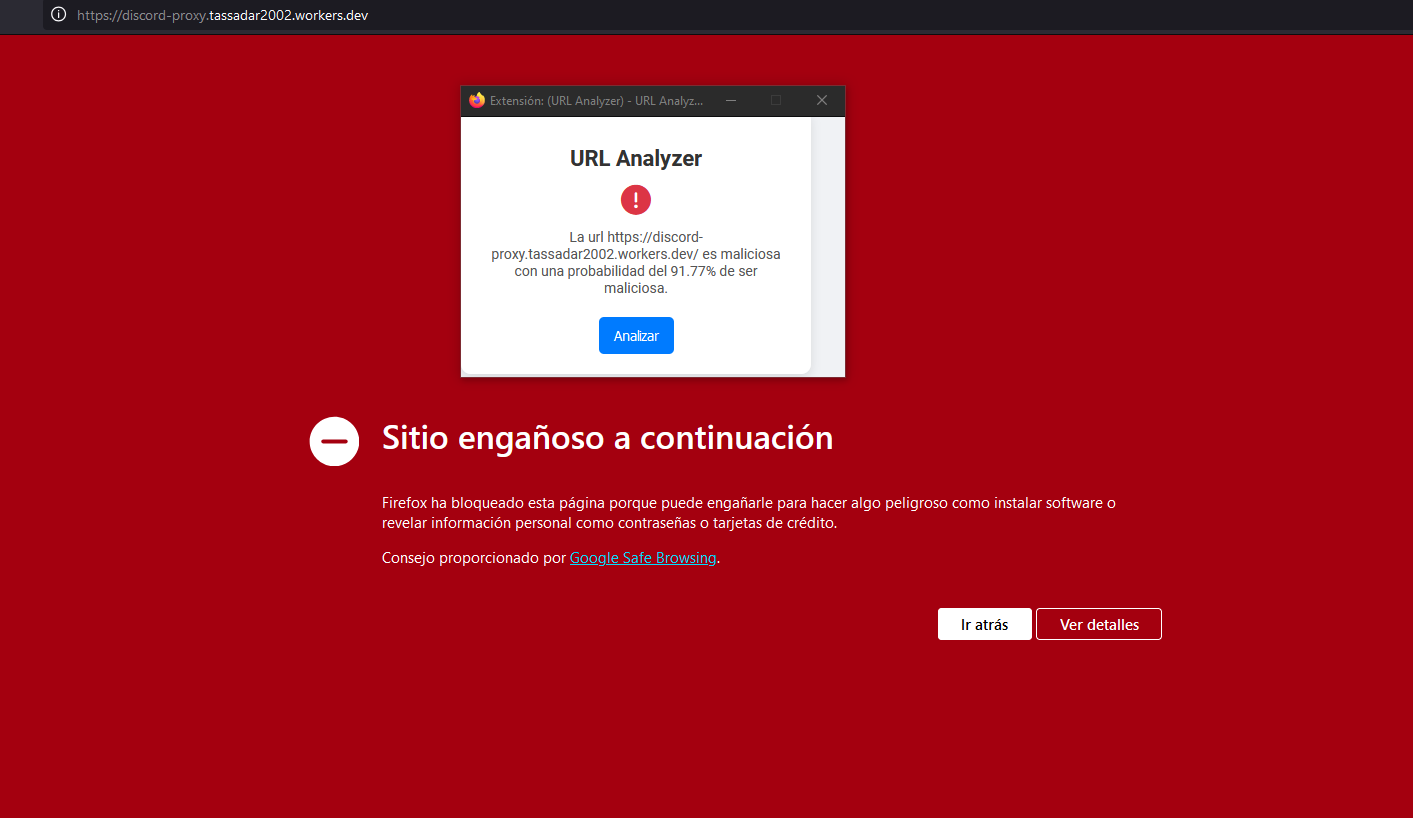
\includegraphics[width=0.7\textwidth]{image5.png}
    \caption{Análisis de una URL maliciosa proxy de Discord.}
    \label{fig:discord_proxy}
\end{figure}

\textbf{Nota:}
El navegador Firefox también detectó esta \gls{url} como maliciosa antes de que el plugin realizara su análisis, proporcionando una segunda capa de seguridad.


\subsubsection*{Caso de Prueba 6: URL Maliciosa Ignorando Advertencia del Navegador}
\textbf{Descripción:}
Se utilizó la misma URL maliciosa del Caso de Prueba 5, pero se ignoró la advertencia del navegador para entrar en la página.

\textbf{Resultado:}
El plugin siguió mostrando que la \gls{url} \url{https://discord-proxy.tassadar2002.workers.dev/} es maliciosa, con una probabilidad del 91.77\% de ser maliciosa.

\begin{figure}[H]
    \centering
    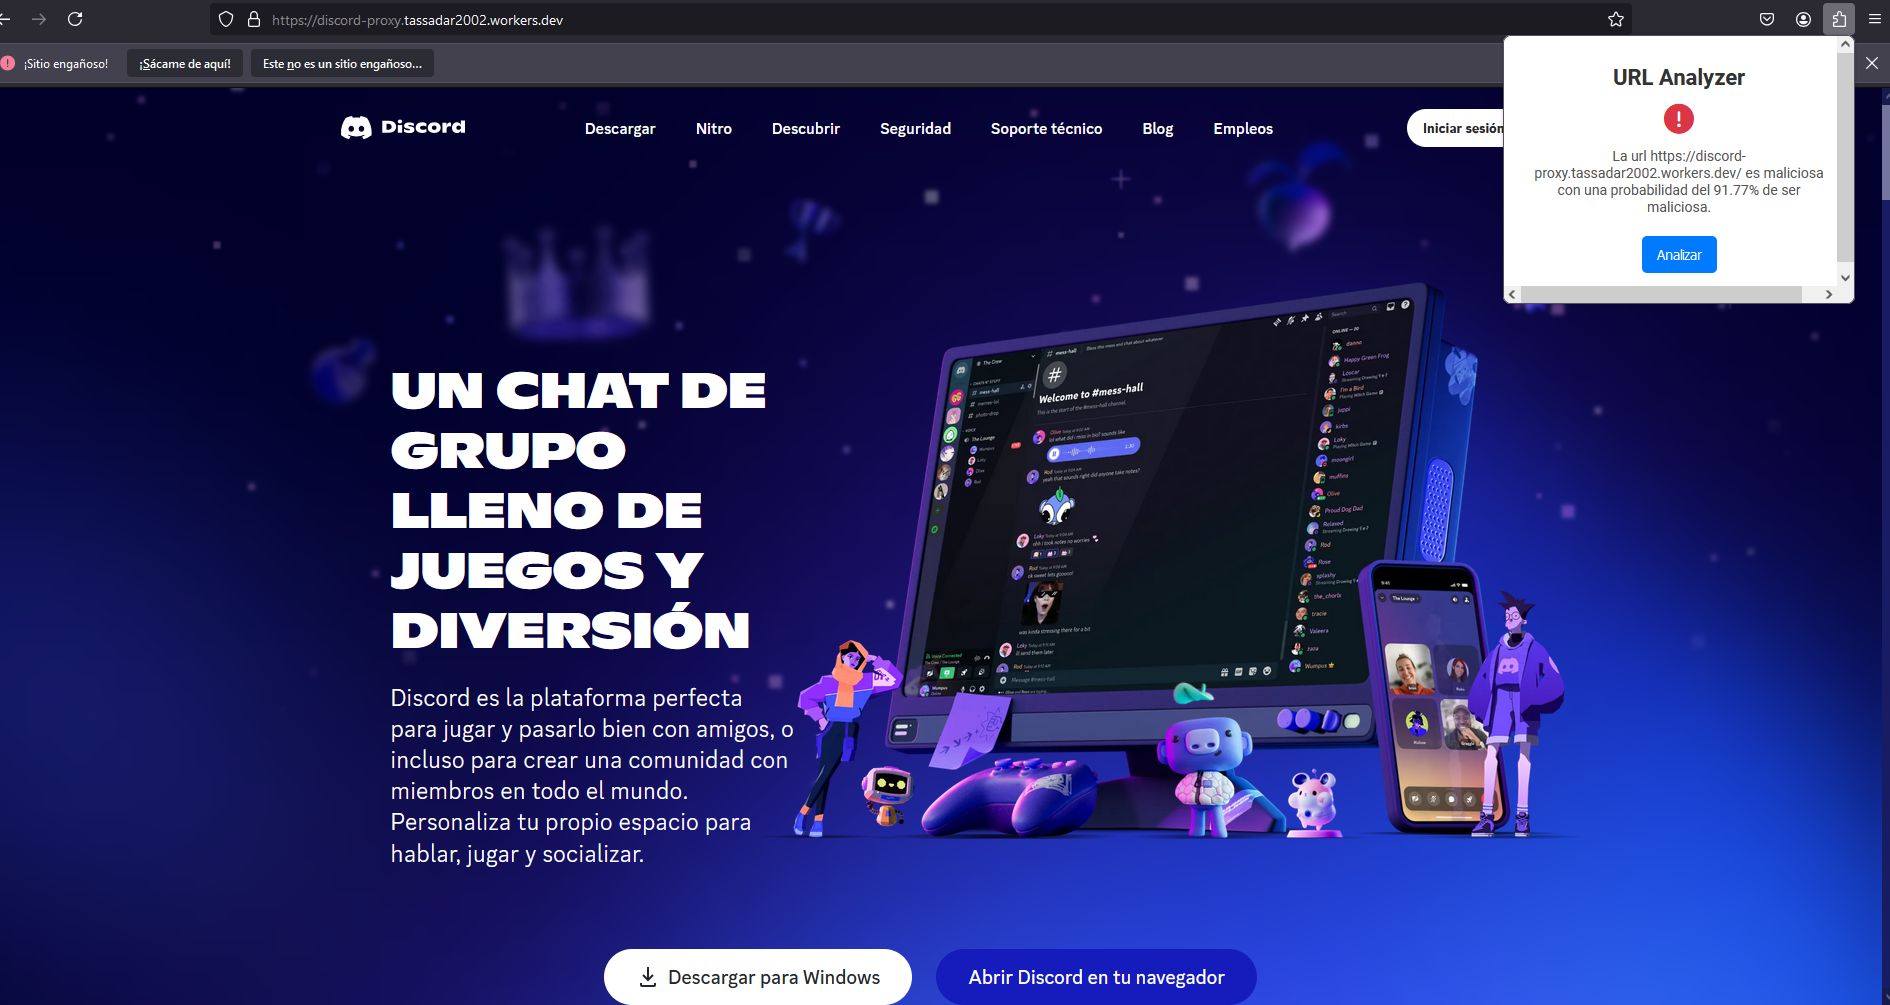
\includegraphics[width=0.7\textwidth]{image6.png}
    \caption{Análisis de una URL maliciosa ignorando la advertencia del navegador.}
    \label{fig:discord_proxy_ignored}
\end{figure}


\subsubsection*{Consideraciones Adicionales}
\begin{itemize}
    \item \textbf{Tiempo de Respuesta:} El tiempo promedio de análisis es de 5 segundos, lo que es razonable dado el nivel de análisis realizado.
    \item \textbf{Precisión:} El modelo de \textit{Machine Learning} utilizado por el plugin ha mostrado una alta precisión en la identificación de \glspl{url} maliciosas y benignas durante las pruebas.
    \item \textbf{Usabilidad:} La interfaz del plugin es intuitiva y fácil de usar, con notificaciones claras y accesibles para el usuario.
\end{itemize}

Para futuras mejoras, se podría considerar la optimización del tiempo de respuesta y la incorporación de funcionalidades adicionales basadas en feedback de los usuarios.

\subsection{Evaluación del Dashboard}

\subsection*{Descripción General}

El dashboard desarrollado con Streamlit, denominado \textit{Dashboard de URLs}, está diseñado para analizar y visualizar características de URLs almacenadas en la base de datos. El dashboard tiene dos partes principales:

\begin{enumerate}
    \item \textbf{Análisis de URL:} Permite a los usuarios ingresar una URL para obtener un informe detallado de sus características, incluyendo si es maligna o no. Este proceso toma aproximadamente 5 segundos.
    \item \textbf{Dashboard de Estadísticas:} Muestra diversas gráficas e informes sobre las características de las URLs almacenadas en la base de datos, ofreciendo una visión detallada y rápida de los datos ya extraídos.
\end{enumerate}

\subsection*{Funcionamiento}


\begin{figure}[H]
    \centering
    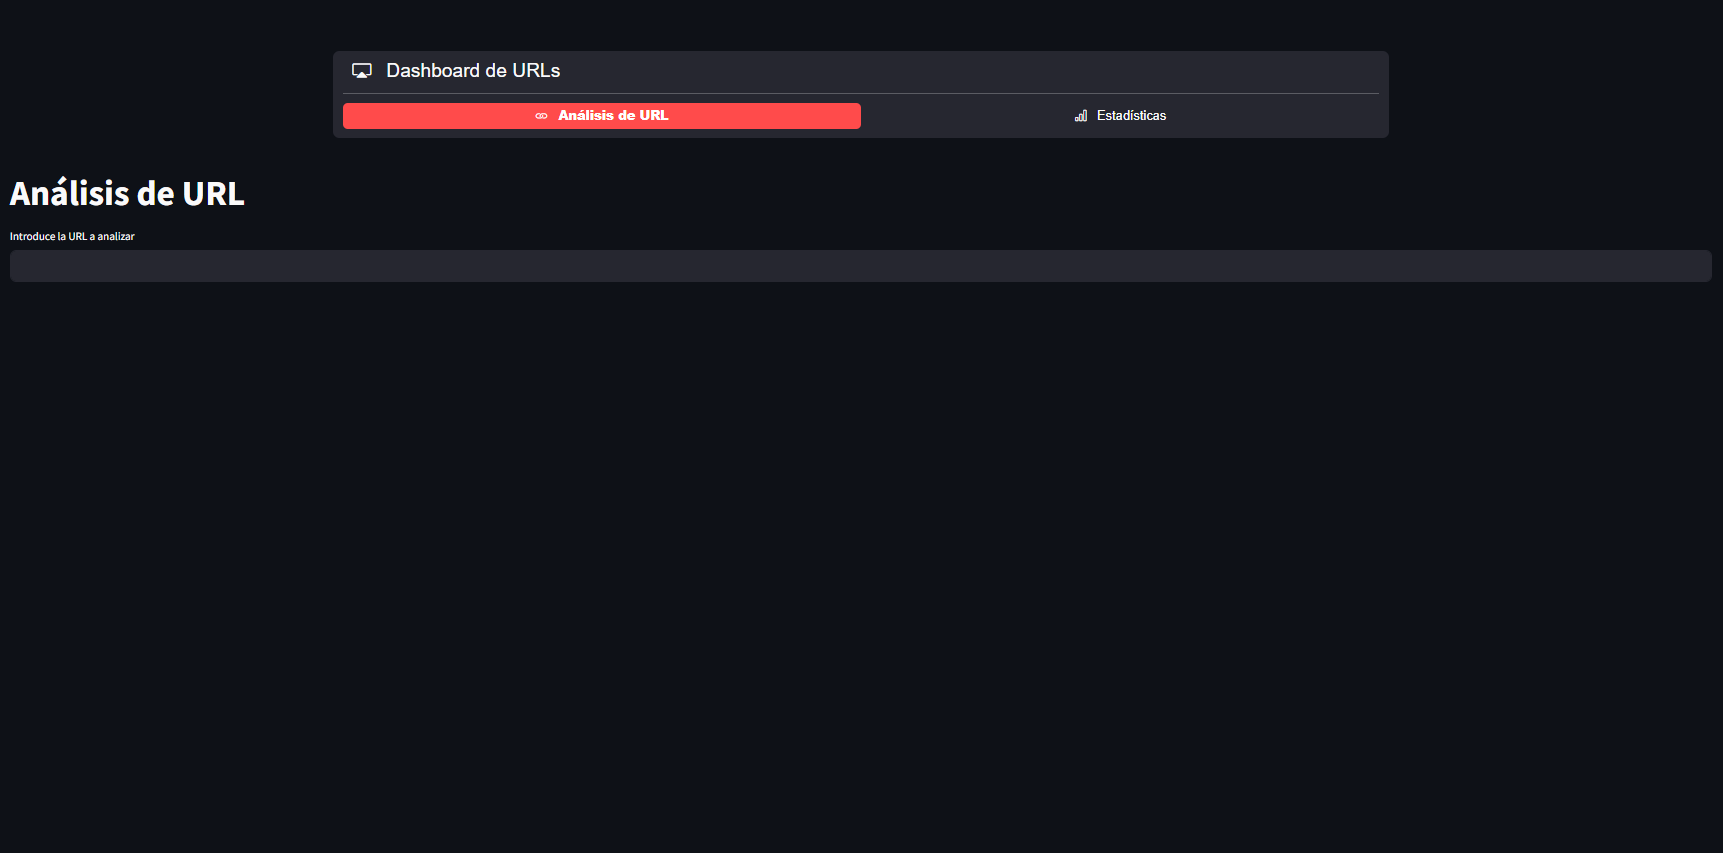
\includegraphics[width=\textwidth]{interfazAnalisis.png}
    \caption{Interfaz de análisis de URL}
\end{figure}

La primera parte del dashboard permite a los usuarios ingresar una URL en un campo de texto. Al presionar el botón de análisis, se extraen diversas características de la URL y se determina su naturaleza maligna o benigna. El informe generado incluye detalles como la longitud de la URL, la cantidad de dígitos y letras, la presencia de subdominios, la entropía del \gls{sld}, y si está registrada o no, entre otros.





\begin{figure}[H]
    \centering
    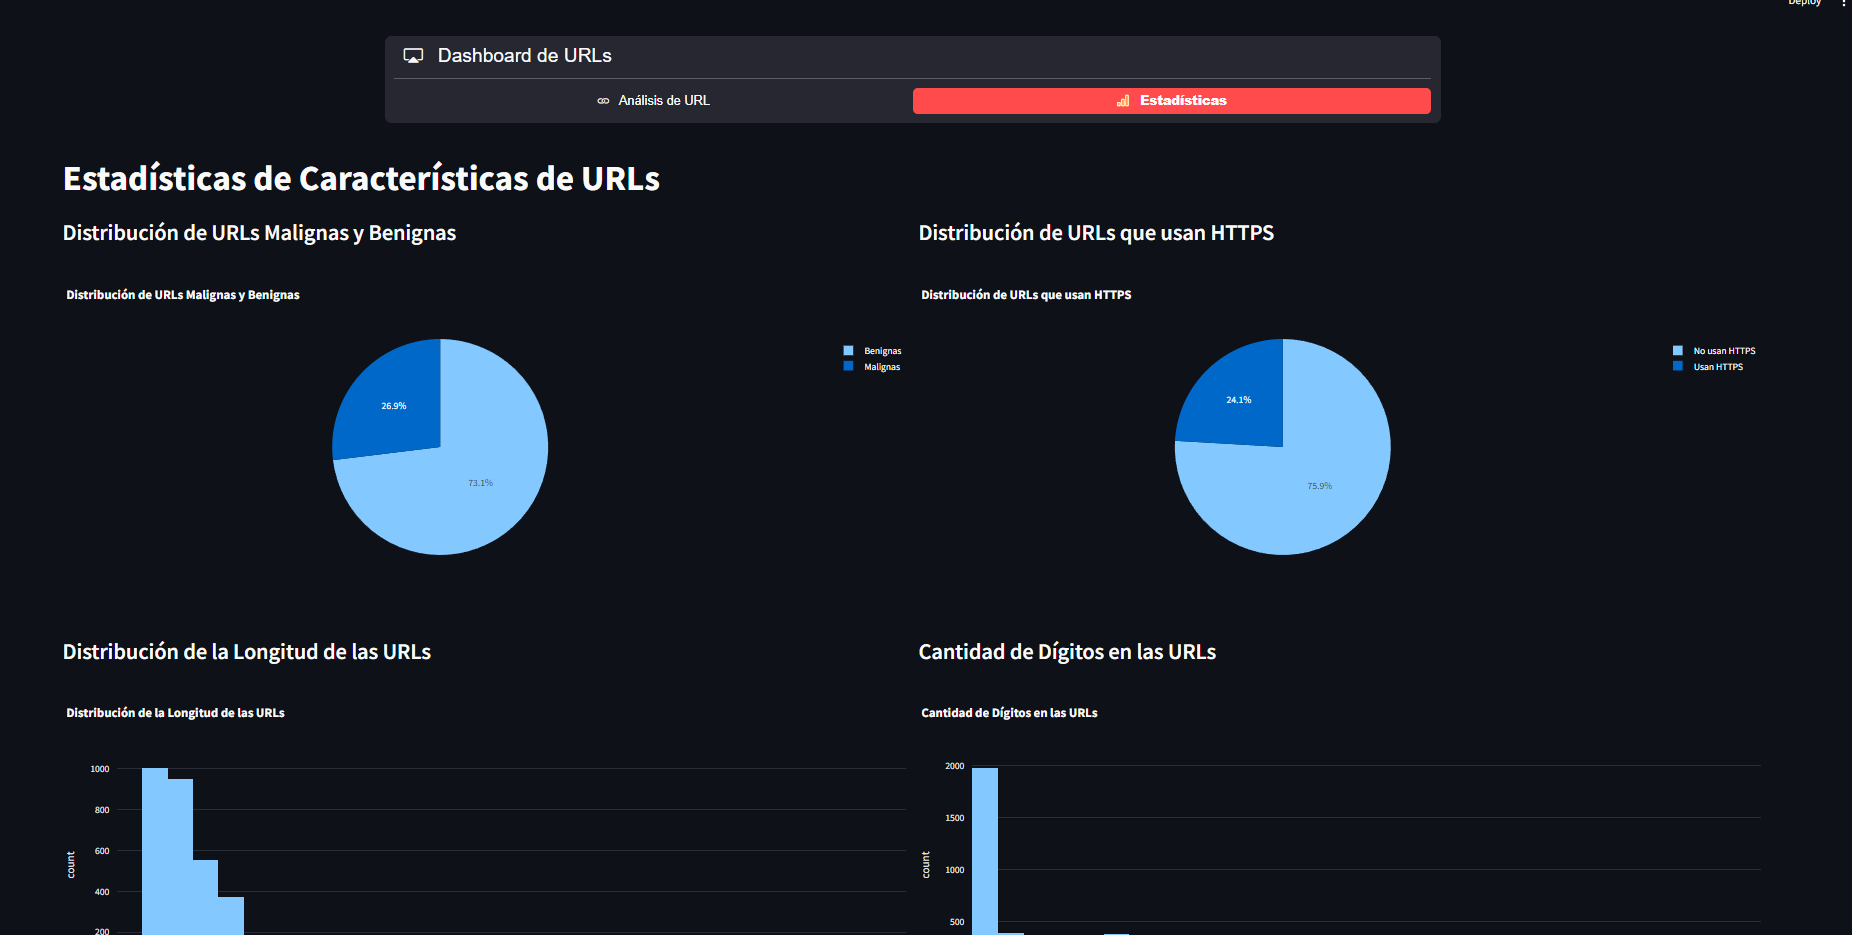
\includegraphics[width=\textwidth]{interfazEstadisticas.png}
    \caption{Vista del dashboard con estadísticas de URLs}
\end{figure}

La segunda parte del dashboard presenta una serie de gráficas que muestran estadísticas derivadas de las características de las URLs almacenadas. Estas gráficas incluyen:

\begin{itemize}
    \item Distribución de URLs Malignas y Benignas.
    \item Distribución de URLs que usan \gls{https}.
    \item Distribución de la Longitud de las URLs.
    \item Cantidad de Dígitos en las URLs.
    \item Cantidad de Letras en las URLs.
    \item Entropía del \gls{sld}.
    \item Distribución de \glspl{tld}.
    \item URLs Registradas y No Registradas.
    \item Edad de los Dominios.
    \item Mapa de Densidad de URLs Benignas y Malignas.
    \item Nube de Palabras de Palabras Sospechosas.
\end{itemize}

\subsection*{Pruebas de Evaluación}

Para evaluar la eficacia y eficiencia del dashboard, se realizaron pruebas en diferentes escenarios. A continuación, se presentan los resultados de estas pruebas:

\subsubsection*{Caso de Prueba 1: Análisis de URL Benigna}


\begin{figure}[H]
    \centering
    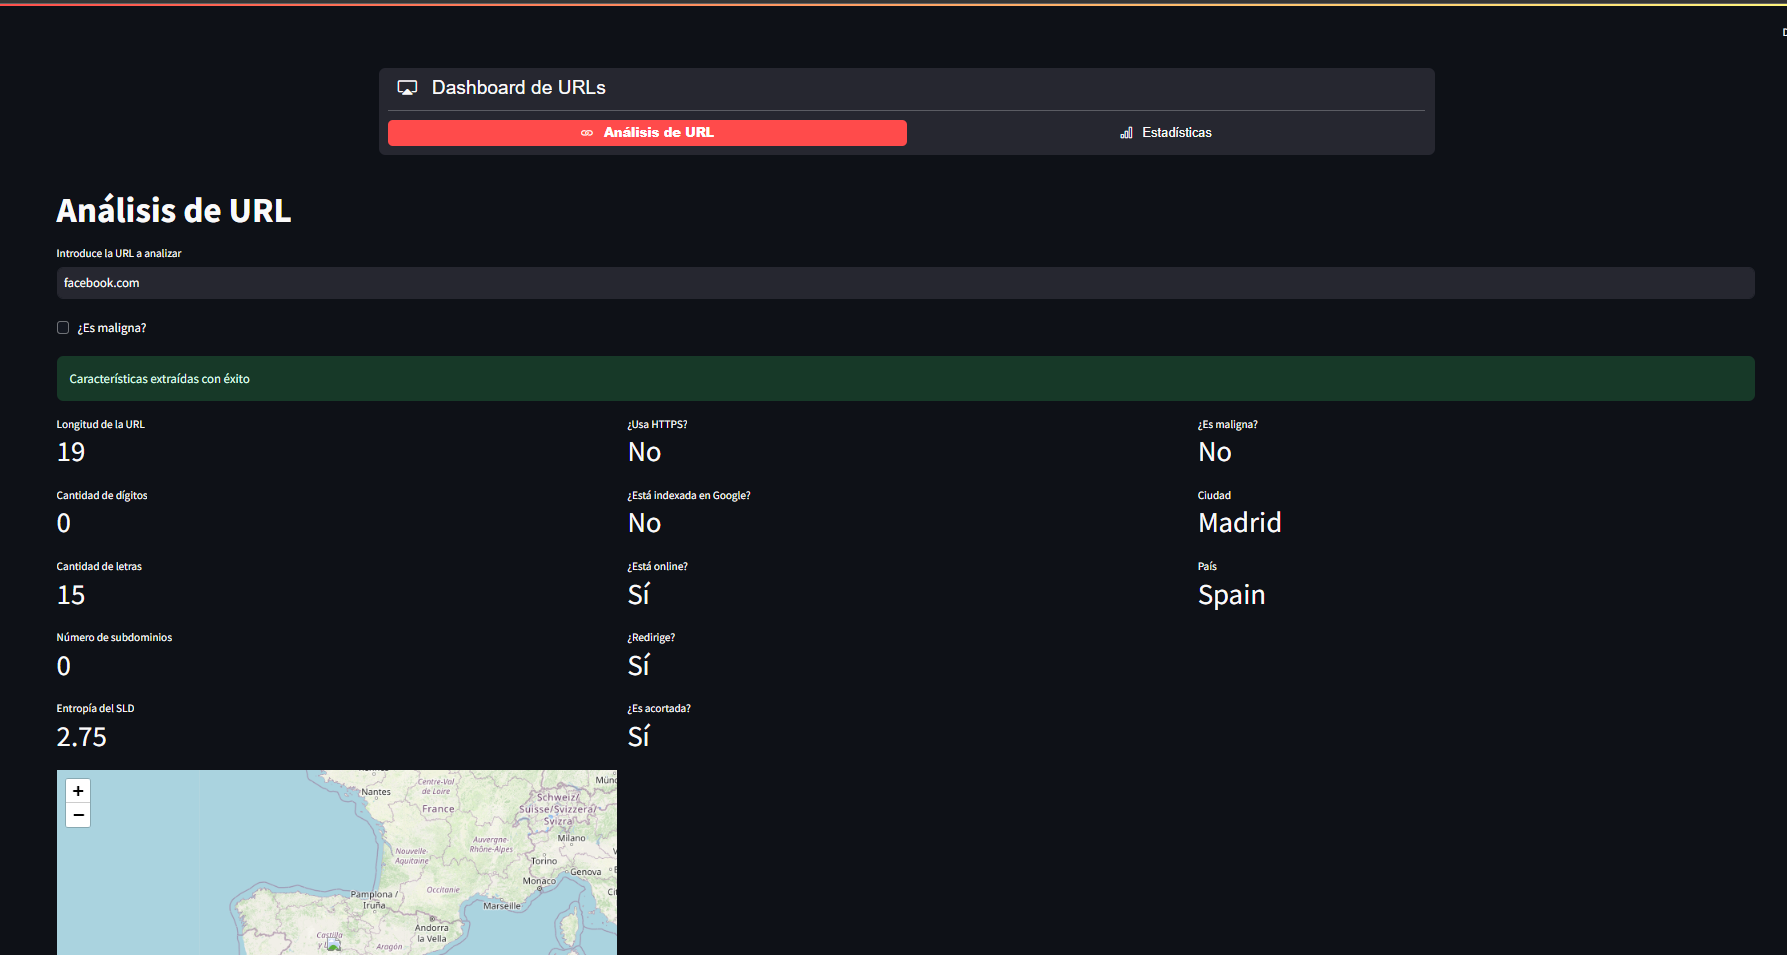
\includegraphics[width=\textwidth]{analisisUrlBenignaDashboard}
    \caption{Análisis de URL Benigna}
\end{figure}

\begin{itemize}
    \item \textbf{Descripción:} Se ingresó la URL de Facebook para el análisis.
    \item \textbf{Resultado:} El dashboard determinó correctamente que la URL es benigna, mostrando las características extraídas.
\end{itemize}



\subsection*{Interactividad y Usabilidad}

El dashboard ofrece una interfaz intuitiva y fácil de usar. Los usuarios pueden obtener información detallada sobre las URLs con solo unos pocos clics. Las gráficas interactivas permiten una exploración profunda de los datos y una mejor comprensión de las características de las URLs almacenadas.


\begin{figure}[H]
    \centering
    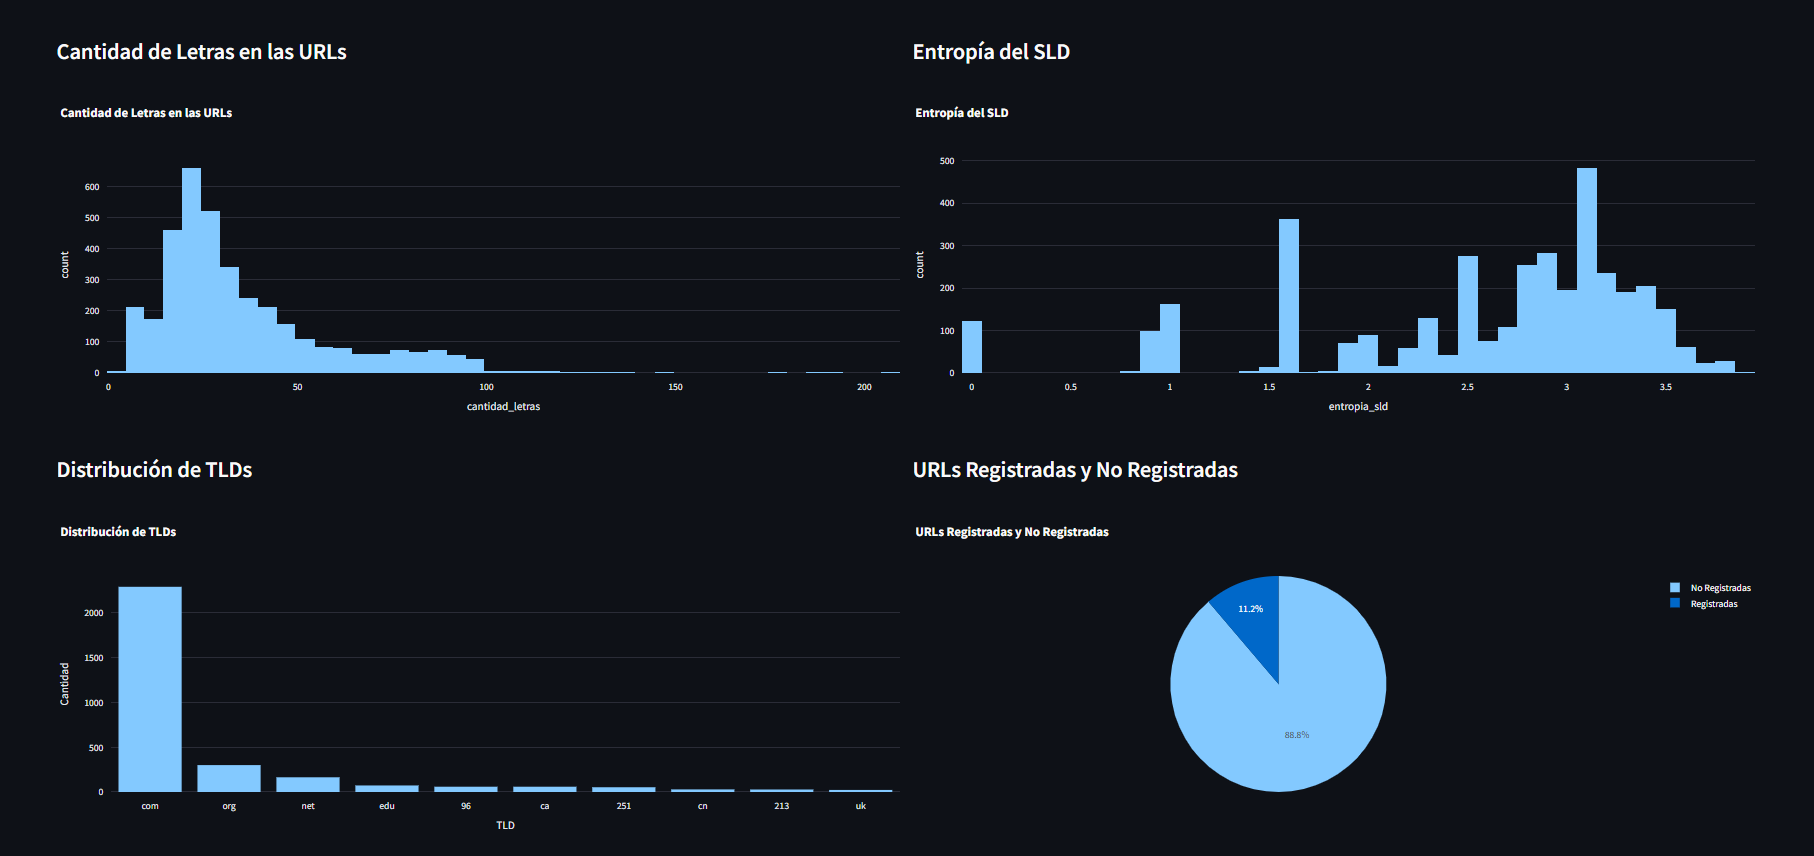
\includegraphics[width=\textwidth]{imageDashboard1.png}
    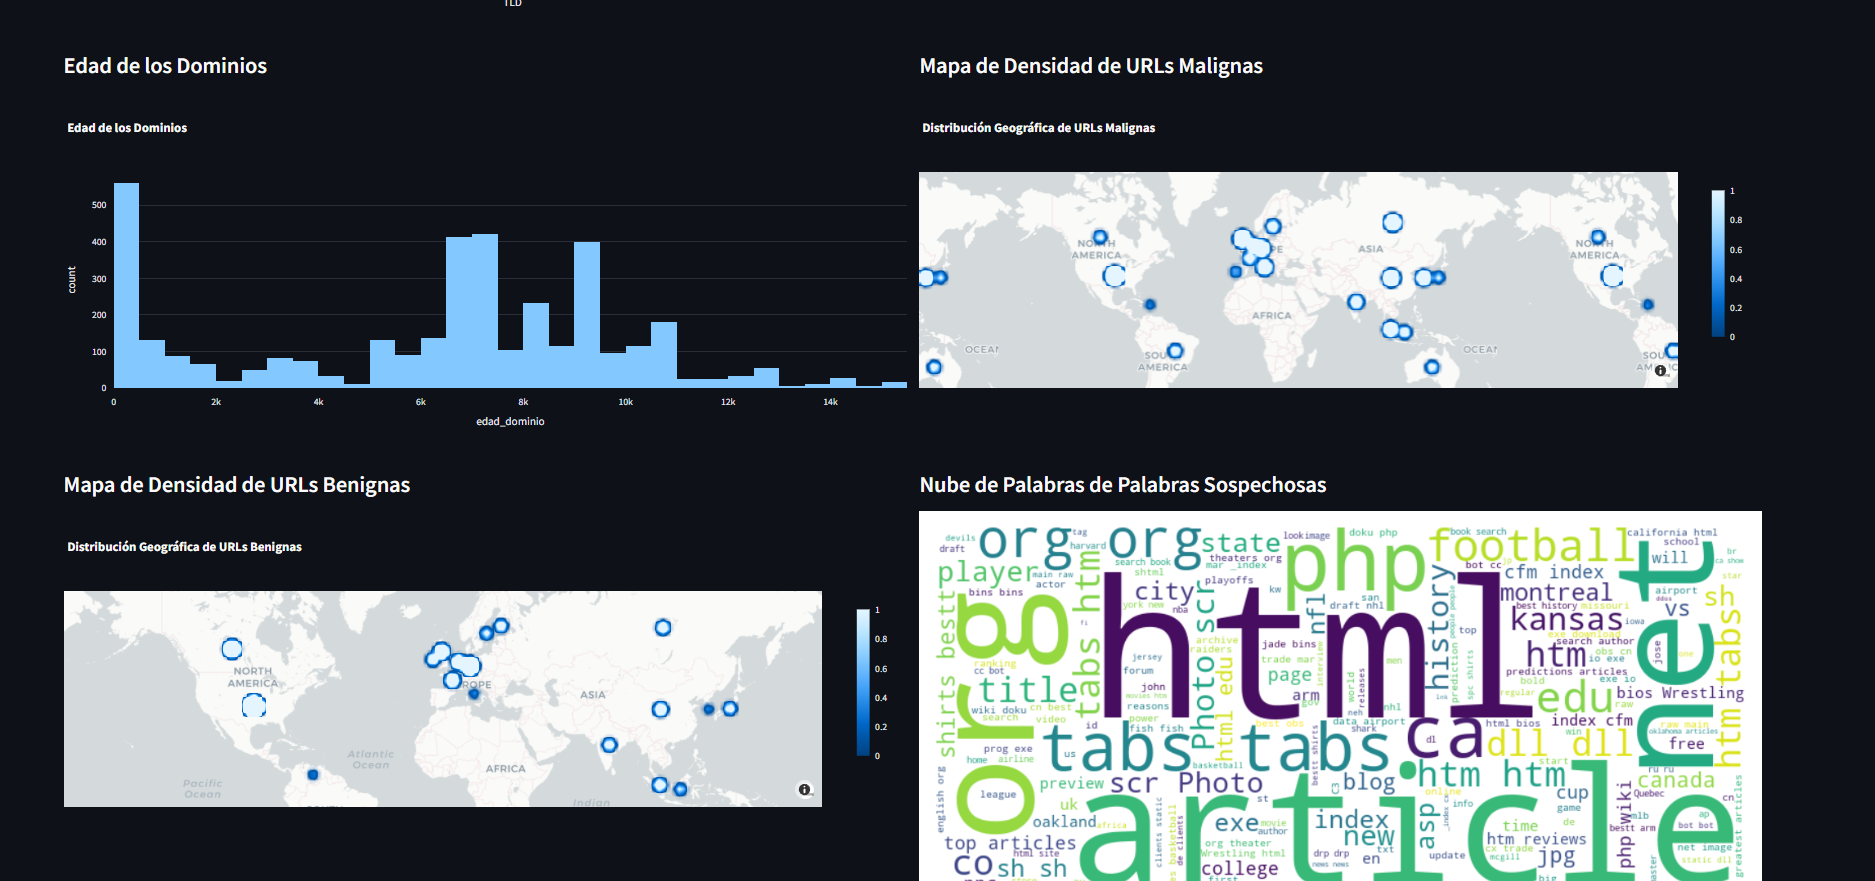
\includegraphics[width=\textwidth]{imageDashboard2.png}
    \caption{Interfaz de análisis de URL interactiva}
\end{figure}

\subsection*{Eficiencia}

El tiempo de respuesta para el análisis de una URL es de aproximadamente 5 segundos, lo cual es razonable dado el nivel de detalle del análisis realizado. Las visualizaciones en el dashboard de estadísticas son rápidas, ya que se basan en datos preextraídos.

\subsection*{Conclusión}

El \textit{Dashboard de URLs} demuestra ser una herramienta efectiva para el análisis y la visualización de características de URLs. Su capacidad para proporcionar informes detallados y visualizaciones interactivas lo convierte en una herramienta valiosa para la evaluación de la seguridad de las URLs.

\subsection*{Consideraciones Adicionales}

\begin{itemize}
    \item \textbf{Interactividad:} Las gráficas interactivas permiten a los usuarios explorar los datos de manera dinámica.
    \item \textbf{Usabilidad:} La interfaz es intuitiva y fácil de navegar.
    \item \textbf{Optimización:} Se pueden considerar mejoras en la velocidad del análisis y la incorporación de funcionalidades adicionales basadas en el feedback de los usuarios.
\end{itemize}



\newpage
\section{Conclusiones y trabajos futuros}
\subsection{Limitaciones}

El sistema de detección de URLs maliciosas desarrollado presenta varias limitaciones que deben tenerse en cuenta:

\begin{itemize}
    \item \textbf{Dependencia de la Disponibilidad de la URL:} El \textit{extractor}, que es una clase en \textit{Python}, depende de que la URL esté en línea para extraer ciertas características, como la presencia de scripts o caracteres no decodificables. Si el servidor donde está alojada la URL está muy lejos, el tiempo de extracción de características puede aumentar significativamente.
    
    \item \textbf{Rapidez del Cambio de las URLs:} Las URLs maliciosas cambian rápidamente. Los atacantes crean clones muy buenos de sitios legítimos que son difíciles de detectar. Además, las URLs maliciosas activas son difíciles de encontrar porque suelen ser eliminadas rápidamente por las autoridades o los atacantes las mantienen en línea solo por un corto periodo para evitar ser rastreadas.

    \item \textbf{Contenido Dinámico y Malicioso:} Hay sitios web que inicialmente son benignos (como \textit{GitHub}), pero que pueden alojar contenido malicioso que los usuarios pueden descargar. Asimismo, sitios como \textit{Mil Anuncios} pueden tener anuncios que son fraudulentos, aunque el sitio en sí no lo sea.

    \item \textbf{Limitaciones del Modelo:} Los modelos de \textit{machine learning} utilizados son buenos para detectar URLs maliciosas basándose en sus características, pero no analizan el contenido dentro de la página ni las acciones de los scripts presentes. Esto significa que el sistema puede no detectar actividades maliciosas que ocurren una vez que se carga la página.

    \item \textbf{Disponibilidad de Datos Maliciosos:} Es difícil obtener un conjunto de datos suficientemente amplio y representativo de URLs maliciosas activas. Muchas de estas URLs son eliminadas rápidamente, lo que dificulta su recopilación y análisis en tiempo real.
\end{itemize}

\subsection{Conclusiones}


\subsection*{Logros del Objetivo General}
El objetivo principal de este trabajo era desarrollar un sistema avanzado basado en \textit{machine learning} para la detección y clasificación de \gls{url} maliciosas, implementarlo en un entorno de tiempo real y desarrollar un \gls{dashboard} interactivo que permitiera analizar y visualizar las características y patrones comunes de las \gls{url} almacenadas en una base de datos. Este objetivo se ha cumplido satisfactoriamente, logrando un sistema eficiente y eficaz que cumple con las expectativas planteadas.

\subsection{Logros de los Objetivos Específicos}
\begin{itemize}
    \item \textbf{Desarrollar un extractor de características robusto y detallado:} Se ha implementado un extractor de características que incluye aspectos léxicos, información \gls{whois}, datos geográficos de los servidores y la presencia de patrones sospechosos en las \gls{url}. Este extractor ha demostrado ser eficiente en la recolección y análisis de datos relevantes.
    
    \item \textbf{Entrenar y evaluar un modelo de \textit{machine learning} para la detección y clasificación de \gls{url} maliciosas y benignas:} Se han entrenado y evaluado varios modelos de \textit{machine learning}, siendo el modelo de \textit{stacking} y \textit{xgboost} los más destacados. Las métricas de evaluación utilizadas fueron la precisión, el porcentaje de falsos positivos (FP) y el porcentaje de falsos negativos (FN), obteniendo resultados sobresalientes con una precisión superior al 99 por ciento.
    
    \item \textbf{Implementar el modelo entrenado en un \gls{plugin} básico para navegadores:} Se ha desarrollado un \gls{plugin} para navegadores que alerta a los usuarios cuando visitan una \gls{url} maliciosa. El \gls{plugin} ha sido probado con \glspl{url} benignas y maliciosas, demostrando su efectividad en la detección de amenazas.
    
    \item \textbf{Desarrollar un \gls{dashboard} web:} Se ha implementado un \gls{dashboard} interactivo que permite a los usuarios introducir una \gls{url} para su análisis y visualizar estadísticas y características de las \glspl{url} almacenadas en la base de datos. El \gls{dashboard} incluye gráficos y mapas interactivos que facilitan el análisis de los datos.
\end{itemize}

\subsection*{Evaluación del Modelo de Machine Learning}
Las métricas de evaluación utilizadas fueron la precisión, el porcentaje de falsos positivos (FP) y el porcentaje de falsos negativos (FN). Estas métricas fueron seleccionadas debido a su importancia en la evaluación de modelos de clasificación, especialmente en el contexto de detección de phishing y \glspl{url} maliciosas, donde es crucial minimizar tanto los falsos positivos como los falsos negativos. Los resultados obtenidos muestran que el modelo de \textit{stacking} alcanzó una precisión del 99.28, con un FP de 0.4 y un FN de 0.31 por ciento.

\subsection*{Funcionamiento del Plugin y Dashboard}
El \gls{plugin} y el \gls{dashboard} desarrollados han demostrado ser herramientas efectivas para la detección y análisis de \glspl{url} maliciosas. El \gls{plugin} funciona correctamente, alertando a los usuarios sobre posibles amenazas. El \gls{dashboard} permite un análisis detallado y visualización de las características de las \glspl{url}, proporcionando a los usuarios información valiosa de manera rápida y accesible.

\subsection*{Impacto y Contribuciones}
El trabajo realizado ha contribuido significativamente al campo de la ciberseguridad, proporcionando una herramienta avanzada para la detección de \glspl{url} maliciosas. La implementación del \gls{plugin} y \gls{dashboard} no solo mejora la seguridad de los usuarios al navegar por la web, sino que también facilita el análisis de patrones y características comunes en \glspl{url} maliciosas, lo que puede ser útil para futuras investigaciones y desarrollos en este campo.

\subsection{Trabajos Futuros}

En el futuro, se planean diversas mejoras y expansiones al sistema desarrollado para la detección de URLs maliciosas. A continuación, se detallan algunas de las direcciones de investigación y desarrollo que se consideran más prometedoras:

\begin{itemize}
    \item \textbf{Recopilación continua de URLs maliciosas:} Es esencial continuar recopilando URLs maliciosas y extrayendo sus características antes de que desaparezcan. Esto permitirá mantener actualizada la base de datos y mejorar continuamente el rendimiento de los modelos de machine learning.

    \item \textbf{Entrenamiento de mejores modelos:} Se planea entrenar modelos más avanzados que consideren una mayor cantidad de características, incluyendo tanto aspectos léxicos como características internas del diseño de la web. Esto incluye analizar qué hacen los scripts, si los textos incitan a realizar acciones fraudulentas, entre otros.

    \item \textbf{Publicación y creación de comunidad:} Se prevé publicar el plugin y el dashboard, así como crear una comunidad de usuarios que utilicen estas herramientas y enriquezcan la base de datos con nuevas URLs maliciosas. La retroalimentación y la colaboración con la comunidad serán clave para mejorar el sistema.

    \item \textbf{Modelo complementario de procesamiento de lenguaje natural:} Se propone complementar el modelo de machine learning actual con un modelo de procesamiento de lenguaje natural (NLP) para analizar el contenido de las páginas web. Esto permitirá detectar si los textos incitan a estafas u otras actividades maliciosas.

    \item \textbf{Colaboraciones con otras entidades:} Se busca establecer colaboraciones con otras entidades, como \textit{urlhaus}, para compartir información y mejorar la detección de URLs maliciosas. Estas colaboraciones pueden enriquecer la base de datos y proporcionar nuevas perspectivas y enfoques para la detección de amenazas.

    \item \textbf{Evaluación y pruebas adicionales:} Se realizarán pruebas adicionales para validar y mejorar el sistema. Esto incluirá el uso de nuevos conjuntos de datos y la evaluación en escenarios específicos para asegurar la robustez y precisión del sistema.

    \item \textbf{Publicación y difusión de resultados:} Se planea publicar los resultados de esta investigación en conferencias y revistas especializadas. Además, se buscarán formas efectivas de difundir y compartir los hallazgos con la comunidad académica y profesional.

\end{itemize}
\newpage
\section{Glosario}
%\printglossaries
\printnoidxglossaries
\newpage
%========================================================================%$$
%                                                                        %$$
%                          Bibliografia                                  %$$
%                                                                        %$$
%========================================================================%$$
                                                                         %$$
\section{Bibliografía}                                                   %$$
\printbibliography                                                       %$$
                                                                         %$$
%************************************************************************%$$
%                                                                        %$$
%                          Fin Bibliografia                              %$$
%                                                                        %$$
%========================================================================%

\newpage

%========================================================================%$$
%                                                                        %$$
%                                Anexos                                  %$$
%                                                                        %$$
%========================================================================%$$
                                                                         %$$
\section{Anexos}                                                         %$$ 
\setcounter{page}{1}                                                     %$$
\renewcommand{\thepage}{Anexo1 -\arabic{page}}                           %$$
%\subsection{Anexo: Configuración de PostgreSQL en Windows}

\subsection*{Instalación de PostgreSQL en Windows}
Para instalar PostgreSQL en Windows, se deben seguir los siguientes pasos:

\begin{enumerate}
    \item \textbf{Descarga del Instalador de PostgreSQL}:
    \begin{itemize}
        \item Visitar la página oficial de PostgreSQL: \href{https://www.postgresql.org/download/windows/}{https://www.postgresql.org/download/windows/}
        \item Descargar el instalador de la versión más reciente proporcionada por EnterpriseDB.
    \end{itemize}
    \item \textbf{Ejecución del Instalador}:
    \begin{itemize}
        \item Ejecutar el archivo de instalación descargado.
        \item Seguir las instrucciones del asistente de instalación:
        \begin{itemize}
            \item \textbf{Seleccionar directorio de instalación}: Elegir la ubicación donde se desea instalar PostgreSQL.
            \item \textbf{Seleccionar componentes}: Dejar los componentes por defecto seleccionados (PostgreSQL Server, pgAdmin 4, Stack Builder, etc.).
            \item \textbf{Configurar el superusuario}: Definir una contraseña para el usuario \texttt{postgres} (es importante recordar esta contraseña, ya que será necesaria para administrar PostgreSQL).
            \item \textbf{Seleccionar puerto}: El puerto por defecto es 5432. No es necesario cambiarlo a menos que sea estrictamente necesario.
            \item \textbf{Configuración regional}: Seleccionar la configuración regional adecuada.
        \end{itemize}
    \end{itemize}
    \item \textbf{Finalización de la Instalación}:
    \begin{itemize}
        \item Una vez completada la instalación, el asistente ofrecerá la opción de ejecutar Stack Builder. Esta opción puede desmarcarse por ahora y finalizar la instalación.
    \end{itemize}
\end{enumerate}

\subsection*{Configuración de PostgreSQL}

\subsubsection*{Acceso a la Interfaz de Línea de Comandos}
\begin{itemize}
    \item Abrir el menú de inicio y buscar \textit{SQL Shell (psql)}.
    \item Ejecutarlo y proporcionar la siguiente información cuando se solicite:
    \begin{itemize}
        \item \textbf{Server}:  [localhost]
        \item \textbf{Database}:  [postgres]
        \item \textbf{Port}:  [5432]
        \item \textbf{Username}: [postgres]
        \item \textbf{Password}
    \end{itemize}
\end{itemize}

\subsubsection*{Creación de una Base de Datos y un Usuario}
Una vez en el shell de PostgreSQL, se puede crear una nueva base de datos y un nuevo usuario con los siguientes comandos SQL:

\begin{lstlisting}[language=SQL, caption=Comandos SQL para crear una base de datos y un usuario]
CREATE DATABASE url;
CREATE USER yourusername WITH ENCRYPTED PASSWORD 'yourpassword';
GRANT ALL PRIVILEGES ON DATABASE url_classification TO yourusername;
\end{lstlisting}

\subsection*{Conexión a PostgreSQL desde Python}

\subsubsection*{Instalación de \texttt{psycopg2}}
Abrir una terminal de comandos (CMD) o PowerShell y ejecutar el siguiente comando para instalar el paquete \texttt{psycopg2}:

\begin{lstlisting}[language=bash, caption=Instalación de psycopg2]
pip install psycopg2-binary
\end{lstlisting}

\subsubsection*{Conexión a la Base de Datos desde un Script de Python}
El siguiente script de Python muestra cómo conectarse a la base de datos PostgreSQL y crear una tabla:

\begin{lstlisting}[language=Python, caption=Script de conexión a PostgreSQL y creación de tabla, breaklines=true]
import psycopg2

try:
    conn = psycopg2.connect(
        dbname="url",
        user="postgre",
        password="1234",
        host="localhost",
        port="5432"
    )
    cur = conn.cursor()
    print("Conexión exitosa a la base de datos")

    # Ejemplo de creacion de una tabla
    cur.execute("""
    CREATE TABLE IF NOT EXISTS TablaUrl (
        id SERIAL PRIMARY KEY,
        url TEXT NOT NULL,
        label BOOLEAN NOT NULL,
        domain VARCHAR(255),
        path TEXT,
        query TEXT,
        length INT,
        num_dots INT,
        num_hyphens INT,
        has_https BOOLEAN,
        has_ip BOOLEAN
    )
    """)
    conn.commit()

    # Cerrar la conexi\ón
    cur.close()
    conn.close()
    print("Tabla creada y conexion cerrada")

except Exception as e:
    print(f"Error conectando a la base de datos: {e}")
\end{lstlisting}
\newpage                                                                 %$$
%

\section*{Anexo: Procesamiento de URLs Maliciosas}

\subsection*{Descarga y Procesamiento de URLs Maliciosas}

Este script en Python descarga el archivo CSV de URLhaus, verifica si las URLs ya existen en la base de datos, y agrega las nuevas entradas.

\begin{lstlisting}[language=Python, caption=Script para procesar URLs maliciosas]
import requests
import pandas as pd
import psycopg2
from psycopg2 import sql
import io

# Configuración de la conexión a la base de datos
conn = psycopg2.connect(
    dbname="url",
    user="postgres",
    password="1234",
    host="localhost",
    port="5432"
)
cur = conn.cursor()

# Descargar el archivo CSV
csv_url = 'https://urlhaus.abuse.ch/downloads/csv_recent/'
response = requests.get(csv_url)
csv_data = response.content.decode('utf-8')

# Procesar el contenido para obtener la cabecera correcta
csv_lines = csv_data.splitlines()
header_index = next(i for i, line in enumerate(csv_lines) if line.startswith('# id'))
header = csv_lines[header_index].lstrip('# ').split(',')
csv_data = '\n'.join(csv_lines[header_index+1:])

# Leer el CSV en un DataFrame
df = pd.read_csv(io.StringIO(csv_data), names=header)

# Mostrar las primeras filas del DataFrame para verificar
print("Columnas del DataFrame:", df.columns)
print("Primeras filas del DataFrame:\n", df.head())

# Asegurarse de que las columnas estén en minúsculas
df.columns = [col.lower() for col in df.columns]

# Crear la tabla si no existe
cur.execute("""
CREATE TABLE IF NOT EXISTS TablaURL (
    url TEXT PRIMARY KEY,
    maligna BOOLEAN NOT NULL,
    tipo TEXT NOT NULL
)
""")
conn.commit()

# Procesar y agregar las URLs a la base de datos
for _, row in df.iterrows():
    url = row['url']
    threat = row['threat'] if pd.notnull(row['threat']) else '1'

    # Comprobar si la URL ya está en la base de datos
    cur.execute("SELECT EXISTS(SELECT 1 FROM TablaURL WHERE url=%s)", (url,))
    exists = cur.fetchone()[0]

    if not exists:
        # Insertar la URL en la base de datos
        cur.execute(
            sql.SQL("INSERT INTO TablaURL (url, maligna, tipo) VALUES (%s, %s, %s)"),
            (url, True, threat)
        )

conn.commit()

# Cerrar la conexión
cur.close()
conn.close()

print("Proceso completado.")
\end{lstlisting}

\subsection*{Explicación del Código}

\begin{itemize}
    \item \textbf{Configuración de la Conexión}: Se configura la conexión a la base de datos PostgreSQL con las credenciales y parámetros correspondientes.
    \item \textbf{Descarga del Archivo CSV}: Se utiliza \texttt{requests} para descargar el archivo CSV desde la URL proporcionada.
    \item \textbf{Procesamiento del CSV}: Se procesa el contenido del CSV para obtener la cabecera correcta, omitiendo los comentarios.
    \item \textbf{Lectura del CSV}: Se lee el contenido del CSV en un DataFrame de \texttt{pandas}.
    \item \textbf{Verificación de Datos}: Se imprimen las columnas y las primeras filas del DataFrame para verificar que los datos se han cargado correctamente.
    \item \textbf{Creación de la Tabla}: Si la tabla \texttt{TablaURL} no existe, se crea con las columnas \texttt{url}, \texttt{maligna} y \texttt{tipo}.
    \item \textbf{Procesamiento de Datos}: Se itera sobre las filas del DataFrame, verificando si cada URL ya está en la base de datos. Si la URL no está en la base de datos, se inserta con los valores correspondientes (\texttt{maligna=True} y \texttt{tipo} según el \texttt{threat} del CSV).
    \item \textbf{Cierre de la Conexión}: Se cierra la conexión a la base de datos.
\end{itemize}



\subsection*{Procesamiento y Almacenamiento de URLs desde Archivos JSON}

Este script en Python procesa archivos JSON grandes con URLs benignas y de phishing, y almacena las URLs en una base de datos PostgreSQL.

\begin{lstlisting}[language=Python, caption=Script para procesar archivos JSON grandes y poblar la base de datos]
import pandas as pd
import psycopg2
from psycopg2 import sql
import requests
import io

# Configuración de la conexión a la base de datos
conn = psycopg2.connect(
    dbname="url",
    user="postgres",
    password="1234",
    host="localhost",
    port="5432"
)
cur = conn.cursor()

# URLs de los archivos JSON
benign_url = 'https://zenodo.org/records/8364668/files/benign_2307.json'
phishing_url = 'https://zenodo.org/records/8364668/files/phishing_2307.json'

# Función para leer y procesar JSON en streaming
def read_and_process_json(url, maligna_value):
    response = requests.get(url, stream=True)
    response.raise_for_status()

    for chunk in response.iter_content(chunk_size=1024*1024):
        if chunk:
            data = io.StringIO(chunk.decode('utf-8'))
            df = pd.read_json(data, lines=True)
            for index, row in df.iterrows():
                domain_name = row['domain_name']
                maligna = maligna_value
                tipo = 'benign' if maligna_value == 0 else 'malicious'
                
                # Comprobar si la URL ya está en la base de datos
                cur.execute("SELECT EXISTS(SELECT 1 FROM TablaURL WHERE url=%s)", (domain_name,))
                exists = cur.fetchone()[0]

                if not exists:
                    # Insertar la URL en la base de datos
                    cur.execute(
                        sql.SQL("INSERT INTO TablaURL (url, maligna, tipo) VALUES (%s, %s, %s)"),
                        (domain_name, maligna, tipo)
                    )

    conn.commit()

# Leer y procesar los archivos JSON
read_and_process_json(benign_url, 0)
read_and_process_json(phishing_url, 1)

# Cerrar la conexión
cur.close()
conn.close()

print("Proceso completado.")
\end{lstlisting}

\section*{Explicación del Código}

\begin{itemize}
    \item \textbf{Configuración de la Conexión}: Se configura la conexión a la base de datos PostgreSQL con las credenciales y parámetros correspondientes.
    \item \textbf{URLs de los Archivos JSON}: Se definen las URLs de los archivos JSON de benignos y phishing.
    \item \textbf{Función para Leer y Procesar JSON en Streaming}: La función \texttt{read\_and\_process\_json} descarga y procesa los archivos JSON en streaming para manejar archivos grandes sin cargar todo el contenido en memoria.
    \item \textbf{Procesamiento de Datos}: Cada dominio se verifica en la base de datos para evitar duplicados. Los dominios se insertan en la tabla \texttt{TablaURL} con sus etiquetas correspondientes (\texttt{maligna} y \texttt{tipo}).
    \item \textbf{Lectura y Procesamiento de Archivos JSON}: Se procesan y agregan los datos de benignos y phishing a la base de datos.
    \item \textbf{Cierre de la Conexión}: Se cierra la conexión a la base de datos.
\end{itemize}
                                                 %$$
\newpage 
%\subsection{Anexo: Poblar Tabla Dominios de Kaggle}

\subsection*{Descarga y Procesamiento de Dominios de Kaggle}

Este script en Python descarga un dataset de dominios desde Kaggle, verifica si los dominios ya existen en la base de datos, y agrega las nuevas entradas.

\begin{lstlisting}[language=Python, caption=Script para procesar dominios de Kaggle]
import os
import kaggle
import pandas as pd
import psycopg2
from psycopg2 import sql
import zipfile

# Configuración de la conexión a la base de datos
conn = psycopg2.connect(
    dbname="url",
    user="postgres",
    password="1234",
    host="localhost",
    port="5432"
)
cur = conn.cursor()

# Configurar la API de Kaggle
os.environ['KAGGLE_CONFIG_DIR'] = os.getcwd()

# Descargar el dataset de Kaggle
dataset_path = './'
kaggle.api.dataset_download_files(
    'aayushah19/dga-or-benign-domain-names', path=dataset_path, unzip=False)

# Buscar el archivo ZIP descargado
zip_file = None
for file in os.listdir(dataset_path):
    if file.endswith('.zip'):
        zip_file = os.path.join(dataset_path, file)
        break

if not zip_file:
    raise FileNotFoundError("El archivo ZIP no se encuentra en el directorio especificado.")

# Descomprimir el archivo ZIP
with zipfile.ZipFile(zip_file, 'r') as zip_ref:
    zip_ref.extractall(dataset_path)

# Buscar el archivo CSV descomprimido
csv_file = None
for file in os.listdir(dataset_path):
    if file.endswith('.csv'):
        csv_file = os.path.join(dataset_path, file)
        break

if not csv_file:
    raise FileNotFoundError("El archivo CSV no se encuentra después de descomprimir el ZIP.")

# Leer el CSV en un DataFrame
df = pd.read_csv(csv_file)

# Limpiar los datos
df['domain'] = df['domain'].astype(str).str.strip()
df = df.dropna(subset=['domain'])

# Crear la tabla si no existe
cur.execute("""
CREATE TABLE IF NOT EXISTS dominios (
    domain TEXT PRIMARY KEY,
    benigno BOOLEAN NOT NULL
)
""")
conn.commit()

# Procesar y agregar los dominios a la base de datos
for _, row in df.iterrows():
    domain = row['domain']
    benigno = row['label'] == 'benign'

    # Comprobar si el dominio ya está en la base de datos
    cur.execute("SELECT EXISTS(SELECT 1 FROM dominios WHERE domain=%s)", (domain,))
    exists = cur.fetchone()[0]

    if not exists:
        # Insertar el dominio en la base de datos
        cur.execute(
            sql.SQL("INSERT INTO dominios (domain, benigno) VALUES (%s, %s)"),
            (domain, benigno)
        )

conn.commit()

# Cerrar la conexión
cur.close()
conn.close()

print("Proceso completado.")
\end{lstlisting}

\subsection*{Explicación del Código}

\begin{itemize}
    \item \textbf{Configuración de la Conexión}: Se configura la conexión a la base de datos PostgreSQL con las credenciales y parámetros correspondientes.
    \item \textbf{Configuración de la API de Kaggle}: Se establece la ruta del archivo \texttt{kaggle.json} que contiene las credenciales de la API.
    \item \textbf{Descarga del Dataset de Kaggle}: Se utiliza la API de Kaggle para descargar el archivo ZIP del dataset.
    \item \textbf{Descompresión del ZIP}: Se descomprime el archivo ZIP descargado para acceder al archivo CSV.
    \item \textbf{Lectura del CSV}: Se lee el archivo CSV en un DataFrame de \texttt{pandas}.
    \item \textbf{Limpieza de Datos}: Se limpian los datos del DataFrame, eliminando espacios en blanco y filas con valores nulos en la columna \texttt{domain}.
    \item \textbf{Creación de la Tabla \texttt{dominios}}: Si la tabla \texttt{dominios} no existe, se crea con las columnas \texttt{domain} y \texttt{benigno}.
    \item \textbf{Procesamiento de Datos}: Se itera sobre las filas del DataFrame, verificando si cada dominio ya está en la base de datos. Si el dominio no está en la base de datos, se inserta con los valores correspondientes (\texttt{benigno=True} o \texttt{benigno=False}).
    \item \textbf{Cierre de la Conexión}: Se cierra la conexión a la base de datos.
\end{itemize}%$$
%\subsection{Anexo: Tabla Queries}

\subsection*{Descarga y Procesamiento de Queries desde GitHub}

Este script en Python descarga archivos de texto con buenas y malas queries, verifica si las queries ya existen en la base de datos, y agrega las nuevas entradas.

\begin{lstlisting}[language=Python, caption=Script para procesar queries desde archivos de texto]
import requests
import psycopg2
from psycopg2 import sql

# Configuración de la conexión a la base de datos
conn = psycopg2.connect(
    dbname="url",
    user="postgres",
    password="1234",
    host="localhost",
    port="5432"
)
cur = conn.cursor()

# URLs de los archivos de queries en GitHub
good_queries_url = 'https://raw.githubusercontent.com/faizann24/Fwaf-Machine-Learning-driven-Web-Application-Firewall/master/goodqueries.txt'
bad_queries_url = 'https://raw.githubusercontent.com/faizann24/Fwaf-Machine-Learning-driven-Web-Application-Firewall/master/badqueries.txt'

# Función para descargar y leer archivos de texto
def download_and_read_text(url):
    response = requests.get(url)
    response.raise_for_status()
    return response.text.splitlines()

# Descargar y leer los archivos de queries
good_queries = download_and_read_text(good_queries_url)
bad_queries = download_and_read_text(bad_queries_url)

# Crear la tabla de queries si no existe
cur.execute("""
CREATE TABLE IF NOT EXISTS Queries (
    id SERIAL PRIMARY KEY,
    query TEXT NOT NULL,
    buena BOOLEAN NOT NULL
)
""")
conn.commit()

# Función para procesar y agregar queries a la base de datos
def process_and_insert_queries(queries, buena):
    for query in queries:
        # Comprobar si la query ya está en la base de datos
        cur.execute("SELECT EXISTS(SELECT 1 FROM Queries WHERE query=%s)", (query,))
        exists = cur.fetchone()[0]

        if not exists:
            # Insertar la query en la base de datos
            cur.execute(
                sql.SQL("INSERT INTO Queries (query, buena) VALUES (%s, %s)"),
                (query, buena)
            )
    conn.commit()

# Procesar y agregar las good queries
process_and_insert_queries(good_queries, True)

# Procesar y agregar las bad queries
process_and_insert_queries(bad_queries, False)

# Cerrar la conexión
cur.close()
conn.close()

print("Proceso completado.")
\end{lstlisting}

\subsection*{Explicación del Código}

\begin{itemize}
    \item \textbf{Configuración de la Conexión}: Se configura la conexión a la base de datos PostgreSQL con las credenciales y parámetros correspondientes.
    \item \textbf{URLs de los Archivos de Queries en GitHub}: Se definen las URLs de los archivos de queries de buenas y malas en GitHub.
    \item \textbf{Función para Descargar y Leer Archivos de Texto}: Se define una función para descargar y leer los archivos de texto desde las URLs proporcionadas.
    \item \textbf{Descarga y Lectura de los Archivos de Queries}: Se descargan y leen los archivos de queries.
    \item \textbf{Creación de la Tabla de Queries}: Se crea la tabla \texttt{Queries} con columnas \texttt{id}, \texttt{query} y \texttt{buena} si no existe.
    \item \textbf{Función para Procesar y Agregar Queries a la Base de Datos}: Se define una función para procesar los datos y agregarlos a la base de datos.
    \item \textbf{Verificación y Adición de Queries}: Se verifica si la query ya existe en la base de datos para evitar duplicados y se insertan las queries en la base de datos con las etiquetas correspondientes (\texttt{buena=True} o \texttt{buena=False}).
    \item \textbf{Procesamiento de Good Queries y Bad Queries}: Se procesan y agregan las good queries y bad queries a la base de datos.
    \item \textbf{Cierre de la Conexión}: Se cierra la conexión a la base de datos.
\end{itemize}




\chapter*{Anexo: Creación de Tabla con Palabras Sospechosas y Comunes}

\section*{Descarga y Almacenamiento de Palabras}

Este script en Python descarga listas de palabras sospechosas y comunes, y las almacena en una tabla de la base de datos PostgreSQL para su posterior análisis.

\begin{lstlisting}[language=Python, caption=Script para crear y poblar la tabla de palabras sospechosas y comunes]
import psycopg2
from psycopg2 import sql
import requests

# Configuración de la conexión a la base de datos
conn = psycopg2.connect(
    dbname="url",
    user="postgres",
    password="1234",
    host="localhost",
    port="5432"
)
cur = conn.cursor()

# URLs de las listas de palabras
suspicious_words_url = 'https://raw.githubusercontent.com/danielmiessler/SecLists/master/Discovery/Web-Content/raft-large-words.txt'
common_passwords_url = 'https://raw.githubusercontent.com/danielmiessler/SecLists/master/Passwords/Common-Credentials/10k-most-common.txt'

# Función para descargar y leer archivos de texto
def download_and_read_text(url):
    response = requests.get(url)
    response.raise_for_status()
    return response.text.splitlines()

# Descargar y leer las listas de palabras
suspicious_words = download_and_read_text(suspicious_words_url)
common_passwords = download_and_read_text(common_passwords_url)

# Crear la tabla de palabras si no existe
cur.execute("""
CREATE TABLE IF NOT EXISTS Palabras (
    id SERIAL PRIMARY KEY,
    palabra TEXT NOT NULL,
    tipo TEXT NOT NULL
)
""")
conn.commit()

# Función para insertar palabras en la base de datos
def insert_words(words, tipo):
    data_to_insert = [(word, tipo) for word in words]
    cur.executemany(
        sql.SQL("INSERT INTO Palabras (palabra, tipo) VALUES (%s, %s) ON CONFLICT DO NOTHING"),
        data_to_insert
    )
    conn.commit()

# Insertar las palabras sospechosas y comunes en la base de datos
insert_words(suspicious_words, 'suspicious')
insert_words(common_passwords, 'common_password')

# Cerrar la conexión
cur.close()
conn.close()

print("Proceso completado.")
\end{lstlisting}

\section*{Explicación del Código}

\begin{itemize}
    \item \textbf{Configuración de la Conexión}: Se configura la conexión a la base de datos PostgreSQL con las credenciales y parámetros correspondientes.
    \item \textbf{URLs de las Listas de Palabras}: Se definen las URLs de las listas de palabras sospechosas y comunes.
    \item \textbf{Función para Descargar y Leer Archivos de Texto}: La función \texttt{download\_and\_read\_text} descarga y lee los archivos de texto desde las URLs proporcionadas.
    \item \textbf{Descarga y Lectura de las Listas de Palabras}: Se descargan y leen las listas de palabras sospechosas y comunes.
    \item \textbf{Creación de la Tabla de Palabras}: Se crea la tabla \texttt{Palabras} con columnas \texttt{id}, \texttt{palabra} y \texttt{tipo} si no existe.
    \item \textbf{Función para Insertar Palabras en la Base de Datos}: La función \texttt{insert\_words} inserta las palabras en la base de datos, etiquetándolas como \texttt{suspicious} o \texttt{common\_password}.
    \item \textbf{Inserción de Palabras}: Se insertan las palabras sospechosas y comunes en la base de datos.
    \item \textbf{Cierre de la Conexión}: Se cierra la conexión a la base de datos.
\end{itemize}


\chapter*{Anexo: Creación y Población de Tablas WHOIS y Geolocalización}

\section*{Creación de Tablas}

Este script en Python crea las tablas \texttt{WHOIS} y \texttt{Geolocalizacion} para almacenar información WHOIS y de geolocalización para los dominios asociados con las URLs.

\begin{lstlisting}[language=Python, caption=Creación de las tablas WHOIS y Geolocalizacion]
import psycopg2

# Configuración de la conexión a la base de datos
conn = psycopg2.connect(
    dbname="url",
    user="postgres",
    password="1234",
    host="localhost",
    port="5432"
)
cur = conn.cursor()

# Crear la tabla WHOIS si no existe
cur.execute("""
CREATE TABLE IF NOT EXISTS WHOIS (
    id SERIAL PRIMARY KEY,
    domain TEXT NOT NULL,
    creation_date DATE,
    expiration_date DATE,
    registrant_name TEXT,
    registrant_organization TEXT,
    registrant_country TEXT,
    FOREIGN KEY (domain) REFERENCES TablaURL (url)
)
""")
conn.commit()

# Crear la tabla Geolocalizacion si no existe
cur.execute("""
CREATE TABLE IF NOT EXISTS Geolocalizacion (
    id SERIAL PRIMARY KEY,
    ip TEXT NOT NULL,
    country TEXT,
    region TEXT,
    city TEXT,
    latitude DOUBLE PRECISION,
    longitude DOUBLE PRECISION,
    FOREIGN KEY (ip) REFERENCES TablaURL (url)
)
""")
conn.commit()

# Cerrar la conexión
cur.close()
conn.close()

print("Tablas WHOIS y Geolocalizacion creadas exitosamente.")
\end{lstlisting}



\section*{Explicación del Código}

\begin{itemize}
    \item \textbf{Configuración de la Conexión}: Se configura la conexión a la base de datos PostgreSQL con las credenciales y parámetros correspondientes.
    \item \textbf{Creación de la Tabla WHOIS}: La tabla \texttt{WHOIS} almacena información WHOIS para dominios asociados con las URLs.
    \item \textbf{Creación de la Tabla Geolocalizacion}: La tabla \texttt{Geolocalizacion} almacena datos de geolocalización para las IPs asociadas con las URLs.
    \item \textbf{Cierre de la Conexión}: Se cierra la conexión a la base de datos.
\end{itemize}


\chapter*{Anexo: Creación y Población de la Tabla de TLDs}

\section*{Creación de la Tabla TLDs}

Este script en Python crea una tabla \texttt{TLDs} para almacenar información sobre los Top-Level Domains (TLDs) y sus características.

\begin{lstlisting}[language=Python, caption=Creación de la tabla TLDs con restricción única]
import requests
import psycopg2
from psycopg2 import sql
from bs4 import BeautifulSoup

# Configuración de la conexión a la base de datos
conn = psycopg2.connect(
    dbname="url",
    user="postgres",
    password="1234",
    host="localhost",
    port="5432"
)
cur = conn.cursor()

# Crear la tabla TLDs si no existe con una restricción única en la columna DOMAIN
cur.execute("""
CREATE TABLE IF NOT EXISTS TLDs (
    id SERIAL PRIMARY KEY,
    domain TEXT NOT NULL UNIQUE,
    type TEXT,
    tld_manager TEXT
)
""")
conn.commit()

# Función para obtener TLDs de IANA
def get_tlds_from_iana():
    url = 'https://www.iana.org/domains/root/db'
    response = requests.get(url)
    response.raise_for_status()
    soup = BeautifulSoup(response.text, 'html.parser')
    tld_list = []

    for row in soup.select('table tbody tr'):
        columns = row.find_all('td')
        if len(columns) >= 3:
            domain = columns[0].text.strip()
            tld_type = columns[1].text.strip()
            tld_manager = columns[2].text.strip()
            tld_list.append((domain, tld_type, tld_manager))

    return tld_list

# Obtener TLDs y sus características
tlds = get_tlds_from_iana()

# Insertar TLDs en la base de datos
cur.executemany(
    sql.SQL("INSERT INTO TLDs (domain, type, tld_manager) VALUES (%s, %s, %s) ON CONFLICT (domain) DO NOTHING"),
    tlds
)
conn.commit()

# Cerrar la conexión
cur.close()
conn.close()

print("Tabla TLDs creada y poblada exitosamente.")
\end{lstlisting}

\section*{Explicación del Código}

\begin{itemize}
    \item \textbf{Configuración de la Conexión}: Se configura la conexión a la base de datos PostgreSQL con las credenciales y parámetros correspondientes.
    \item \textbf{Creación de la Tabla TLDs con Restricción Única}: La tabla \texttt{TLDs} almacena información sobre los TLDs y sus características, y la columna \texttt{domain} se define como \texttt{UNIQUE}.
    \item \textbf{Función para Obtener TLDs de IANA}: La función \texttt{get\_tlds\_from\_iana} descarga y analiza la lista de TLDs de IANA.
    \item \textbf{Inserción de TLDs en la Base de Datos}: Se insertan los TLDs y sus características en la tabla \texttt{TLDs}. La cláusula \texttt{ON CONFLICT (domain) DO NOTHING} asegura que los dominios duplicados no se inserten.
    \item \textbf{Cierre de la Conexión}: Se cierra la conexión a la base de datos.
\end{itemize}


.
\renewcommand{\thepage}{Anexo 2 -\arabic{page}}
                                                                         %$$
%************************************************************************%$$
%                                                                        %$$
%                               Anexos                                   %$$
%                                                                        %$$
%========================================================================%$$





%\lipsum[1-3]
% ... el resto de tu documento ...

\end{document}